\documentclass[12pt,]{book}
\usepackage{lmodern}
\usepackage{amssymb,amsmath}
\usepackage{ifxetex,ifluatex}
\usepackage{fixltx2e} % provides \textsubscript
\ifnum 0\ifxetex 1\fi\ifluatex 1\fi=0 % if pdftex
  \usepackage[T1]{fontenc}
  \usepackage[utf8]{inputenc}
\else % if luatex or xelatex
  \ifxetex
    \usepackage{mathspec}
  \else
    \usepackage{fontspec}
  \fi
  \defaultfontfeatures{Ligatures=TeX,Scale=MatchLowercase}
\fi
% use upquote if available, for straight quotes in verbatim environments
\IfFileExists{upquote.sty}{\usepackage{upquote}}{}
% use microtype if available
\IfFileExists{microtype.sty}{%
\usepackage{microtype}
\UseMicrotypeSet[protrusion]{basicmath} % disable protrusion for tt fonts
}{}
\usepackage[margin=1in]{geometry}
\usepackage{hyperref}
\hypersetup{unicode=true,
            pdftitle={Challenges and Tools in the Assessment and Management of Pacific Salmon Fisheries},
            pdfauthor={Ben Staton},
            pdfborder={0 0 0},
            breaklinks=true}
\urlstyle{same}  % don't use monospace font for urls
\usepackage{natbib}
\bibliographystyle{myapalike}
\usepackage{longtable,booktabs}
\usepackage{graphicx,grffile}
\makeatletter
\def\maxwidth{\ifdim\Gin@nat@width>\linewidth\linewidth\else\Gin@nat@width\fi}
\def\maxheight{\ifdim\Gin@nat@height>\textheight\textheight\else\Gin@nat@height\fi}
\makeatother
% Scale images if necessary, so that they will not overflow the page
% margins by default, and it is still possible to overwrite the defaults
% using explicit options in \includegraphics[width, height, ...]{}
\setkeys{Gin}{width=\maxwidth,height=\maxheight,keepaspectratio}
\IfFileExists{parskip.sty}{%
\usepackage{parskip}
}{% else
\setlength{\parindent}{0pt}
\setlength{\parskip}{6pt plus 2pt minus 1pt}
}
\setlength{\emergencystretch}{3em}  % prevent overfull lines
\providecommand{\tightlist}{%
  \setlength{\itemsep}{0pt}\setlength{\parskip}{0pt}}
\setcounter{secnumdepth}{5}
% Redefines (sub)paragraphs to behave more like sections
\ifx\paragraph\undefined\else
\let\oldparagraph\paragraph
\renewcommand{\paragraph}[1]{\oldparagraph{#1}\mbox{}}
\fi
\ifx\subparagraph\undefined\else
\let\oldsubparagraph\subparagraph
\renewcommand{\subparagraph}[1]{\oldsubparagraph{#1}\mbox{}}
\fi

%%% Use protect on footnotes to avoid problems with footnotes in titles
\let\rmarkdownfootnote\footnote%
\def\footnote{\protect\rmarkdownfootnote}

%%% Change title format to be more compact
\usepackage{titling}

% Create subtitle command for use in maketitle
\newcommand{\subtitle}[1]{
  \posttitle{
    \begin{center}\large#1\end{center}
    }
}

\setlength{\droptitle}{-2em}

  \title{Challenges and Tools in the Assessment and Management of Pacific Salmon
Fisheries}
    \pretitle{\vspace{\droptitle}\centering\huge}
  \posttitle{\par}
    \author{Ben Staton}
    \preauthor{\centering\large\emph}
  \postauthor{\par}
    \date{}
    \predate{}\postdate{}
  
\usepackage{booktabs}
%%% This is an example file for the Auburn University style options
%%%       aums.sty (Masters Thesis)
%%%       auphd.sty (Ph.D. Dissertation)
%%%       auhonors.sty (Honors Scholar)

%%%To use it, please edit the necessary options, title, author, date, year, keywords, advisor, professor, etc. 

% \documentclass[12pt]{report}
\usepackage{setspace}
% \usepackage{titlesec}
%\setcounter{secnumdepth}{3}
% \usepackage{aums}       % For Master's papers
\usepackage{auphd}     % For Ph.D.
%\usepackage{auhonors}  % For honors college
\usepackage[normalem]{ulem}       % underlining on style-page; see \normalem below
\usepackage{url}
\usepackage[table]{xcolor}
\usepackage{tikz}
\usepackage{pgf}
\usepackage{color,soul}
\usepackage{float}
\usepackage{caption}
\captionsetup{width=\textwidth}

\usepackage{amsmath,amsthm, amsfonts, mathrsfs, graphicx, setspace, fullpage, color}
\usepackage{natbib, appendix}
\usepackage[T1]{fontenc}
\usepackage{multirow}
\usepackage{mathabx}
\RequirePackage{adjustbox}
% \usepackage{epstopdf}
\AtBeginDocument{\renewcommand{\bibname}{References}}
\usepackage{hyperref}
\usepackage[hang,flushmargin]{footmisc}
%\usepackage{tocloft}
%\renewcommand\cftchapafterpnum{\vskip\baselineskip}
%\renewcommand\cftsecafterpnum{\vskip\baselineskip}
%\renewcommand\cftsubsecafterpnum{\vskip\baselineskip}
%\renewcommand\cftsubsubsecafterpnum{\vskip\baselineskip}
%\renewcommand\cftfigafterpnum{\vskip\baselineskip}
%\renewcommand\cfttabafterpnum{\vskip\baselineskip}

% remove double spacing from itemized lists
\usepackage{enumitem}
% \setlist[itemize]{noitemsep}
\setlist{before=\doublespacing,after=\doublespacing}

% citation style: remove the comma between author and year 
\setcitestyle{aysep={}}
% \setlength{\bibhang}{2em}

\captionsetup[figure]{labelfont=bf}
\captionsetup[table]{labelfont=bf}

%%%%%Format rules: Normal margins are 1 in. If you need to print with 1.5in margins, uncomment the line below
%\oddsidemargin0.5in \textwidth6in

%% If you do not need a List of Abbreviations, then comment out the lines below and the \printnomenclature line.
%%for List of Abbreviations information:  (see http://www.mackichan.com/TECHTALK/509.htm  )
% \usepackage[intoc]{nomencl}
% \renewcommand{\nomname}{List of Abbreviations}   	       
% \makenomenclature 
%% don't forget to run:   makeindex ausample.nlo -s nomencl.ist -o ausample.nls
%% Also, if 

\makeatother
\let\oldmaketitle\maketitle
\AtBeginDocument{\let\maketitle\relax}

% Put the title, author, and date in. 
\title{Challenges and Tools in the Assessment and Management of Pacific Salmon Fisheries}
\author{Benjamin A. Staton} 
\date{May 5, 2019} %date of graduation
\copyrightyear{2019} %copyright year

\keywords{Fisheries management, Bayesian inference, decision analysis}

% Put the Thesis Adviser here. 
\adviser{Matthew J. Catalano}

% Put the committee here (including the adviser), one \professor for each. 
% The advisor must be first, and the dean of the graduate school must be last.
\professor{Matthew J. Catalano, \hl{\textit{PLEASE INDICATE YOUR AFFILIATION}}}

\professor{Asheber Abebe, \hl{\textit{PLEASE INDICATE YOUR AFFILIATION}}}

\professor{Lewis G. Coggins, Jr., \hl{\textit{PLEASE INDICATE YOUR AFFILIATION}}}

\professor{Conor P. McGowan, \hl{\textit{PLEASE INDICATE YOUR AFFILIATION}}}
\usepackage{booktabs}
\usepackage{longtable}
\usepackage{array}
\usepackage{multirow}
\usepackage[table]{xcolor}
\usepackage{wrapfig}
\usepackage{float}
\usepackage{colortbl}
\usepackage{pdflscape}
\usepackage{tabu}
\usepackage{threeparttable}
\usepackage{threeparttablex}
\usepackage[normalem]{ulem}
\usepackage{makecell}

\usepackage{amsthm}
\newtheorem{theorem}{Theorem}[chapter]
\newtheorem{lemma}{Lemma}[chapter]
\theoremstyle{definition}
\newtheorem{definition}{Definition}[chapter]
\newtheorem{corollary}{Corollary}[chapter]
\newtheorem{proposition}{Proposition}[chapter]
\theoremstyle{definition}
\newtheorem{example}{Example}[chapter]
\theoremstyle{definition}
\newtheorem{exercise}{Exercise}[chapter]
\theoremstyle{remark}
\newtheorem*{remark}{Remark}
\newtheorem*{solution}{Solution}
\begin{document}
\maketitle

\begin{romanpages}      % roman-numbered pages 

\TitlePage 

\doublespacing
\setlength{\parskip}{0pt plus 0pt minus 0pt}

\begin{abstract} 
\noindent
I'm going to write an abstract to go here. This paragraph will be a brief introduction chapter 1: the overall topic of the research

This is the second paragraph of the dissertation abstract, which will talk broadly about chapter 2: run timing forecast models.

This is the second paragraph of the dissertation abstract, which will talk broadly about chapter 3: in-season MSE models.

This is the third paragraph of the dissertation abstract, which will talk broadly about chapter 4: multi-stock population dynamics models and the best ways to inform management trade-offs. 

\end{abstract}

\begin{acknowledgments}
\noindent
Here is where I will thank everyone:

Catalano, Coggins, Connors, Jones, Dobson, Farmer, Fleischman, Smith, Liller, Esquible, Bechtol, Spaeder, Decossas, AL-HPC folks, Auburn Hopper HPC folks. Folks at the lab. Family and Michelle. RStudio staff. Martyn Plummer for JAGS. Instructors: Abebe (complex quant problems), Stevison (Shell/bash/HPC), McGowan (SDM), Sawant (GIS).  

\end{acknowledgments}

\begin{singlespace}
	\tableofcontents
	\clearpage
	\listoffigures
	\clearpage
	\listoftables
\end{singlespace}

% \printnomenclature[0.5in] %used for the List of Abbreviations
\end{romanpages}        % All done with roman-numbered pages

\normalem       % Make italics the default for \em

% \titlespacing\section{0pt}{12pt plus 4pt minus 2pt}{0pt plus 2pt minus 2pt}
% \titlespacing\subsection{0pt}{12pt plus 4pt minus 2pt}{0pt plus 2pt minus 2pt}
% \titlespacing\subsubsection{0pt}{12pt plus 4pt minus 2pt}{0pt plus 2pt minus 2pt}

\setlength{\parskip}{0pt plus 0pt minus 0pt}

\doublespacing

\chapter{Introduction}\label{ch1}

\noindent
Pacific salmon (\emph{Oncorhynchus} spp.) constitute an integral natural
resource in Alaska to subsistence, commercial, and recreational
interests. There is a long history of salmon fishery resource
development, exploitation, regulation, and dependence within the region
\citep{cooley-1963}. In many cases, the resource use is dictated by the
locality of the system; for example, stocks located near urban areas are
often primarily exploited by recreational fishers whereas more remote
stocks often constitute commercial and/or subsistence uses. This
proposed dissertation discusses the challenges and explores solutions
for assessing and managing these more remote stocks and the fisheries
that rely heavily upon them.

Wild Pacific salmon represent a fantastic natural resource, which
results largely from their unique life history strategy. Pacific salmon
exhibit a migratory strategy known as anadromy: they spawn in freshwater
where eggs hatch and juveniles rear for several years. Juveniles then
migrate to the ocean where they spend the majority of their lives
feeding on abundant prey resources. Once reaching maturity, adults
return to their natal streams to spawn and complete the life cycle. The
result of this life history strategy is an incredibly productive
resource that grows entirely on its own and delivers itself to
harvesters when the time comes for exploitation.

Like for all exploited natural resources, the management of Pacific
salmon fisheries involves making decisions about how to exploit the
resource in order to best attain a suite of biological, social, and
economic objectives \citep{walters-1986}. These decisions are
intrinsically difficult due to conflicting objectives and uncertainties
in system state, system response to management actions, and
implementation \citep{walters-holling-1990}. Put another way, assuming a
manager knows exactly what they wish to obtain, getting there is made
difficult by not knowing (for example) how large the harvestable surplus
is, how the stock will respond to harvesting, or that their management
action will actually obtain what is desired. Despite these difficulties,
a decision must be made \citep[without decision-making there is no
management;][]{hilborn-walters-1992} and the consequences, whether
favorable or undesirable, must be accepted. Thus, I would argue that the
science of monitoring, assessment, and prediction in the context of
Pacific salmon fisheries is tasked with informing the relative
likelihood of different outcomes conditional on a candidate management
action, such that they can be compared with the guiding objectives and
trade-offs between competing objectives can be considered in making the
decision.

The management of Pacific salmon fisheries can be thought of as a
hierarchy of (1) guiding objectives, (2) management strategies to attain
objectives, and (3) tactics to implement the management strategies
(Table \ref{tab:mgmt-hierarchy-table}). At the upper level, long-term
decisions are made about the objectives of the resource exploitation.
These long-term objectives constitute what could be referred to as
fundamental objectives: they are desired endpoints, but do not at all
imply how they should be attained. These fundamental objectives often
involve notions of sustainability and maintenance of biological
diversity and often include social objectives such as maximization and
stability of harvest or profit. Already, it is clear that these
fundamental objectives are often conflicting. For example, consider the
objective of maximizing harvest: in fisheries that harvest multiple
stocks (i.e., distinct spawning units), oftentimes maximum harvest may
only obtained by overexploiting weak stock components and possibly
reducing diversity. As another example, consider the objective of
long-term sustainability: in order to ensure that the stock is
sustained, some level of harvest fluctuations must be accepted (lower
harvests must be allowed when the stock is at low abundance). These
conflicting objectives imply that trade-offs exist (all objectives
cannot be maximized simultaneously). It is worth noting here that the
decisions made at the uppermost level of the management hierarchy are
purely social and economic and salmon stock assessment scientists should
play little-to-no advisory or advocacy roles in making these decisions
\citep{walters-martell-2004}. The Policy for the Management of
Sustainable Salmon Fisheries\footnote{5 AAC 39.222; a peice of
  legislation that defines correct salmon management practices by the
  Alaska Department of Fish and Game. Available at:
  \url{http://www.adfg.alaska.gov/static/regulations/regprocess/fisheriesboard/pdfs/2016-2017/jointcommittee/5aac39.pdf}}
states that the objectives of salmon management in Alaska are

\begin{quote}
``\ldots{}to ensure conservation of salmon and salmon's required marine
and aquatic habitats, protection of customary and traditional
subsistence uses and other uses, and the sustained economic health of
Alaska's fishing communities.''
\end{quote}

\noindent
The policy goes on to say that managers should target ``\ldots{}to the
extent possible, maximum sustained yield {[}MSY{]}.''

The second level of the management hierarchy is made up of harvest
strategies and policies that guide how the long term objectives are to
be obtained. The State of Alaska has selected the fixed escapement
policy as the management strategy to obtain the long-term objectives of
sustainability and yields that are close to the maximum. These
escapement goals are given as ranges that dictate the target number of
spawning adults each year; any portion of the stock above the escapement
goal is considered surplus (excess biological production) and should be
harvested for the benefit of society. Uncertainty at this intermediate
level of the management hierarchy (i.e., regarding the optimal
escapement goal) is often a result of incomplete understanding of system
status and function. For example, in order to determine what the optimal
escapement goal should be to obtain MSY, knowledge of stock productivity
and carrying capacity are required. These quantities are often derived
using spawner-recruit analyses, which are inherently uncertain: data are
rarely informative about the shape of the true underlying population
dynamics relationships, but instead provide snapshot in time (e.g., 20+
years) of how the population has responded to its environment and
harvesting, and are often fraught with measurement errors
\citep{walters-martell-2004}. Traditionally, it has been thought that
these uncertainties can be reduced by more monitoring and the
development of rigorous assessment and prediction models to better
understand system function. However, it has often been argued that while
monitoring and assessment models are obviously important (performance
relative to objectives must be measured after all), true understanding
of system behavior comes only from experimentation in management
\citep[the concept of ``active adaptive management'';][]{walters-1986}.
A classic example is to assess the maximum productivity of the stock
(i.e., in the absence of density dependent mortality), the spawning
stock must be forced to small sizes and the resulting distribution of
recruitments must be observed. However, management actions that ensure
these observations are made may be undesirable to many managers and
stakeholders, considering that exploiting a stock down to these low
levels is risky \citep{walters-1986}.

At the lowest level in the management hierarchy, intra-annual (or
in-season) decisions are made regarding how to exploit the current
year's run to attain the long-term objectives defined in the
intermediate decision level. In other words, given a management strategy
(i.e., fixed escapement), the manager is still tasked with deciding how
to best implement the fishery within a year to ensure the strategy is
followed. As will be illustrated in this dissertation, these decisions
at the intra-annual level of the management hierarchy are often poorly
informed by data which can result in indecisiveness, subjectivity,
non-transparency, frustration, and missed opportunities.

This dissertation is partitioned into three primary projects (Chapters
\ref{ch2}, \ref{ch3}, and \ref{ch4}), each which expands on the
aforementioned difficulties in decision-making and develops and
implements quantitative tools intended to help guide managers of Pacific
salmon fisheries. Each chapter will focus on the Kuskokwim River
drainage in western Alaska, which is characterized by being a large
drainage (\textgreater{}50,000 km\textsuperscript{2}), harvests are
taken by primarily subsistence users who are nearly all native Alaskans,
and the primary species of interest being Chinook salmon (\emph{O.
tshawytscha}). Although this proposed dissertation is quite narrow in
its geographical and biological focus, a wide range of management issues
will be addressed and the developed tools and assessment methods will be
evaluated thoroughly. Furthermore, the concepts and tools discussed,
developed, and evaluated will be generalizable and are of interest to
other systems with similar spatial structures, exploitation
characteristics, and/or population dynamics.

Chapter \ref{ch2} works at the intra-annual level of the hierarchy to
develop and evaluate the performance of a run timing forecast model that
can be used to aid in the interpretation of in-season data. I illustrate
why uncertainty in run timing makes the interpretation of in-season
abundance data difficult and review what is known about mechansims
driving variability of Pacific salmon run timing. The overall objective
of Chapter \ref{ch2} is to develop and evaluate the reliability of a run
timing forecast model for Kuskokwim River Chinook salmon. A secondary
goal of Chapter \ref{ch2} will be to retrospectively assess the utility
of having access to the run timing forecast model in terms of reducing
uncertainty and bias in run size indices used in intra-annual harvest
management decisions.

Chapter \ref{ch3} again addresses the lowest level of the management
hierarchy (i.e., intra-annual decision-making), but in this case in a
more direct sense using an analysis framework known broadly as
Management Strategy Evaluation (MSE). This analysis evaluates a set of
harvest control tactics to identify strategies that perform well at
attaining pre-defined objectives (e.g., meeting the escapement goal,
distributing harvest equally across villages and substock components,
etc.) across a range of biological states (e.g., run size, stock
composition, and run timing). The strategies assessed in this chapter
fall along a continuum of complexity in their decision rules and the
resulting increase in information requirements, and each has several
sub-tactics representing alternate ways of implementing the same tactic.
Analyses of this variety are useful because while the fixed escapement
policy seems simple to execute, actually doing so is made difficult
largely due to uncertainty regarding the size of the incoming run (i.e.,
the amount of harvestable surplus is not known). Additionally, there may
be a set of decision rules (guidelines) that perform well at limiting
harvest in low run size years but doing so in a ``fair way'', where the
burdens of shortages are not carried primarily by any particular subset
of resource users, nor are the harvest burdens borne by a select subset
of the substocks spawning within the larger drainage. If a consistent
set of rules or triggers could be identified that perform reasonably
well at meeting management objectives without precise knowledge of run
size or harvestable surplus, it could prove useful to managers and
decision-making within the region.

Chapter \ref{ch4} moves up the hierarchy to the second level and
attempts to extend the single stock assessment models currently used in
many systems in Alaska to multi-stock assessments. When an aggregate
stock is made up of several distinct components, each with their own
productivity, it is likely that exploitation at some level (e.g., 50\%)
results in the more productive components being under-exploited while
the weaker stocks may be over-exploited. This reality implies a
trade-off: to preserve stock diversity, some harvest must be foregone.
Before the shape and magnitude of these types of
``harvest-biodiversity'' trade-offs can be quantified, some
understanding of the variation in substock productivity and carrying
capacity is required. The multi-stock assessment framework developed in
Chapter \ref{ch4} will be tailored to provide this information for these
sorts of trade-off analyses and others that require similar information
sources. Multi-stock assessments may assume one of several different
model structures (e.g., by fitting separate models to the data from each
stock or by fitting a single model to all data simultaneously). In some
cases, one approach may be preferable over the other, and a primary
objective of Chapter \ref{ch4} will be to evaluate the performance of a
range of assessment strategies (in terms of accuracy and precision).

The dissertation concludes with a brief chapter reflecting on the major
findings of each primary project, as well as my personal insights on the
Kuskokwim River fishery system from my 5.5 years of study\footnote{Including
  2 years of separate research on the same system as part of a MSc
  program.}.

\newpage

\begin{table}

\caption{\label{tab:mgmt-hierarchy-table}One way of viewing the structure of renewable natural resource (including salmon) management as described in the text, including examples of alternatives and sources of uncertainty at each level.}
\centering
\begin{tabular}[t]{ll}
\toprule
\textbf{Examples} & \textbf{Sources of Uncertainty}\\
\midrule
\addlinespace[0.3em]
\multicolumn{2}{l}{\textbf{Overarching Objectives}}\\
\hline
\hspace{1em}Ensure sustainability & Relative importance of objectives\\
\hspace{1em}Maximize harvest & Problem boundaries\\
\hspace{1em}Stabilize harvest & \\
\hspace{1em}Maximize economic value & \\
\addlinespace[0.3em]
\multicolumn{2}{l}{\textbf{Inter-annual Strategies}}\\
\hline
\hspace{1em}Constant escapement & Stock productivity\\
\hspace{1em}Constant exploitation rate & Stock status\\
\hspace{1em}Constant catch & Drivers of stock change\\
\hspace{1em}Adaptive exploitation & Shape/magnitude of trade-offs\\
\addlinespace[0.3em]
\multicolumn{2}{l}{\textbf{Intra-annual Tactics}}\\
\hline
\hspace{1em}Triggers and thresholds & Harvestable surplus\\
\hspace{1em}Time, area, gear restrictions & Uninformative data\\
\hspace{1em}Limited participation & Fisher behavior\\
\bottomrule
\end{tabular}
\end{table}

\chapter{Assessment Approaches for Single-Species, Mixed-stock Pacific
Salmon Fisheries: Empirical and Simulation-Evaluation
Applications}\label{ch4}

\section*{Abstract}\label{abstract}
\addcontentsline{toc}{section}{Abstract}

\newpage

\section{Introduction}\label{introduction}

\noindent
Many salmon populations in large drainage systems are harvested
primarily in a relatively small spatial area and are managed as a single
stock (i.e., the concept of a ``mixed-stock fishery''). However, these
``stocks'' are instead stock-complexes, in which the aggregate stock is
comprised of several (and sometimes, many) substocks. These substocks
are known to show differences in genotypic \citep{templin-etal-2004},
phenotypic \citep[\emph{e.g.}, morphology;][]{hendry-quinn-1997},
behavioral \citep[e.g., run
timing;][]{clark-etal-2015, smith-liller-2017a, smith-liller-2017b}, and
life history \citep[i.e., age-at-maturation,][]{blair-etal-1993}
characteristics that are the result of adaptations to local environments
after many generations of high spawning-site fidelity and reproductive
isolation from conspecifics in other tribtaries. It has been widely
proposed that maintaining this diversity of local adaptation (hereafter,
``biodiversity'') is favorable both from ecosystem and exploitation
perspectives \citep[\emph{i.e.}, the statistical dampening of random
variability in a system made up of many additive random processes,
otherwise known as the ``portfolio
effect'';][]{schindler-etal-2010, schindler-etal-2015}.

This level of variability in substock-specific characteristics can
ultimately lead to heterogeneity in productivity among the substock
components \citep{walters-martell-2004}. Productivity in this context is
the ability of a population to replace itself after harvesting, often
represented for salmon populations as the maximum number of recruits
(future migrating adults before harvest) per one spawner, which (due to
density-dependent survival) is attained at very low numbers of spawners
(hereafter, \(\alpha\)). Substocks \(j\) with higher \(\alpha_j\) values
can sustain greater exploitation rates (\(U\)) than those with smaller
\(\alpha_j\) values, in fact, \(\alpha_j\) can be expressed in terms of
the exploitation rate that maximizes sustained yield from substock \(j\)
\citep[\(U_{\text{MSY},j}\);][]{schnute-kronlund-2002}:

\begin{equation}
  \alpha_j=\frac{e^{U_{\text{MSY},j}}}{1 - U_{\text{MSY},j}}.
  \label{eq:umsy-to-alpha}
\end{equation}

Given that there is likely some level of heterogeneity in \(\alpha_j\)
and \(U_{\text{MSY},j}\) among individual substocks, the logical
conclusion is that in a mixed-stock fishery where the exploitation rate
in year \(t\) (\(U_t\)) is common among all substocks, some weaker
substocks must be exploited at \(U_t > U_{\text{MSY},j}\) in order to
fish the more productive substocks at \(U_{\text{MSY},j}\). This of
course implies a trade-off, and in some cases it might be necessary to
over-exploit some substocks in order to maximize harvest (Figure
\ref{fig:trade-off-plot}, Walters and Martell 2004).

Before these trade-offs are considered by managers in a well-informed
way, the shape and magnitude of the trade-off must first be quantified
as shown in Figure \ref{fig:trade-off-plot}. Figures like this are
generated using the estimated productivity and carrying capacity of all
(or a representative sample) of the substocks within a mixed-stock
fishery. These quantities are obtained using a spawner-recruit analysis,
which involves tracking the number of recruits that were produced in
each brood year (i.e., parent year) by the number of fish that spawned
in the same calendar year and fitting a curve to the resulting pattern.
The spawner-recruit literature is extensive, but primarily focuses
primarily on assessing single populations as opposed to substock
components \citep[but see the work on Skeena River, British Columbia
sockeye salmon \emph{O. nerka}
substocks;][]{walters-etal-2008, korman-english-2013}. In my mind,
substock-specific analyses are not conducted because of two factors:

\begin{enumerate}
\def\labelenumi{(\arabic{enumi})}
\item
  the data to conduct well-informed substock-specific spawner-recruit
  analyses are often unavailable (20 -- 30 years of continuous spawner
  and harvest counts/estimates and age composition for each substock)
  and
\item
  management actions in large mixed-stock fisheries may not be precise
  enough to deliberately direct more harvest activity towards particular
  substocks, so deriving substock-specific estimates could be of little
  utility.
\end{enumerate}

\noindent
This proposed chapter will pertain to salmon systems for which there is
a reasonable amount of data available for a significant portion of the
substocks and in situations where spawner-recruitment analysis estimates
are desired for each such that notions of stock biodiversity can be
incorporated into policy (\emph{e.g.}, aggregate population escapement
goal) considerations.

The methods to fit spawner-recruit models can be grouped into two broad
categories: time-independent error models
\citep[\emph{e.g.},][]{clark-etal-2009} and state-space (i.e., time
series) models
\citep[\emph{e.g.},][]{fleischman-etal-2013, su-peterman-2012}. The
independent error models typically take on a regression analytical
method, and is thus subject to substantial pitfalls when dealing with
the inherent time-dependent properties and oftentimes large amounts of
observation error found in spawner-recruit data sets
\citep{walters-martell-2004}. The state-space class of models captures
the process of recruitment events leading to future spawners while
simultaneously accounting for variability in the biological and
measurement processes that gave rise to the observed data
\citep{devalpine-hastings-2002, fleischman-etal-2013}. Including this
level of additional model complexity comes at computational costs, as
these models are well-suited for Bayesian inference with Markov Chain
Monte Carlo (MCMC) methods \citep[Ch. 4]{newman-etal-2014}, but has been
shown to reduce bias in estimates in some circumstances
\citep{su-peterman-2012, walters-martell-2004}.

In the Kuskokwim River Chinook salmon fishery, there has been recent
interest in considering biodiversity to explicitly inform the
drainage-wide escapement goal. In conducting the spawner-recruit
analysis to inform such policy analyses, it will be difficult to
determine which method is appropriate, given many possible model
structures, sparse data, and unknown sampling biases. Before strong
inferences can be made from the ultimate trade-off analyses of interest,
the performance of the estimation models used to parameterize them needs
to be evaluated, as well as the appropriate level of model complexity
needed to address the problem with sufficient accuracy. In this chapter,
I evaluate the performance of a range of assessment models for
mixed-stock salmon fisheries \emph{via} simulation-estimation. The
objectives were to:

\begin{enumerate}
\def\labelenumi{(\arabic{enumi})}
\item
  develop a set of varyingly-complex multi-stock versions of the
  state-space spawner-recruit models that have been rapidly gaining
  popularity, particularly in Alaska
  \citep{walters-martell-2004, su-peterman-2012, fleischman-etal-2013, staton-etal-2017-intseq},
\item
  determine the sensitivity of trade-off conclusions to assessment model
  complexity (including those obtained using linear regression
  approaches) using empirical data from Kuskokwim River Chinook salmon
  substocks, and
\item
  test the performance of the assessment models \emph{via}
  simulation-estimation.
\end{enumerate}

\section{Methods}\label{methods}

\subsection{Analytical approach}\label{analytical-approach}

\noindent
This analysis will be conducted in both an empirical and a
simulation-estimation framework to evaluate the sensitivity and
performance of assessment strategies for the mixed-stock assessment
problem in Pacific salmon fisheries. First, all assessment methods will
be fitted to observed data from the Kuskokwim River substocks (\(n_j\) =
13) for the empirical objective. Then, a hypothetical system will be
generated with known dynamics and will be comprised of several
age-structured substocks. Then, these hypothetical populations will be
sampled per a realistic sampling scheme (i.e., frequency of sampling,
appropriate levels of observation variance, etc.). Each of the
assessment models will be fitted to the resulting data sets, and the
management quantities \(U_{\text{MSY}}\) and \(S_{\text{MSY}}\) (both on
an aggregate and substock basis) will be calculated from the resulting
estimates. The estimated quantities will then be compared to the true
driving parameters and will be summarized and model performance will be
compared among a set of competing estimation models. Inference from the
simulation regarding which assessment models perform the best can then
be used to justify an appropriate level of model complexity for this
problem when applied to the Kuskokwim and systems like it. I will begin
by describing the data sources, followed by the estimation models
assessed in this study, and then provide other necessary details
regarding the simulation-estimation analyses.

\subsection{Study system}\label{study-system}

The models developed in this chapter will be fitted to empirical data
from Chinook salmon substocks of the Kuskokwim River located in western
Alaska. Figure \ref{fig:ch4-map} shows the Kuskokwim River drainage, as
well as the many assessment projects used to inform the 13 substocks
used in this analysis. The fishery characteristics are discussed in
Sections \hl{xxx, xxx, xxx}, but it can very well be described as a
mixed-stock fishery, both for multiple salmon species (Chinook, chum
\emph{O. keta}, and sockeye salmon) and for multiple substocks of the
same species. Fish originating and returning to the various tributaries
enter through the bulk of the fishery as a mixed-stock, though Chinook
salmon stocks traveling to the headwaters have been illustrated to enter
the main stem earliest in the summer migration
\citep{smith-liller-2017a, smith-liller-2017b} so a limited ability to
direct harvest toward or away from these substocks is possible by
manipulating the front portion of the fishery (Chapter \ref{ch3}). It is
acknowledged that the assessment program does not sample all tributaries
within the Kuskokwim River where Chinook salmon spawn, but total run
size between 1976 -- 2017 has been estimated \emph{via} run
reconstruction \citep{liller-etal-2018}.

\subsection{Data sources}\label{data-sources}

A rich data set was used that includes counts of Chinook salmon at many
locations throughout the Kuskokwim River system. Nearly all data were
collected by projects managed by the Alaska Department of Fish and Game
(ADF\&G) and a complete description of data needs and preparation
procedures is provided in Appendix \ref{appendix-c}. The raw escapement
data set available spanned 20 different escapement monitoring projects
(6 weirs and 14 aerial surveys) and 42 calendar (i.e., observation)
years from 1976 -- 2017; much pre-processing was required to convert the
aerial survey index counts to estimates of total spawners (Appendix
\ref{air-expansion}). Annual estimates of Chinook salmon harvest
originiating from both subsistence and commercial fisheries in each year
was also available, as was the estimated exploitation rate of the
aggregate stock (details in Appendix \ref{harv-expansion}). Finally, age
composisition data were available for the 6 substocks monitoried
\emph{via} weir programs (details in Appendix \ref{age-comp}).

\subsection{Regression-based models}\label{reg-methods}

\noindent
Two regression-based approaches to estimating \citet{ricker-1954}
spawner-recruit parameters in the multi-stock case were assessed:
(\emph{a}) a single mixed-effect regression model with random intercepts
and (\emph{b}) independent regression models. A description of each
method is provided in the sections that follow.

\subsubsection{Mixed-effect linear regression}\label{lme-methods}

\noindent
The \citet{ricker-1954} spawner-recruit model can be written as:

\begin{equation}
  R_y=\alpha S_y e^{-\beta S_y + \varepsilon_y}
  \label{eq:basic-ricker}
\end{equation}

\noindent
where \(R_y\) is the total recruitment expected to be produced by the
escapement \(S_y\) in brood year \(y\), \(\alpha\) is the maximum
expected recruits-per-spawner (RPS), \(\beta\) is the inverse of the
escapement that is expected to produce maximum recruitment
(\(S_{\text{MAX}}\)), and \(\varepsilon_y\) are independent mean zero
normal random variables attributed solely to environmental fluctuations.
Primary interest lies in estimating the population dynamics parameters
\(\alpha\) and \(\beta\) as they can be used to obtain biological
reference points off of which sustainable harvest policies can be
developed. This function is increasing at small escapements and
declining at large ones, though can be linearized:

\begin{equation}
  \log(\text{RPS}_y)=\log(\alpha)-\beta S_y + \varepsilon_y,
  \label{eq:lin-ricker-fixed}
\end{equation}

\noindent
allowing for estimation of the parameters log(\(\alpha\)) and \(\beta\)
in a linear regression framework using the least squares method
\citep{clark-etal-2009}. This relationship is nearly always declining,
implying a compensatory effect on survival (i.e., RPS) with reductions
in spawner abundance \citep{rose-etal-2001}. Regression-based methods
for estimating spawner-recruit parameters are well known to be fraught
with two primary issues:

\begin{enumerate}
\def\labelenumi{(\arabic{enumi})}
\item
  ignoring the intrinsic time linkage whereby brood year recruits (part
  of the response variable) make up the escapement for one or more
  future brood years (the predictor variable), which then produce the
  future recruits (response variables) and
\item
  ignoring the fact that escapement and harvest are often measured with
  substantial error.
\end{enumerate}

\noindent
The first issue is known as the ``time-series bias'', and is known to
chronically cause positive biases in \(\alpha\) and negative biases in
\(\beta\), causing the same directional biases in \(U_{\text{MSY}}\) and
\(S_{\text{MSY}}\), respectively \citep[i.e., spuriously providing too
aggressive harvest policy recommendations;][]{walters-1985}. The second
is known as the ``errors-in-variables bias'' and is known to cause an
apparent scatter which inserts additional variability that commonly-used
regression estimators do not account for \citep{ludwig-walters-1981}.
Though these methods have been known for their problems for over 30
years, they are still somewhat widely used \citep{korman-english-2013}.

It is not difficult to conceive a multi-stock formulation of this model
by including substock-specific random effects on the intercept
{[}log(\(\alpha\)){]}:

\begin{equation}
  \begin{split}
    \log(\text{RPS}_{y,j})=\log(\alpha_j)-\beta_j S_{y,j} + \varepsilon_y, \\
    \log(\alpha_j)=\log(\alpha) + \varepsilon_{\alpha,j}, \\
    \varepsilon_{\alpha,j} \sim \text{N}(0,\sigma_{\alpha}). \\
  \end{split}
\label{eq:lin-ricker-mixed}
\end{equation}

\noindent
It does not make sense to include substock-level random effects on the
slope, given that \(\beta\) is a capacity parameter related to the
compensatory effect of resource limitation experienced by juveniles,
likely in the freshwater environment (i.e., amount of habitat as opposed
to quality of habitat). Fitting the individual substock models in this
hierarchical fashion allows for the sharing of information such that the
more intensively-assessed substocks can help inform those that are more
data-poor.

\subsubsection{Independent regression models}\label{lm-methods}

\noindent
The mixed-effect model may have the benefit of sharing information to
make some substocks more estimable, but it should also have the tendency
to pull the extreme \(\alpha_j\) (those in the tails of the
hyperdistribution) toward \(\alpha\). This behavior may not be
preferable for policy recommendations, as it should tend to dampen the
extent of heterogeneity estimated in \(\alpha_j\). For this reason,
independent regression estimates for each substock will also be obtained
(i.e., the full fixed effects model) for evaluation. In estimating the
parameter \(\log(\alpha)\), a lower bound constraint of 0 was used in
all cases (independent and mixed-effect regression models). This was
necessary to prevent the models from estimating biologically impossible
parameters: if \(\log(\alpha)\) \textless{} 0, then the stock would
produce \textless{} 1 recruit per spawner at its most productive, in
which case it would likely have gone extinct by now.

\subsubsection{Brood table reconstruction}\label{lm-btable}

\noindent
An important consideration in the use of the regression-based method is
in how \(\text{RPS}_{y,j}\) is obtained for salmon stocks that return at
more than one age (like Chinook salmon). Only the states \(S_{y,j}\) are
ever directly observed; \(R_{y,j}\) is observed (for Chinook salmon)
over four calendar years as not all fish mature and make the spawning
migration at the same age. Thus, in order to completely observe one
\(\text{RPS}_{y,j}\) outcome, escapement must be monitored in year \(y\)
and escapement, harvest, and age composition must be monitored in the
subsequent years \(y+4\), \(y+5\), \(y+6\), and \(y+7\). It is evident
that missing one year of sampling (which is a common occurrence; Figure
\ref{fig:obs-freq}) can lead to issues with this approach. Only
completely observed \(\text{RPS}_{y,j}\) data were used for this
analysis, with the exception of missing count data. For substocks with
no age composition data (i.e., those monitored \emph{via} aerial
survey), the average age composition each year across substocks that
have data was used to reconstruct \(\text{RPS}_{y,j}\), but was provided
only for years with escapement sampling for substock \(j\). Only
substocks with \(\ge3\) completely-observed pairs of
\(\text{RPS}_{y,j}\) and \(S_{y,j}\) were included for model fitting,
given each fitted line was dictated by 2 parameters.

\subsection{The full state-space model}\label{ssm-model}

\noindent
Four versions of the state-space formulation were assessed. As 3
versions were simplifications of the full model, the full model is
presented completely here and the changes resulting in the other three
model structures are described in the subsequent section.

The state-space formulation of a multi-stock spawner-recruit analysis
developed and evaluated here is an extension of various single-stock
versions \citep[\emph{e.g.},][]{fleischman-etal-2013}.
\citet{walters-etal-2008} used a similar model using maximum likelihood
methods to provide estimates of \textgreater{}50 substocks in the Skeena
River drainage, British Columbia. The model presented here was fitted in
the Bayesian mode of inference using the program JAGS
\citep{plummer-2017}, and allows for relaxation of certain assumptions
made by \citet{walters-etal-2008} such as the important notion of
perfectly-shared recruitment residuals (i.e., anomalies -- deviations
from the expected population response). It also has the ability to relax
the assumption of constant maturity schedules across brood years. See
Table \ref{tab:ch4-notation-table} for a description of the index
notation, in particular note the difference between the brood year index
\(y\) and the calendar year index \(t\).

The state-space model can be partitioned into two submodels: (\emph{a})
the process submodel which generates the true states of \(R_{y,j}\) and
the resulting calendar year states (\emph{e.g.}, \(S_{t,j}\)) and
(\emph{b}) the observation submodel which fits the observed data to the
true states. The model is fitted to three primary data sources:

\begin{enumerate}
\def\labelenumi{(\arabic{enumi})}
\item
  \(S_{obs,t,s}\) -- escapement estimates from the \(n_j\) substocks
  with data observed over \(n_t\) calendar years with associated
  observation variances (some of which may be missing observations; see
  Appendix \ref{air-expansion}),
\item
  \(H_{obs,t}\) -- calendar year estimates of aggregate harvest summed
  across all substocks included in the analysis with associated
  observation variances (see Appendix \ref{harv-expansion}), and
\item
  \(q_{obs,t,a,j} ESS_t\) -- the calendar year age composition (relative
  contribution of each age class to the total run) for all substocks
  that have this information (see Appendix \ref{age-comp}). The
  proportion at age is contained in the \(q\) variable, and the
  weighting factor (number of fish sampled for age data in year \(t\))
  is contained in the \(ESS_t\).
\end{enumerate}

\noindent
Note that this method allows for missing calendar year observations and
does not require excluding brood year recruitment events that are not
fully observed as was done for the regression-based models (see Section
\ref{lm-btable}).

\subsubsection{Process submodel: Brood year
processes}\label{ssm-bproc-model}

\noindent
The recruitment process operated by producing a mean prediction from the
deterministic \citet{ricker-1954} relationship \eqref{eq:basic-ricker} for
\(n_y\) brood years for each of the \(n_j\) substocks. From these
deterministic predictions, autocorrelated process variability was added
to generate the true realized state. To populate the first \(n_a\)
calendar year true states with recruits of each age \(a\), the first
\(a_{max}\) brood year expected recruitment states were not linked to a
spawner abundance through \eqref{eq:basic-ricker} (because the \(S_y\)
component was not observed), but instead were be assumed to have a
constant mean equal to the unfished equilibrium recruitment (where
non-zero \(S_j\) produces \(R_j = S_j\) when unexploited and in the
absence of process variability):

\begin{equation}
  \bar{R}_{y,j}=\frac{\log(\alpha_j)}{\beta_j},
  \label{eq:unfished-R0}
\end{equation}

\noindent
where \(\bar{R}_{y,j}\) is the expected (i.e., deterministic)
recruitment in brood year \(y\) from substock \(j\) with Ricker
parameters \(\alpha_j\) and \(\beta_j\). The remaining \(n_y - a_{max}\)
brood years had an explicit time linkage:

\begin{equation}
  \bar{R}_{y,j} = \alpha_j S_{t,j} e^{-\beta_j S_{t,j}},
  \label{eq:tsm-ricker-pred}
\end{equation}

\noindent
where \(t = y-a_{max}\) is the \(t^{\text{th}}\) calendar year index in
which the escapement produced the recruits in the \(y^{\text{th}}\)
brood year index.

From these deterministic predictions of the biological recruitment
process, autocorrelated lag-1 process errors were added to produce the
true realized states:

\begin{equation}
  \log(R_{y,1:n_j}) \sim \text{MVN}\left(\log(\bar{R}_{y,1:n_j}) + \omega_{y,1:n_j}, \Sigma_R\right),
  \label{eq:tsm-ricker-anomalies}
\end{equation}

\noindent
where

\begin{equation}
  \omega_{y,1:n_j} = \phi \left(\log(R_{y-1,j}) - \log(\bar{R}_{y-1,j}) \right),
  \label{eq:tsm-omega}
\end{equation}

\noindent
and \(R_{y,1:n_j}\) is a vector of true recruitment states across the
\(n_j\) stocks in brood year \(y\), \(\omega_{y,1:n_j}\) is the portion
of the total process error attributable to serial autocorrelation,
\(\phi\) is the lag-1 auto-correlation coefficient (constant across
substocks), and \(\Sigma_R\) is a covariance matrix representing the
white noise portion of the total recruitment process variance.
\(\Sigma_R\) was estimated such that each substock was assigned a unique
variance and covariance with each other substock. This was achieved
using an inverse Wishart prior distribution, with degrees of freedom
equal to \(n_j + 1\) and the scale matrix populated with zero-value
elements along the off-diagonals and 1 along the diagonal elements,
which inserts little information about the covariance matrix
\(\Sigma_R\) \citep{plummer-2017}. The multivariate normal errors were
on the logarithmic scale so that the variability on \(R_{y,j}\) was
lognormal, which is the most commonly used error distribution for
describing spawner-recruit data sets \citep{walters-martell-2004}.
Further, the multivariate normal was used as opposed to \(n_j\) separate
normal distributions so that the degree of synchrony in brood-year
recruitment deviations (i.e., process errors) among substocks could be
captured and freely estimated.

The maturity schedule is an important component of age-structured
spawner-recruit models, as it determines which calendar years the brood
year recruits \(R_{y,j}\) return to spawn (and be observed). Recent
state-space spawner-recruit analyses have accounted for brood year
variability in maturity schedules as Dirichlet random vectors drawn from
a common hyperdistribution characterized by a mean maturation-at-age
probability vector (\(\pi_{1:n_a}\)) and an inverse dispersion parameter
(\(D\)) \citep[see][]{fleischman-etal-2013, staton-etal-2017-intseq} for
implementation in JAGS), and the same approach was used here with
maturity schedules shared perfectly among substocks within a brood year.
Brood year-specific maturity schedules were treated as random variables
such that:

\begin{equation}
  p_{y,a} \stackrel{\text{iid}}{\sim} \text{Dir}(\pi_{1:n_a} D). 
  \label{eq:dirichlet}
\end{equation}

\noindent
where \(p_{y,a}\) is the probability a fish spawned in brood year \(y\)
matures at age \(a\). While there is almost certainly some level of
between-substock variability in average maturity schedules, I made many
attempts to estimate it and include it in these models, but all efforts
resulted in either (1) nonsensical maturity estimates, (2) systematic
residual patterns among substocks with and without age composition data,
or (3) required auxiliary (i.e., never observed) information for
substocks that do not have age composition information in order to fit.
This result indicates to me that the variability is not estimable from
the available data when embedded into this model. I think it is
reasonable to expect that brood year deviations should be similar
between substocks given that the factors that set the probability of
maturing at age are likely linked to growth and mortality conditions in
the ocean part of the life-cycle, in which case all substocks would
experience similar conditions.

\subsubsection{Process submodel: Calendar-year
processes}\label{ssm-cproc-model}

\noindent
In order to link \(R_{y,j}\) with calendar year observations of
escapement from each substock, \(R_{y,j}\) was allocated to calendar
year runs-at-age (\(N_{t,a,j}\)) based on the maturity schedule:

\begin{equation}
  N_{t,a,j} = R_{t+n_a-a,j} p_{t+n_a-a,a},
  \label{eq:tsm-get-N-ta}
\end{equation}

\noindent
and the total run returning to substock \(j\) in year \(t\) was the sum
across ages:

\begin{equation}
  N_{t,j}=\sum_{a=1}^{n_a} N_{t,a,j}.
  \label{eq:tsm-get-N}
\end{equation}

\noindent
The harvest process was modeled using a freely estimated annual
exploitation rate (\(U_t\)) time series, which was assumed to apply
equally to all substocks:

\begin{equation}
  H_{t,j}=N_{t,j} U_t,
  \label{eq:tsm-get-H}
\end{equation}

\noindent
and escapement was obtained as:

\begin{equation}
  S_{t,j}=N_{t,j} (1 - U_t).
  \label{eq:tsm-get-S}
\end{equation}

\noindent
For both simulation and empirical analyses, all substocks were assumed
to have been fished at the same rate (i.e., all stocks have been equally
vulnerable to harvest). Though this may not be a terribly realistic
assumption, I have made attempts at reconstructing vulnerability based
on what is known about substock specific run timing and the harvest
timing of the lower river fishery and found that on average differences
in vulnerability were negligable.

The quantities \(N_t\) and \(S_t\) aggregated among all substocks were
obtained by summing within a \(t\) index across the \(j\) indices. The
true age composition returning in year \(t\) to substock \(j\)
(\(q_{t,a,j}\)) was obtained as:

\begin{equation}
  q_{t,a,j} = \frac{N_{t,a,j}}{N_{t,j}}.
  \label{eq:get-q}
\end{equation}

\subsubsection{Observation submodel}\label{ssm-obs-model}

\noindent
Three data sources were used to fit the model: observed (or estimated;
Appendix \ref{air-expansion}) escapement from each substock
(\(S_{obs,t,j}\)) with assumed known coefficients of variation (CV),
total harvest arising from the aggregate stock (\(H_{obs,t}\)) with
assumed known CV, and the age composition of substocks with age
composition (the substocks monitored using weirs; \(n = 6\) for the
Kuskokwim River) each calendar year (\(q_{obs,t,a,j}\)) (which has
associated effective sample size \(ESS_{t,j}\) equal to the number of
fish successfully aged for substock \(j\) in year \(t\)). The CVs were
converted to lognormal standard deviations:

\begin{equation}
  \sigma_{\text{log}}=\sqrt{\log(\text{CV}^2+1)},
  \label{eq:cv2sig}
\end{equation}

\noindent
and used in lognormal likelihoods to fit the time series \(S_{t,j}\) to
\(S_{obs,t,j}\) and \(H_t\) to \(H_{obs,t}\). Calendar year age
composition was fitted using parameter vectors \(q_{t,1:n_a,j}\) and
observed vectors of (\(q_{obs,t,1:n_a,j} ESS_{t,j}\)).

\subsection{Alternate state-space models}\label{alt-ssm-models}

\noindent
Three alternate formulations of the state-space model were evaluated,
and all were simplifications of the full model described above regarding
the structure of (1) the covariance matrix on recruitment residuals and
(2) the maturity process (see Table \ref{tab:models-table} for a
summary). The simplest model did not include brood year variability in
maturity schedules and \(\Sigma_R\) was constructed by estimating a
single \(\sigma_R^2\) and \(\rho\), and populating the diagonal elements
with \(\sigma_R^2\) and off-diagonal elements with \(\rho \sigma_R^2\).
This simplest model is denoted as SSM-vm throughout the rest of this
chapter. One drawback of constructing \(\Sigma_R\) this way is that
\(\rho < -0.05\) for a \(13 \times 13\) covariance matrix results in
positive-indefiniteness, which is prohibited by JAGS
\citep{plummer-2017}. Thus, a constraint was required to maintain
\(-0.05 \le \rho < 1\) to prevent the sampler from crashing. In one
intermediate model (SSM-vM), brood year maturation variability will be
included but the covariance matrix will be constructed as in the
simplest model. In the other intermediate model (SSM-Vm), brood year
variability in maturation will not be included but the covariance matrix
will be fully estimated as in the full model (SSM-VM). As for the choice
of notation, lowercase letters indicate the simple version of a
structure and uppercase letters indicate the complex structure.

Certainly there are other model structures that could have been
evaluated. For example, additional of complexity to the AR(1) time
series model on recruitment anomalies could have been added (or,
conversely, it could have been removed entirely), other methods could be
devised for obtaining the expected recruitment in the first \(a_{max}\)
brood years (though I tried many), or different variance structures for
white noise recruitment anomolies. These are all examples of different
model structures that an analyst may choose, but I needed to limit the
boundaries of the model evaluation for computational and inferential
reasons. I chose the simple \emph{versus} complex comparisons for
recruitment and maturity variability because I think these are the two
key areas where an analyst will question if they have enough data to fit
the model. In other words, these are two key structural uncertainties
where it is important to know if the complex versions are reliably
estimable with a reasonable amount of data.

\subsection{Simulation-estimation
analysis}\label{simulation-estimation-analysis}

\noindent
To test the performance of these models, I created 160 hypothetical
salmon data sets designed to mimic the Kuskokwim River empirical data
set. I attempted to fit each of the six estimation models described
above to each data set. The rest of this section is a summary of how the
data sets were generated.

\subsubsection{Operating model: Biological
submodel}\label{operating-model-biological-submodel}

\noindent
Given that the state-space model is a much more natural model of this
system (which has intrinsic time series properties) than the
regression-based versions, it was used as the foundation of the
operating model (i.e., state-generating model). The biological submodel
was more complex than the most complex estimation model -- namely in
regards to the maturity schedule, which had a modest level of substock
variability but with highly correlated brood year variability. In order
to serve as the state-generating model for the simulation, the
state-space model needed only to be populated with true parameters,
initial states, and a harvest control rule. I used an exploitation rate
policy (chosen to maximize yield without overfishing more than 30\% of
the substocks) with a modest amount of implementation error to ensure
the data time series were generated with enough contrast in spawner
abundance. I generated \(n_j\) = 13 substocks with different parameters
\(U_{\text{MSY},j}\) and \(S_{\text{MSY},j}\) which took on the values
of random posterior draws from the most complex state-space model. All
other parameters were chosen to mimic the estimated values from the
Kuskokwim analysis, with the exception of \(\Sigma_R\), which was set to
have a modest amount of substock recruitment variance
(\(\sigma_{j,j} \approx 0.4\)) and covariance
(\(\rho_{i,j} \approx 0.3\)).

\subsubsection{Operating model: Observation
submodel}\label{operating-model-observation-submodel}

For a given set of simulated true states, a set of observed states
(\(S_{obs,t,j}\), \(H_{obs,t}\), \(q_{obs,t,a,j}\)) will be generated by
adding sampling error to each year, which will represent the value that
would be observed if the sampling project operated that year.
Observation errors in escapement and harvest estimates will be lognormal
and multinomial for the age composition, as assumed in the state-space
estimation model. Frequency of sampling on each substock (i.e.,
simulated data collection) will be set to approximately mimic the
Kuskokwim River historical monitoring program. The sampling frequency
was designed to continue to generate sampling schedules until one was
found that ensured no substocks had fewer than 3 observations of
\(\text{RPS}_{obs,y,s}\) which allowed the linear regression models to
include all substocks. Aggregate harvest (\(H_{obs,t}\)) was assumed to
be available every year in each simulation and it was assumed that the
exploitation rate could be estimated in an unbiased fashion.

\subsection{Computation}\label{computation}

\noindent
All parameter estimation was conducted in the Bayesian framework using
JAGS \citep{plummer-2017} implemented using R \citep{r-cite} and the R
package \texttt{\{jagsUI\}} \citep{r-jagsUI} for interfacing with JAGS
from R, as well as the \texttt{\{coda\}} \citep{r-coda} package. I wrote
two packages to simplify the workflow of this analysis\footnote{For
  reference, any of the packages I wrote for this analysis can be
  installed on any R user's computer by executing:
  \texttt{devtools::install\_github("bstaton1/pkgname")}.}: one to
handle the generation of simulated age-structured salmon populations
from a mixed-stock fishery \citep[\texttt{\{SimSR\}};][]{r-SimSR} and
one to handle the fitting and summarization of model output
\citep[\texttt{\{FitSR\}};][]{r-FitSR} The former is one that other
researchers may find useful for streamlining salmon population dynamics
studies, whereas the later is highly specific to this particular
analysis (in terms of the models included). Additionally, I made
extensive use of another package I wrote for summarizing the output of
JAGS models, which other researchers using JAGS may find useful
\citep[\texttt{\{codaTools\}};][]{r-codaTools}.

See Table \ref{tab:mcmc-table} for details on the MCMC sampling
specifications used for all models. Posterior convergence was assessed
using visual inspection of the MCMC sampling behavior and the
convergence diagostic proposed by \citet{brooks-gelman-1998}. Adequate
sampling was further verified for key estimated quantities using the
effective sample size and the Raftery-Lewis diagnostic
\citep{raftery-lewis-1992}.

As a result of the long required model run times and the large number of
simulated salmon data sets (i.e., replicates) for the simulation study,
this analysis required more computing power than the previous chapters.
I conducted this analysis using High Performance Computing services
provided by the Alabama Supercomputer Authority. This allowed me to run
many jobs at once, where each job fitted one model to each one
hypothetical data set using one processor core for each chain in
parallel. In this way, I was able to complete just over 3 years of
computing time (if each job was ran back-to-back) in less than 1 month
(as a result of many parallel jobs). A summary of model run times is
provided in Table \ref{tab:model-run-time-table}.

\subsection{Metrics of model
performance}\label{metrics-of-model-performance}

\noindent
\hl{COMPLETE THIS SECTION}

\section{Results}\label{results}

\subsection{Kuskokwim River empirical
analysis}\label{kuskokwim-river-empirical-analysis}

\subsubsection{Data preparation}\label{data-prep-results}

\noindent
Given the somewhat substantial amount of data processing that was
required prior to fitting any spawner-recruit models to the Kuskokwim
River Chinook salmon substock data, I believe it necessary to present
some results on it, particularly with respect to the expansion of aerial
survey data.

\paragraph{Escapement}\label{esc-data-results}

\noindent
The expansion of aerial survey data to obtain total annual escapement
estimates (described in Appendix \ref{air-expansion}) produced
reasonable estimates of both expansion factors and escapement. For the
spatial expansion (which used the distribution of telemetry-tagged fish
with respect to the aerial survey reaches as described in Appendix
\ref{spat-expansion}), the escapement project that received the largest
expansion was the Holitna River, with an expansion factor
(\(1 + \psi_j\)) of 4.78 (4.04 -- 5.73; 95\% equal-tailed credible
limits) as shown in Table \ref{tab:spat-expand-table}. Given the small
length of surveyed stream relative to the size of the Holitna
subdrainage (Figure \ref{fig:ch4-map}; substock \#7), this large
estimate makes intuitive sense. The aerial survey project that required
the smallest spatial expansion was the Salmon fork of the Aniak River
(1.04; 1.01 -- 1.14; Table \ref{tab:spat-expand-table}). The average
expansion factor across all aerial survey projects was 1.78 (1.67 --
1.93).

In terms of the temporal expansion (intended to adjust the aerial counts
for their single-pass nature; Appendix \ref{temp-expansion}), the
estimate for the primary expansion coefficient (\(\hat{\beta}_1\)) was
2.3 (1.76 -- 2.85; Table \ref{tab:temp-expand-table}). This estimate
indicates that spatially-corrected aerial survey counts needed to be
scaled up by a factor of 2.3 in order to be consistent with the total
annual escapement counts made at weirs in years and subdrainages that
had paired counts. This estimate makes intuitive sense given ADF\&G has
structured the timing of aerial survey flights to coincide with the peak
of the escapement timing arrival curve \citep{head-liller-2017}, which
should occur approximately halfway through the run, indicating the
aerial counts would need to be doubled to account for the second half of
the run. The freely-estimated intercept of the temporal expansion
(\(\hat{\beta}_0\)) had a value of 1.9 (-60.71 -- 62.4), indicating that
if no fish are counted by an aerial survey, very little escapement
actually occurred (Table \ref{tab:temp-expand-table}). For the substocks
monitored \emph{via} aerial survey that required these expansions, the
average annual observation CV was estimated to be 18\% (it was set at
5\% for weir-monitored substock escapement).

Based on the scale of the summed escapement estimates from this analysis
relative to the drainage-wide scale \citep[which includes monitored and
unmonitored substocks;][]{liller-etal-2018}, approximately half (57\%;
47\% -- 66\%) of the Chinook salmon aggregate population is accounted
for by the \(n_j\) = 13 substocks included here (Figure
\ref{fig:obs-fraction}).

\paragraph{Harvest}\label{harv-data-results}

\noindent
The average annual explotiation rate used in this analysis was the same
as for the aggregate Chinook salmon population: 0.42 with a minimum and
maximum value of 0.13 and 0.62 in 2017 and 1988, respectively. The
average annual harvest attributable to substocks included in this
analysis was nearly 50,000, which is approximately 57\% of the
historical average harvest from all substocks in the Kuskokwim River.
The average annual observation CV was estimated to be 8\%.

\paragraph{Age composition}\label{age-data-results}

\noindent
Age composition data were available for 6 substocks included in this
analysis (i.e., those monitored \emph{via} weir: George, Kogrukluk,
Kwethluk, Takotna, Tatlawiksuk, and Tuluksak; Appendix \ref{age-comp}).
The number of years observed per substock depended on the starting year
of the project: each year with an escapement count from a weir had
associated age data but not all projects have been operating since 1976.
The average annual multinomial sample size (\(ESS_{t,j}\)) varied
between substocks (range 117 -- 553) and was generally related to the
average escapement counted at each project. Across all substocks, the
average annual age composition was 27\%, 38\%, 33\%, and 2\% for ages 4,
5, 6, and 7, respectively, though there was a high degree of
inter-annual variability.

\subsubsection{State-space models fit to data}\label{ssm-fit}

\noindent
All state-space spawner-recruit models fitted the data well. Notable
patterns and differences between versions (simple \emph{versus} complex
recruitment or maturity variance structure) are described in the
following three sections.

\paragraph{Escapement}\label{esc-data-fit}

\noindent
In the state-space models, all escapement observations available were
fitted at the substock-specific level. In general, the four state-space
models produced the same escapement state time series, especially in
years with data (represented by the grey squares; Figure
\ref{fig:S-fit}). For several substocks, there were no escapement data
prior to the mid-1990s, and this is one area the different state-space
models produced different escapement estimates. In the early portion of
the time series, the models with brood year variability in maturity
included (SSM-vM and SSM-VM) tended to estimate higher escapement
abundance than the models with time-constant maturity (SSM-vm and
SSM-Vm). For example, substocks spawning in the Kwethluk, George,
Holokuk, and Takotna rivers all showed this pattern (Figure
\ref{fig:S-fit}).

There were several cases where extremely high (and seemingly
unrealistic) escapement states were estimated by the state-space model,
though these only occurred in the versions with simple maturation
schedules (Figure \ref{fig:S-fit}). The period in the late-1980s and the
early-1990s had much (i.e., 5 -- 10 times) higher estimated escapement
than ever observed for the Holitna, Pitka, and Tatlawiksuk substocks
under either models SSM-vm or SSM-Vm. The George River substock had
abnormally large escapements in the mid-1990s, and was again most
exaggerated for the SSM-vm and SSM-Vm versions. All of these cases
occurred when no escapement data were available; in years with data all
state-space models fitted the escapement data quite well (Figure
\ref{fig:S-fit}).

\paragraph{Harvest}\label{harv-data-fit}

\noindent
The state-space models fitted salmon harvest as an aggregate sum across
all substocks under the assumption that all are equally vulnerable to
exploitation. In general the fit to harvest was good (Figure
\ref{fig:H-fit}), though the time-varying maturity schedule versions
(SSM-vM and SSM-VM) were able to fit the data nearly perfectly. For no
apparent reason, the constant maturity schedule versions resulted in a
harvest state that was greater than twice as large as the observed state
in 1976 (the first observed year). These models did not show
discrepancies nearly this large for the rest of of the time series
(Figure \ref{fig:H-fit}). Note the precipitous decline in harvest
starting in the late-2000s, which coincides with a nearly decade-long
period of low productivity for this stock.

\paragraph{Age composition}\label{age-data-fit}

\noindent
The state-space models fitted age composition independently to data from
all substocks and years that had it available, weighted in a multinomial
likelihood by the number of fish successfully aged in that substock and
year. Just as for the escapement and harvest data, the state-space
models were generally able to fit the age data well. The only
differences between versions came in the distinction between how
maturity was treated. The complex maturity models had visually-better
fit than the simple maturity models (Figure \ref{fig:age-fit}) for most
substocks and ages. This difference in fit was most exaggerated for
substocks that had the most fish aged each year (e.g., the Kogrukluk and
Kwethluk substocks; Figure \ref{fig:age-fit}).

\subsubsection{Regression models fit to data}\label{reg-fit}

\noindent
Ten of the 13 substocks had sufficient data to fit the regression models
(\(\ge 3\) brood year spawner-recruit pairs). The substocks with
insufficient data were those spawning in the Kisaralik, Oskawalik, and
Holitna subdrainages. In general, there was a large amount of agreement
between the independent regression approach (LM) and the mixed-effect
approach (LME). At least 5 substocks had essentially equal fitted lines
between these two approaches (Figure \ref{fig:rps-v-s}). Only two
substocks had major discrepancies between the fitted lines: the Holokuk
and the Pitka substocks. For the Holokuk relationship, the three data
points suggested a negative intercept and an increasing slope (Figure
\ref{fig:rps-v-s}), however the intercepts of these models were
constrained to be positive to prevent biological impossibilities
(\(\alpha\) \textless{} 1), which explains the poor fit in this case.

\subsubsection{Spawner-recruit parameter
inferences}\label{spawner-recruit-parameter-inferences}

\paragraph{Substock productivity}\label{substock-productivity}

\noindent
There were large discrepancies between the suggested population dynamics
parameters between the regression models and the state-space models
(Table \ref{tab:lm-ssm-ests-table}). For these comparisons, I removed
the 3 substocks that could not be fitted by the regression approaches
from the summaries of the state-space models. Both regression approaches
suggested the maximum productivity of the average substock
(\(\bar{\alpha}_j\)) was far higher than any of the state-space models.
The independent regression approach provided an estimate of
\(\bar{\alpha}_j\) = 7.74 (4.47 -- 19.97) and the mixed-effect
regression approach suggested \(\bar{\alpha}_j\) = 4.62 (3.15 -- 7.56).
As seen in Table \ref{tab:lm-ssm-ests-table}, most state-space models
suggested \(\bar{\alpha}_j\) \textless{} 3, with the highest upper 95\%
credible limit being 4.92, obtained by SSM-vM.

These patterns are well-illustrated at the substock-level by plotting
the expected recruitment at each spawner abundance for each model
(Figure \ref{fig:r-v-s}). It is evident that the four state-space models
behaved similarly near the origin (which is governed by \(\alpha_j\)),
whereas in many cases the regression models suggested steeper slopes
near the origin (corresponding to higher values of \(\alpha_j\)).
State-space models tended to disagree with one another more at larger
spawner abundances (Figure \ref{fig:r-v-s}), suggesting that inferences
about stock size and strength of compensation are dependent on the
details how recruitment variance and maturity are modeled for some
substocks. As would be expected, the mixed-effect regression approach
differed from the independent regression estimates the most for
substocks with fewer observations (e.g., Pitka \emph{versus} Kogrukluk;
Figure \ref{fig:r-v-s}).

These differences in estimated productivity translated directly to the
maximum sustainable exploitation rate for the average substock
(\(\bar{U}_{\text{MSY},j}\)): the independent and mixed-effects
regression approaches resulted in estimates of 0.58 (0.46 -- 0.68) and
0.51 (0.41 -- 0.6), respectively, whereas the point estimates ranged
from 0.36 -- 0.45 across the state-space models (Table
\ref{tab:lm-ssm-ests-table}). In terms of the exploitation rate that
would maximize yield from the aggregate stock (\(U_{\text{MSY}}\)), the
regression approaches suggested the stock should be fished quite hard
(as high as \(U_{\text{MSY}}\) = 0.78 for the independent regression
approach), whereas all state-space models suggested \(U_{\text{MSY}}\)
\textless{} 0.5 for point estimates and no 95\% credible intervals
exceeded 0.65 (Table \ref{tab:lm-ssm-ests-table}).

In comparing the state-space model estimates from these 10 substocks to
the complete 13 substocks, the average productivity and maximum
exploitation rates were quite similar, indicating the stocks with
insufficient data for regression were missing at random in these regards
(compare the rows corresponding to \(\bar{\alpha}_j\),
\(\bar{U}_{\text{MSY},j}\), and \(U_{\text{MSY}}\) between Tables
\ref{tab:lm-ssm-ests-table} and \ref{tab:ssm-ests-table}).

\paragraph{Substock size}\label{substock-size}

\noindent
One metric of substock size is the spawner abundance expected to exactly
replace itself under unfished equilibrium conditions
(\(S_{\text{eq},j}\)). When averaged across substocks, the regression
approaches suggested the Kuskokwim River substocks were approximately
2,500 fish smaller than the state space models did (Table
\ref{tab:lm-ssm-ests-table}). The other metrics used for measuring
substock size (\(S_{\text{MAX},j}\) and \(S_{\text{MSY},j}\)) followed
the same pattern: smaller values for the regression approaches than the
state-space models, though the magnitude varied depending on the metric
(larger discrepancies found for \(\bar{S}_{\text{MAX},j}\) than
\(\bar{S}_{\text{MSY},j}\). One interesting finding was that
\(\bar{S}_{\text{MAX},j}\) was 70\% larger for state-space models with
time-constant maturity schedules (approximately 16,500) than models with
time-varying maturity (approximately 9,500; Table
\ref{tab:lm-ssm-ests-table}). In terms of the aggregate escapement
expected to produce maximum sustained yield (\(S_{\text{MSY}}\)),
regression approaches suggested much smaller escapements were necessary
than the state-space models; by a margin of 10,000 -- 15,000 fish (Table
\ref{tab:lm-ssm-ests-table}). One interesting pattern in comparing the
uncertainty in \(S_{\text{MSY}}\) between state-space models was that
those with time-constant maturity schedules had much more uncertainty
than the time-varying models (i.e., wider credible limits; Table
\ref{tab:lm-ssm-ests-table}).

In comparing the state-space model estimates from these 10 substocks to
the complete 13 substocks, the average substock-specific size metrics
were fairly similar, indicating the stocks with insufficient data for
regression were missing at random in this regard (compare the rows
corresponding to \(\bar{S}_{\text{eq},j}\), \(\bar{S}_{\text{MAX},j}\),
and \(\bar{S}_{\text{MSY},j}\) between Tables
\ref{tab:lm-ssm-ests-table} and \ref{tab:ssm-ests-table}). In terms of
the aggregate reference point \(S_{\text{MSY}}\), the estimates were
quite different -- which should be expected given some substocks'
abundance and production were excluded from Table
\ref{tab:lm-ssm-ests-table} and included in Table
\ref{tab:ssm-ests-table}. With all substocks included, the estimate was
approximately 40,000 compared to approximately 30,000 when they were
excluded -- indicating escapement from the Holitna, Kisaralik, and
Oskawalik should make up approximately 25\% of the escapement amongst
the substocks included in this analysis if the management objective was
to maximize long-term yield.

\paragraph{Relationships between substock size and
productivity}\label{relationships-between-substock-size-and-productivity}

\noindent
As illustrated in Figure \ref{fig:trade-off-plot}, the relationship
between substock size and productivity matters for policy conclusions
about trade-offs. I examined the relationship between substock size
(represented by \(S_{\text{eq},j}\)) \emph{versus} productivity
(represented by \(U_{\text{MSY},j}\)) for the Kuskokwim River substocks
(Figure \ref{fig:size-v-prod}). Both regression approaches suggested
reasonably strong patterns between substock size (Pearson's correlation
\(r\) coefficient of 0.43 and 0.54 for the independent and mixed-effects
approaches, respectively). The state-space models generally suggested
weaker or absent relationships, except for SSM-VM, which had an \(r\)
value of 0.56 that was statistically-significant at the
\(\alpha = 0.05\) level. Figure \ref{fig:size-v-prod} also indicates
which regions within the Kuskokwim drainage these substocks are located:
the state-space models suggested that upper-river substocks were mostly
smaller than average, but were made of both productive and unproductive
substocks. The state-space models suggested most of the larger than
average substocks are located in the middle river (Figure
\ref{fig:size-v-prod}).

\paragraph{Recruitment variability}\label{recruitment-variability}

\noindent
The way in which recruitment variability was treated was a key aspect of
this analysis. The regression models ignored all sources of observation
error and fitted to the exact point estimates. These models suggested
that the average standard deviation of the lognormal distribution that
describes randomness in the recruitment process (\(\bar{\sigma}_{R,j}\))
was 0.78 and 0.52 for the independent and mixed-effects versions,
respectively (Table \ref{tab:lm-ssm-ests-table}). Interestingly, the
state-space models estimated that the average amount of recruitment
process variability by substock was quite a bit higher: point estimates
ranged from 0.85 -- 1.11 (Table \ref{tab:lm-ssm-ests-table}). The models
with time-varying maturity had estimates on the lower end of this range,
which makes sense given they included an additional biological process
that could explain variability in the data.

Unlike the regression models, the state-space models estimated the
degree of covariance between substock recruitment residuals. All the
state-space models estimated a moderate amount of correlation in
recruitment variance (i.e., synchrony) between two average substocks
(\(\bar{\rho}_{i,j}\)): point estimates ranged between 0.18 -- 0.28, and
none of the models suggested 95\% credible limits that encompassed 0,
indicating there is evidence to suggest some degree of positive
synchrony between the Kuskokwim River substocks. The simple variance
models (SSM-vm and SSM-vM) estimated a single correlation parameter,
whereas the complex versions (SSM-Vm and SSM-VM) estimated a unique
value for each substock combination. The estimated correlation of
realized recruitment residual pairs between substocks is displayed in
Figure \ref{fig:rhos}. One might expect that substock pairs belonging in
the same region might show higher degrees of synchrony that substock
pairs in different regions, though this analysis suggested this was not
necessarily the case (the state-space models were unaware of the spatial
relation between substocks). Large correlations (e.g.,
\textgreater{}0.5) were found between lower-upper combinations,
lower-lower, and upper-upper substocks (Figure \ref{fig:rhos}).
Surprisingly, relatively few large correlations were found between
middle river substocks with other substocks, though both SSM-Vm and
SSM-VM suggested that the Holokuk and Oskawalik substocks have highly
synchronous recruitment dynamics, which is interesting given their close
proximity (Figure \ref{fig:ch4-map}; substocks \#5 and \#6,
respectively). Surprisingly, however, all models suggested the Holitna
and Kogrukluk substocks have little synchrony, and they fall within the
same subdrainage (Figure \ref{fig:ch4-map}; substocks \#7 and \#8,
respectively). Most correlations were positive, especially those that
were large in magnitude. A notable exception was the correlation between
the Kisaralik substock and the Holokuk and Oskawalik substocks: their
dynamics were suggested to be largely opposite.

A visualization of the consequences of these patterns for the
recruitment residual time series is shown in Figure
\ref{fig:log-resids}. The models with only one correlation parameter
(SSM-vm and SSM-vM) showed greater synchrony in time trends between
substocks (especially SSM-vM) than the models with complex correlation
structure. From the perspective of the portfolio-effect, this suggests
that greater variance dampening is suggested when included greater
complexity in estimated recruitment dynamics. Evident from Figure
\ref{fig:log-resids} is a weak cycling tendency of favorable and poor
recruitment conditions, this is consistent with the degree of estimated
autocorrelation in each time series (\(\phi\); range across state-space
models: 0.27 -- 0.33; no credible intervals encompassed 0; Table
\ref{tab:ssm-ests-table}).

\paragraph{Maturity schedules}\label{maturity-schedules}

\noindent
The state-space models internally estimated maturity schedules, and the
only difference in estimatess between models came in the comparison
between models with and without time-varying maturity (and the
differences were slight; Table \ref{tab:ssm-ests-table}). The models
that allowed time-varying maturity suggested that the inter-brood year
variability was quite high (\(D \approx 18\); Table
\ref{tab:ssm-ests-table}).

\subsubsection{Trade-off analyses}\label{trade-off-analyses}

\noindent
Recall that the purpose of fitting multi-stock spawner-recruit models in
this context is to evaluate trade-offs between harvest and substock
biodiversity. The expected equilibrium states and metrics of
biodiversity at a range of exploitation rates used to measure this
trade-off are shown in Figure \ref{fig:kusko-eq-states}. With increasing
exploitation rate, equilibrium escapement declines, but did so more
rapidly for the state-space models than the regression models (Figure
\ref{fig:kusko-eq-states}). State-space models that included
time-varying maturity suggested higher equilibrium escapement and
harvest would be available at most exploitation rates than models with
time-constant maturity. Regression models suggested that MSY was much
larger and occurred at a higher exploitation rate than for the
state-space models, as would be expected based on comparing the
estimated population dynamics parameters between these methods (Table
\ref{tab:lm-ssm-ests-table}). In terms of biodiversity, the time-varying
maturity models suggested fewer substocks would be overfished or
trending towards extirpation at low exploitation rates than the
time-contant maturity models, and the regression approaches suggested
even more optimistic conclusions (Figure \ref{fig:kusko-eq-states}).

Another and more direct way of visualizing the trade-off between harvest
and biodiversity is displayed in Figure \ref{fig:kusko-trade-offs}
showing the fraction of substocks in a desirable condition \emph{versus}
the fraction of MSY obtained at a range of exploitation rates. Despite
the differences shown between state-space models shown in Figure
\ref{fig:kusko-eq-states}, Figure \ref{fig:kusko-trade-offs} suggests
the trade-off conclusions are nearly identical between state-space
models in terms of substock overfishing and only slight differences in
terms of substocks trending towards extirpation. The state-space models
suggested that in order to maximize yields, approximately half of the
substocks would need to be overfished. The regression approaches
suggested a more pessimistic conclusion: approximately 80\% would need
to be overfished to attain MSY. This pattern was the same even if only
60\% of MSY was desired.

\subsection{Simulation-estimation
trials}\label{simulation-estimation-trials}

\section{Discussion}\label{discussion}

Here's what it means.

\singlespacing

\clearpage

\begin{landscape}\begin{table}

\caption{\label{tab:models-table}Summary of evaluated models in this analysis.}
\centering
\begin{tabular}[t]{lrllll}
\toprule
\textbf{Abbreviation} & $\boldsymbol{n_j}$ & \textbf{Unique} $\boldsymbol{\sigma_j}$ & \textbf{AR(1)} & \textbf{Shared Recruitment Dynamics} & \textbf{Described in Section(s)}\\
\midrule
\addlinespace[0.3em]
\multicolumn{6}{l}{\textbf{Regression-Based Models}}\\
\hspace{1em}LM & 10 & Yes & No & Independent residuals & \ref{lm-methods}\\
\hspace{1em}LME & 10 & No & No & Independent residuals & \ref{lme-methods}\\
\addlinespace[0.3em]
\multicolumn{6}{l}{\textbf{State-Space Models}}\\
\hspace{1em}vm & 13 & No & Yes & Single $\rho$ bounded by [-0.05 -- 1) & \ref{ssm-model}; \ref{alt-ssm-models}\\
\hspace{1em}Vm & 13 & Yes & Yes & Unique $\rho_{i,j}$ & \ref{ssm-model}; \ref{alt-ssm-models}\\
\hspace{1em}vM & 13 & No & Yes & Same as vm & \ref{ssm-model}; \ref{alt-ssm-models}\\
\hspace{1em}VM & 13 & Yes & Yes & Same as Vm & \ref{ssm-model}\\
\bottomrule
\end{tabular}
\end{table}
\end{landscape}

\clearpage

\begin{table}

\caption{\label{tab:ch4-notation-table}Description of the various indices used in the description of the state-space model. $n_t$ is the number of years observed for the most data-rich stock.}
\centering
\begin{tabular}[t]{l>{\raggedright\arraybackslash}p{25em}>{\raggedright\arraybackslash}p{10em}}
\toprule
\textbf{Index} & \textbf{Meaning} & \textbf{Dimensions}\\
\midrule
$y$ & Brood year index; year in which fish were spawned & $n_y=n_t + n_a - 1$\\
$t$ & Calendar year index; year in which observations are made & $n_t$\\
$j$ & Substock index & $n_j$\\
$a$ & Age index; $a=1$ is the first age; $a=n_a$ is the last age & $n_a$\\
$a_{min}$ & The first age recruits can mature & 1\\
$a_{max}$ & The last age recruits can mature & 1\\
\bottomrule
\end{tabular}
\end{table}

\clearpage

\begin{table}

\caption{\label{tab:mcmc-table}Dimensions for the Markov Chain Monte Carlo algorithms used in this analysis. Note that the state-space models were sampled much more intensively than the regression models -- this was to ensure adequate convergence and effective sample size for inference. Fewer chains were used for the simulation analysis to maximize High Performance Computing efficiency. MCMC diagnostics indicated these settings were adequate for reliable inference; the state-space models fitted to the empirical data were over-sampled to ensure this.}
\centering
\begin{tabular}[t]{lcccclcccclcccclcccclcccc}
\toprule
\multicolumn{1}{c}{\bfseries } & \multicolumn{2}{c}{\bfseries Regression Models} & \multicolumn{2}{c}{\bfseries State-Space Models} \\
\cmidrule(l{2pt}r{2pt}){2-3} \cmidrule(l{2pt}r{2pt}){4-5}
\textbf{} & \textbf{Empirical} & \textbf{Simulation} & \textbf{Empirical} & \textbf{Simulation}\\
\midrule
\textbf{Burn-in} & 20,000 & 20,000 & 50,000 & 50,000\\
\textbf{Post Burn-in} & 100,000 & 200,000 & 800,000 & 600,000\\
\textbf{Thin Interval} & 50 & 50 & 400 & 100\\
\textbf{Chains} & 10 & 5 & 10 & 5\\
\hline
\textbf{\textbf{Total}} & \textbf{1,200,000} & \textbf{1,100,000} & \textbf{8,500,000} & \textbf{3,250,000}\\
\textbf{\textbf{Saved}} & \textbf{20,000} & \textbf{20,000} & \textbf{20,000} & \textbf{30,000}\\
\bottomrule
\end{tabular}
\end{table}

\clearpage

\begin{table}

\caption{\label{tab:model-run-time-table}Number of successful model fits and elapsed time for each multi-stock spawner-recruit analysis method from the simulation-estimation exercise. All regression-based methods were fitted in a single JAGS model. Subscripts denote differences in time units.}
\centering
\begin{tabular}[t]{llllll}
\toprule
\multicolumn{1}{c}{\bfseries } & \multicolumn{2}{c}{\bfseries \# Data Sets} & \multicolumn{3}{c}{\bfseries Elapsed Time} \\
\cmidrule(l{2pt}r{2pt}){2-3} \cmidrule(l{2pt}r{2pt}){4-6}
\textbf{} & \textbf{Attempted} & \textbf{Successful} & \textbf{Minimum} & \textbf{Mean} & \textbf{Maximum}\\
\midrule
\textbf{LM + LME}\textsuperscript{a} & 160 & 158 & 4.8 & 10.9 & 21.6\\
\textbf{SSM-vm}\textsuperscript{b} & 160 & 138 & 0.8 & 1.3 & 2.8\\
\textbf{SSM-Vm}\textsuperscript{b} & 160 & 135 & 1.2 & 1.9 & 3.5\\
\textbf{SSM-vM}\textsuperscript{b} & 160 & 139 & 1.2 & 2 & 4.1\\
\textbf{SSM-VM}\textsuperscript{b} & 160 & 139 & 1.8 & 2.9 & 5.1\\
\bottomrule
\multicolumn{6}{l}{\textit{Time Units}}\\
\multicolumn{6}{l}{\textsuperscript{a} Minutes}\\
\multicolumn{6}{l}{\textsuperscript{b} Days}\\
\end{tabular}
\end{table}

\clearpage

\begin{landscape}\begin{table}[H]

\caption{\label{tab:lm-ssm-ests-table}Estimated population parameters for Kuskokwim River Chinook salmon compared between assessment models, including the regression-based estimators. Only 10 of the 13 substocks had enough data to fit the linear regression model, the three missing stocks were discarded in the calculation of the summaries presented for the state-space models. Numbers shown are posterior medians with 95\% credible limits in parentheses. Quantities with a bar and a $j$ subscript denote averages over substocks, those with no subscript are the appropriate reference points for the aggregate of the 10 substocks.}
\centering
\begin{tabular}[t]{lcccccclcccccclcccccclcccccclcccccclcccccclcccccc}
\toprule
\multicolumn{1}{c}{\bfseries } & \multicolumn{2}{c}{\bfseries Regression-Based Models} & \multicolumn{4}{c}{\bfseries State-Space Models} \\
\cmidrule(l{2pt}r{2pt}){2-3} \cmidrule(l{2pt}r{2pt}){4-7}
\textbf{Parameter} & \textbf{LM} & \textbf{LME} & \textbf{vm} & \textbf{Vm} & \textbf{vM} & \textbf{VM}\\
\midrule
$\boldsymbol{\bar{\alpha}_j}$ & \makecell[c]{7.74\\(4.47 -- 19.97)} & \makecell[c]{4.62\\(3.15 -- 7.56)} & \makecell[c]{2.94\\(1.92 -- 4.95)} & \makecell[c]{2.64\\(1.87 -- 3.92)} & \makecell[c]{3.28\\(2.25 -- 4.92)} & \makecell[c]{2.84\\(2.02 -- 4.03)}\\
$\boldsymbol{\bar{U}_{\text{MSY},j}}$ & \makecell[c]{0.58\\(0.46 -- 0.68)} & \makecell[c]{0.51\\(0.41 -- 0.6)} & \makecell[c]{0.39\\(0.25 -- 0.52)} & \makecell[c]{0.36\\(0.24 -- 0.49)} & \makecell[c]{0.45\\(0.32 -- 0.56)} & \makecell[c]{0.4\\(0.28 -- 0.52)}\\
$\boldsymbol{\bar{S}_{\text{MSY},j}}$ & \makecell[c]{2,500\\(1,900 -- 5,300)} & \makecell[c]{2,600\\(2,100 -- 3,900)} & \makecell[c]{3,700\\(2,300 -- 7,100)} & \makecell[c]{4,200\\(2,500 -- 7,800)} & \makecell[c]{3,500\\(2,700 -- 5,400)} & \makecell[c]{3,700\\(2,800 -- 5,600)}\\
$\boldsymbol{\bar{S}_{\text{MAX},j}}$ & \makecell[c]{4,900\\(3,200 -- 21,200)} & \makecell[c]{5,700\\(3,900 -- 22,500)} & \makecell[c]{16,300\\(7,400 -- 83,800)} & \makecell[c]{16,800\\(7,800 -- 64,100)} & \makecell[c]{9,500\\(5,900 -- 42,700)} & \makecell[c]{9,600\\(6,100 -- 26,400)}\\
$\boldsymbol{\bar{S}_{\text{eq},j}}$ & \makecell[c]{6,800\\(5,200 -- 13,300)} & \makecell[c]{6,700\\(4,100 -- 9,400)} & \makecell[c]{8,400\\(5,200 -- 15,600)} & \makecell[c]{9,400\\(5,600 -- 17,200)} & \makecell[c]{8,300\\(6,400 -- 12,300)} & \makecell[c]{8,600\\(6,600 -- 12,600)}\\
\addlinespace
$\boldsymbol{\bar{\sigma}_{R,j}}$ & \makecell[c]{0.78\\(0.56 -- 1.15)} & \makecell[c]{0.52\\(0.44 -- 0.65)} & \makecell[c]{1.02\\(0.9 -- 1.17)} & \makecell[c]{1.11\\(0.91 -- 1.33)} & \makecell[c]{0.85\\(0.75 -- 0.98)} & \makecell[c]{0.85\\(0.73 -- 1.01)}\\
$\boldsymbol{U_{\text{MSY}}}$ & \makecell[c]{0.78\\(0.6 -- 0.97)} & \makecell[c]{0.68\\(0.48 -- 0.84)} & \makecell[c]{0.43\\(0.21 -- 0.66)} & \makecell[c]{0.4\\(0.2 -- 0.6)} & \makecell[c]{0.48\\(0.33 -- 0.63)} & \makecell[c]{0.45\\(0.3 -- 0.61)}\\
$\boldsymbol{S_{\text{MSY}}}$ & \makecell[c]{16,100\\(4,100 -- 33,200)} & \makecell[c]{18,800\\(8,700 -- 32,200)} & \makecell[c]{25,800\\(8,800 -- 64,300)} & \makecell[c]{30,700\\(10,700 -- 73,100)} & \makecell[c]{29,500\\(17,300 -- 45,300)} & \makecell[c]{33,700\\(19,700 -- 50,900)}\\
\bottomrule
\end{tabular}
\end{table}
\end{landscape}

\clearpage

\begin{table}[H]

\caption{\label{tab:ssm-ests-table}Estimated population parameters and biological reference points for Kuskokwim River Chinook salmon compared between the four evaluated versions of the state-space assessment model assessment models. Unlike in Table \ref{tab:lm-ssm-ests-table}, all 13 of the substocks were included in the caluclation of these summaries. Numbers shown are posterior medians with 95\% credible intervals in parentheses. Quantities with a bar and a $j$ subscript denote averages over substock-specific parameters. Reference points with no subscript are the appropriate reference points for the aggregate of the 13 substocks included.}
\centering
\begin{tabular}[t]{lcccccclcccccclcccccclcccccclcccccc}
\toprule
\textbf{Parameter} & \textbf{vm} & \textbf{Vm} & \textbf{vM} & \textbf{VM}\\
\midrule
$\boldsymbol{\bar{\alpha}_j}$ & \makecell[c]{2.75\\(1.91 -- 4.35)} & \makecell[c]{2.44\\(1.78 -- 3.5)} & \makecell[c]{3.21\\(2.25 -- 4.66)} & \makecell[c]{2.81\\(2.03 -- 4.18)}\\
$\boldsymbol{\bar{U}_{\text{MSY},j}}$ & \makecell[c]{0.37\\(0.25 -- 0.49)} & \makecell[c]{0.33\\(0.22 -- 0.44)} & \makecell[c]{0.44\\(0.32 -- 0.55)} & \makecell[c]{0.39\\(0.28 -- 0.5)}\\
$\boldsymbol{\bar{S}_{\text{MSY},j}}$ & \makecell[c]{4,100\\(2,700 -- 6,900)} & \makecell[c]{4,300\\(2,600 -- 8,200)} & \makecell[c]{3,800\\(2,900 -- 6,000)} & \makecell[c]{3,600\\(2,800 -- 5,900)}\\
$\boldsymbol{\bar{S}_{\text{MAX},j}}$ & \makecell[c]{16,700\\(9,100 -- 72,200)} & \makecell[c]{19,300\\(9,800 -- 81,100)} & \makecell[c]{10,400\\(6,400 -- 46,900)} & \makecell[c]{10,000\\(6,200 -- 37,500)}\\
$\boldsymbol{\bar{S}_{\text{eq},j}}$ & \makecell[c]{9,300\\(6,100 -- 15,300)} & \makecell[c]{9,500\\(5,800 -- 17,900)} & \makecell[c]{9,000\\(6,900 -- 13,400)} & \makecell[c]{8,500\\(6,600 -- 13,200)}\\
\addlinespace
$\boldsymbol{\bar{\sigma}_{R,j}}$ & \makecell[c]{1.02\\(0.9 -- 1.17)} & \makecell[c]{1.25\\(1.05 -- 1.49)} & \makecell[c]{0.85\\(0.75 -- 0.98)} & \makecell[c]{0.99\\(0.85 -- 1.18)}\\
$\boldsymbol{\bar{\rho}_{i,j}}$ & \makecell[c]{0.21\\(0.1 -- 0.36)} & \makecell[c]{0.18\\(0.09 -- 0.31)} & \makecell[c]{0.28\\(0.15 -- 0.44)} & \makecell[c]{0.19\\(0.09 -- 0.32)}\\
$\boldsymbol{U_{\text{MSY}}}$ & \makecell[c]{0.39\\(0.23 -- 0.59)} & \makecell[c]{0.37\\(0.19 -- 0.57)} & \makecell[c]{0.47\\(0.32 -- 0.62)} & \makecell[c]{0.46\\(0.31 -- 0.63)}\\
$\boldsymbol{S_{\text{MSY}}}$ & \makecell[c]{41,300\\(16,400 -- 81,900)} & \makecell[c]{40,600\\(13,800 -- 93,300)} & \makecell[c]{41,300\\(24,900 -- 64,300)} & \makecell[c]{41,600\\(23,300 -- 64,200)}\\
$\boldsymbol{\phi}$ & \makecell[c]{0.33\\(0.12 -- 0.49)} & \makecell[c]{0.32\\(0.13 -- 0.49)} & \makecell[c]{0.27\\(0.06 -- 0.44)} & \makecell[c]{0.3\\(0.11 -- 0.48)}\\
\addlinespace
$\boldsymbol{\pi_1}$ & \makecell[c]{0.27\\(0.265 -- 0.275)} & \makecell[c]{0.271\\(0.266 -- 0.276)} & \makecell[c]{0.232\\(0.204 -- 0.263)} & \makecell[c]{0.234\\(0.203 -- 0.264)}\\
$\boldsymbol{\pi_2}$ & \makecell[c]{0.379\\(0.374 -- 0.384)} & \makecell[c]{0.379\\(0.373 -- 0.384)} & \makecell[c]{0.371\\(0.336 -- 0.406)} & \makecell[c]{0.372\\(0.337 -- 0.407)}\\
$\boldsymbol{\pi_3}$ & \makecell[c]{0.327\\(0.322 -- 0.332)} & \makecell[c]{0.327\\(0.321 -- 0.332)} & \makecell[c]{0.359\\(0.324 -- 0.392)} & \makecell[c]{0.357\\(0.323 -- 0.392)}\\
$\boldsymbol{\pi_4}$ & \makecell[c]{0.024\\(0.022 -- 0.025)} & \makecell[c]{0.024\\(0.022 -- 0.025)} & \makecell[c]{0.037\\(0.027 -- 0.049)} & \makecell[c]{0.037\\(0.027 -- 0.049)}\\
$\boldsymbol{D}$ & --- & --- & \makecell[c]{17.95\\(13.32 -- 23.74)} & \makecell[c]{18.28\\(13.63 -- 24.06)}\\
\bottomrule
\end{tabular}
\end{table}

\clearpage
\pagestyle{empty}

\begin{figure}
  \centering
  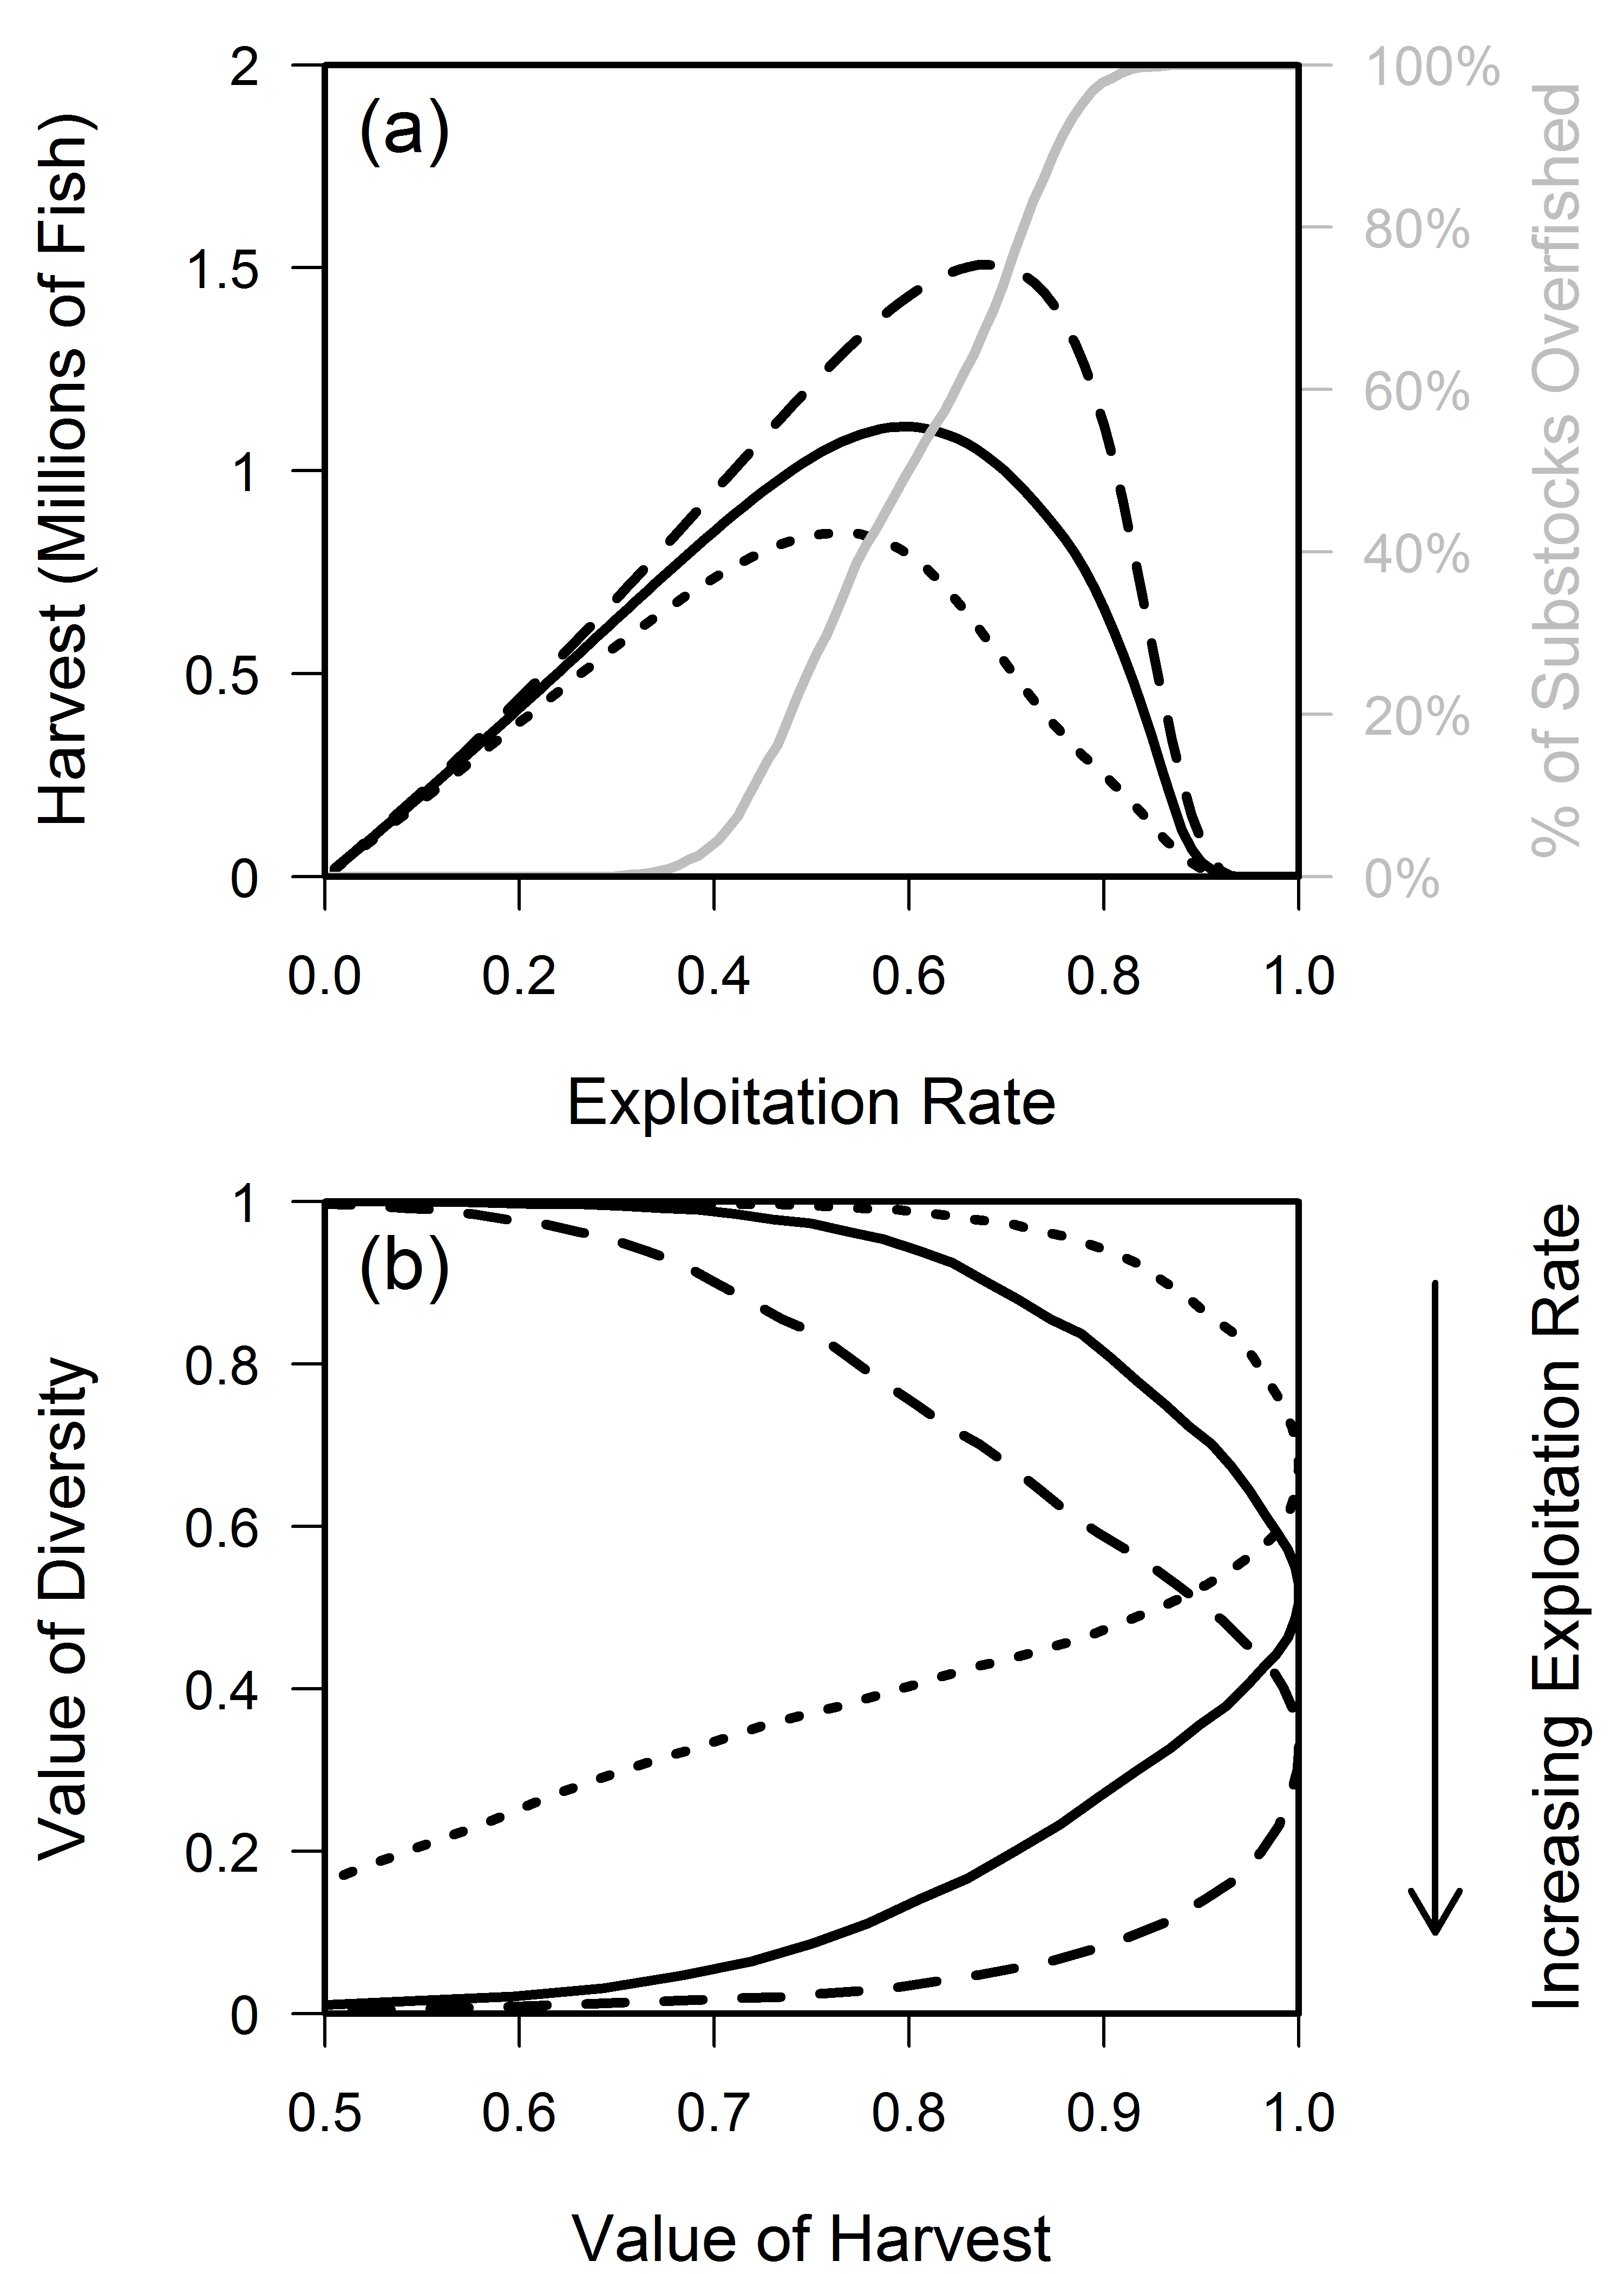
\includegraphics{img/Ch4/trade-off-plot.png}
  \caption{Visualization of how different types of hetergeneity in substock productivity and size influence the shape of trade-offs in mixed-stock salmon fisheries. Solid black likes are the case where stock types are split evenly among large/small and productive/unproductive stocks. Dotted black likes are the case where all small stocks are productive and all large stocks are unproductive, and dashed lines are the opposite (i.e., all big stocks are productive). (\textit{a}) Equilibrium aggregate harvest and proportion of substocks overfished plotted against the exploitation rate (\textit{b}) value of the biodiversity objective (0 = all stocks overfished) plotted against the value of harvest (the long term proportion of the aggregate MSY attained). Notice that when all big stocks are productive (dashed lines), the trade-off is steeper, i.e., more harvest must be sacrificed in order to ensure a greater fraction of substocks are not overfished. }
  \label{fig:trade-off-plot}
\end{figure}

\clearpage
\pagestyle{plain}

\begin{figure}
  \centering
  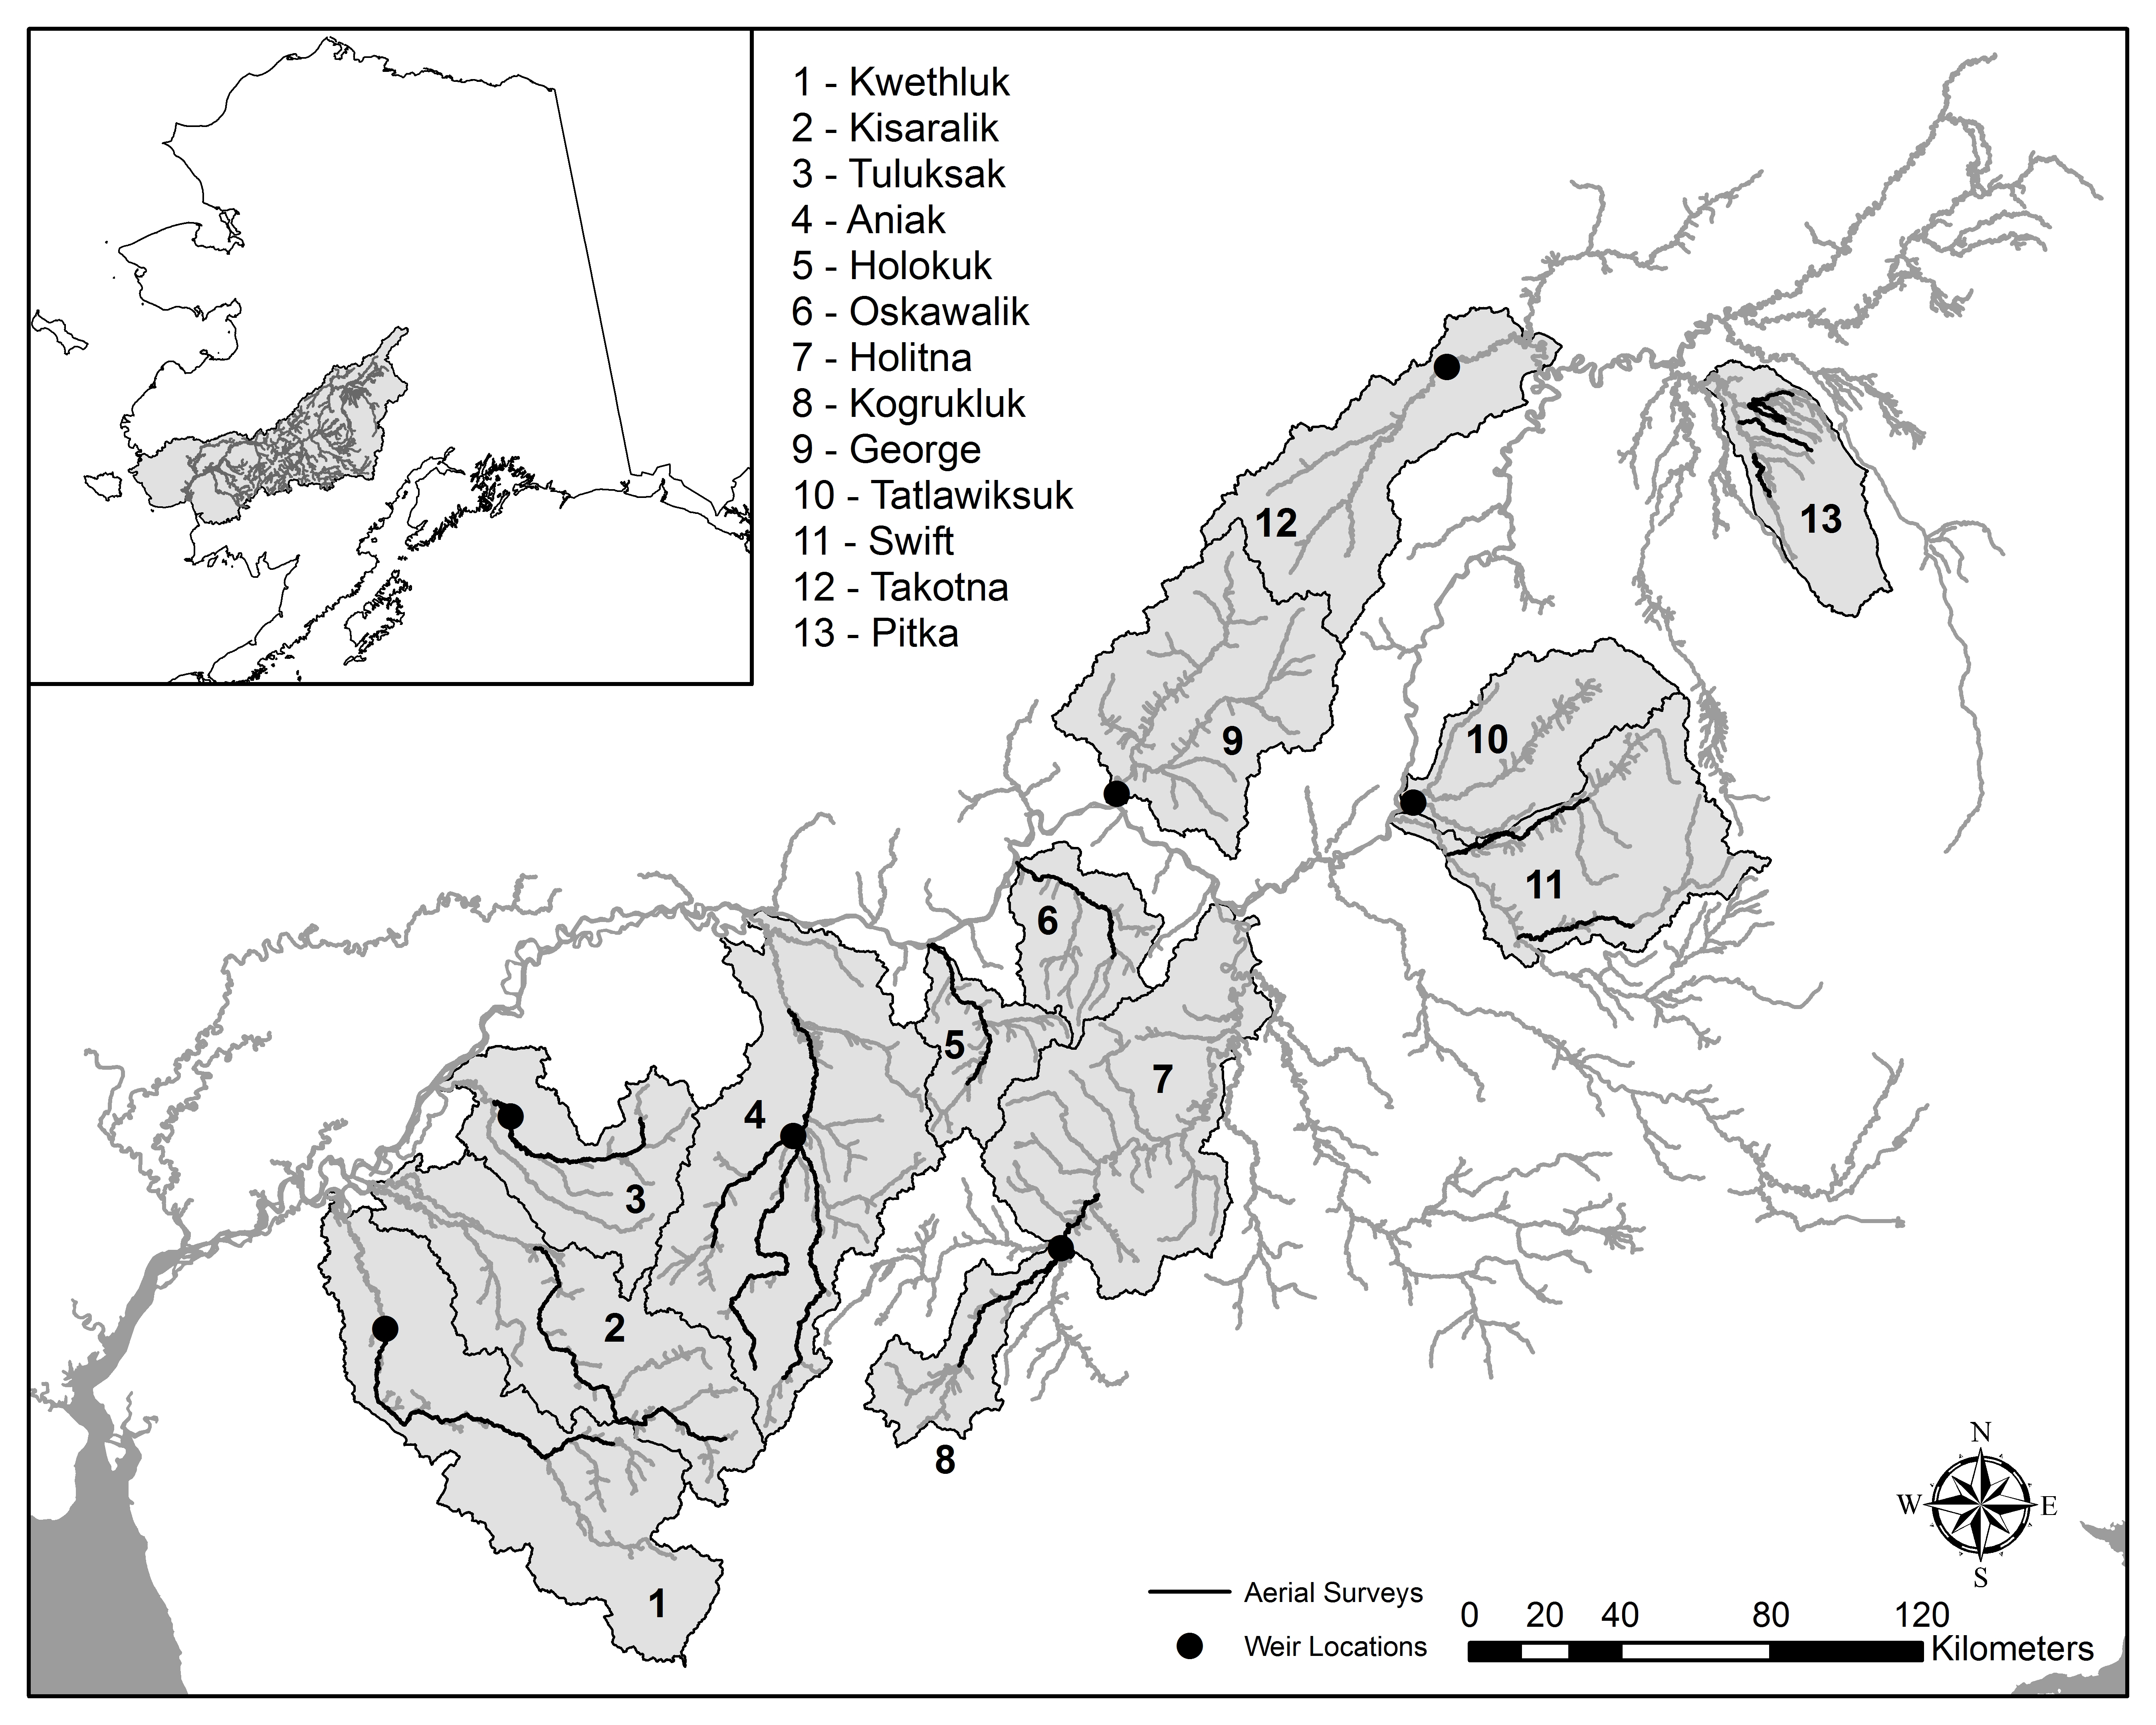
\includegraphics{img/Ch4/ch4-map.jpg}
  \caption{Map of the Kuskokwim River drainage, with the 13 drainage basins representing unique spawning units (substocks) used in this analysis. Black points show the location of weir projects, black sections of river indicate the reaches flown as part of aerial surveys. Drainages monitored via both aerial survey and weir used the weir counts to inform escapement estimates in this analysis, with the exception of the Aniak drainage (4), for which aerial survey data were much more abundant than the weir data.}
  \label{fig:ch4-map}
\end{figure}

\clearpage

\begin{figure}
  \centering
  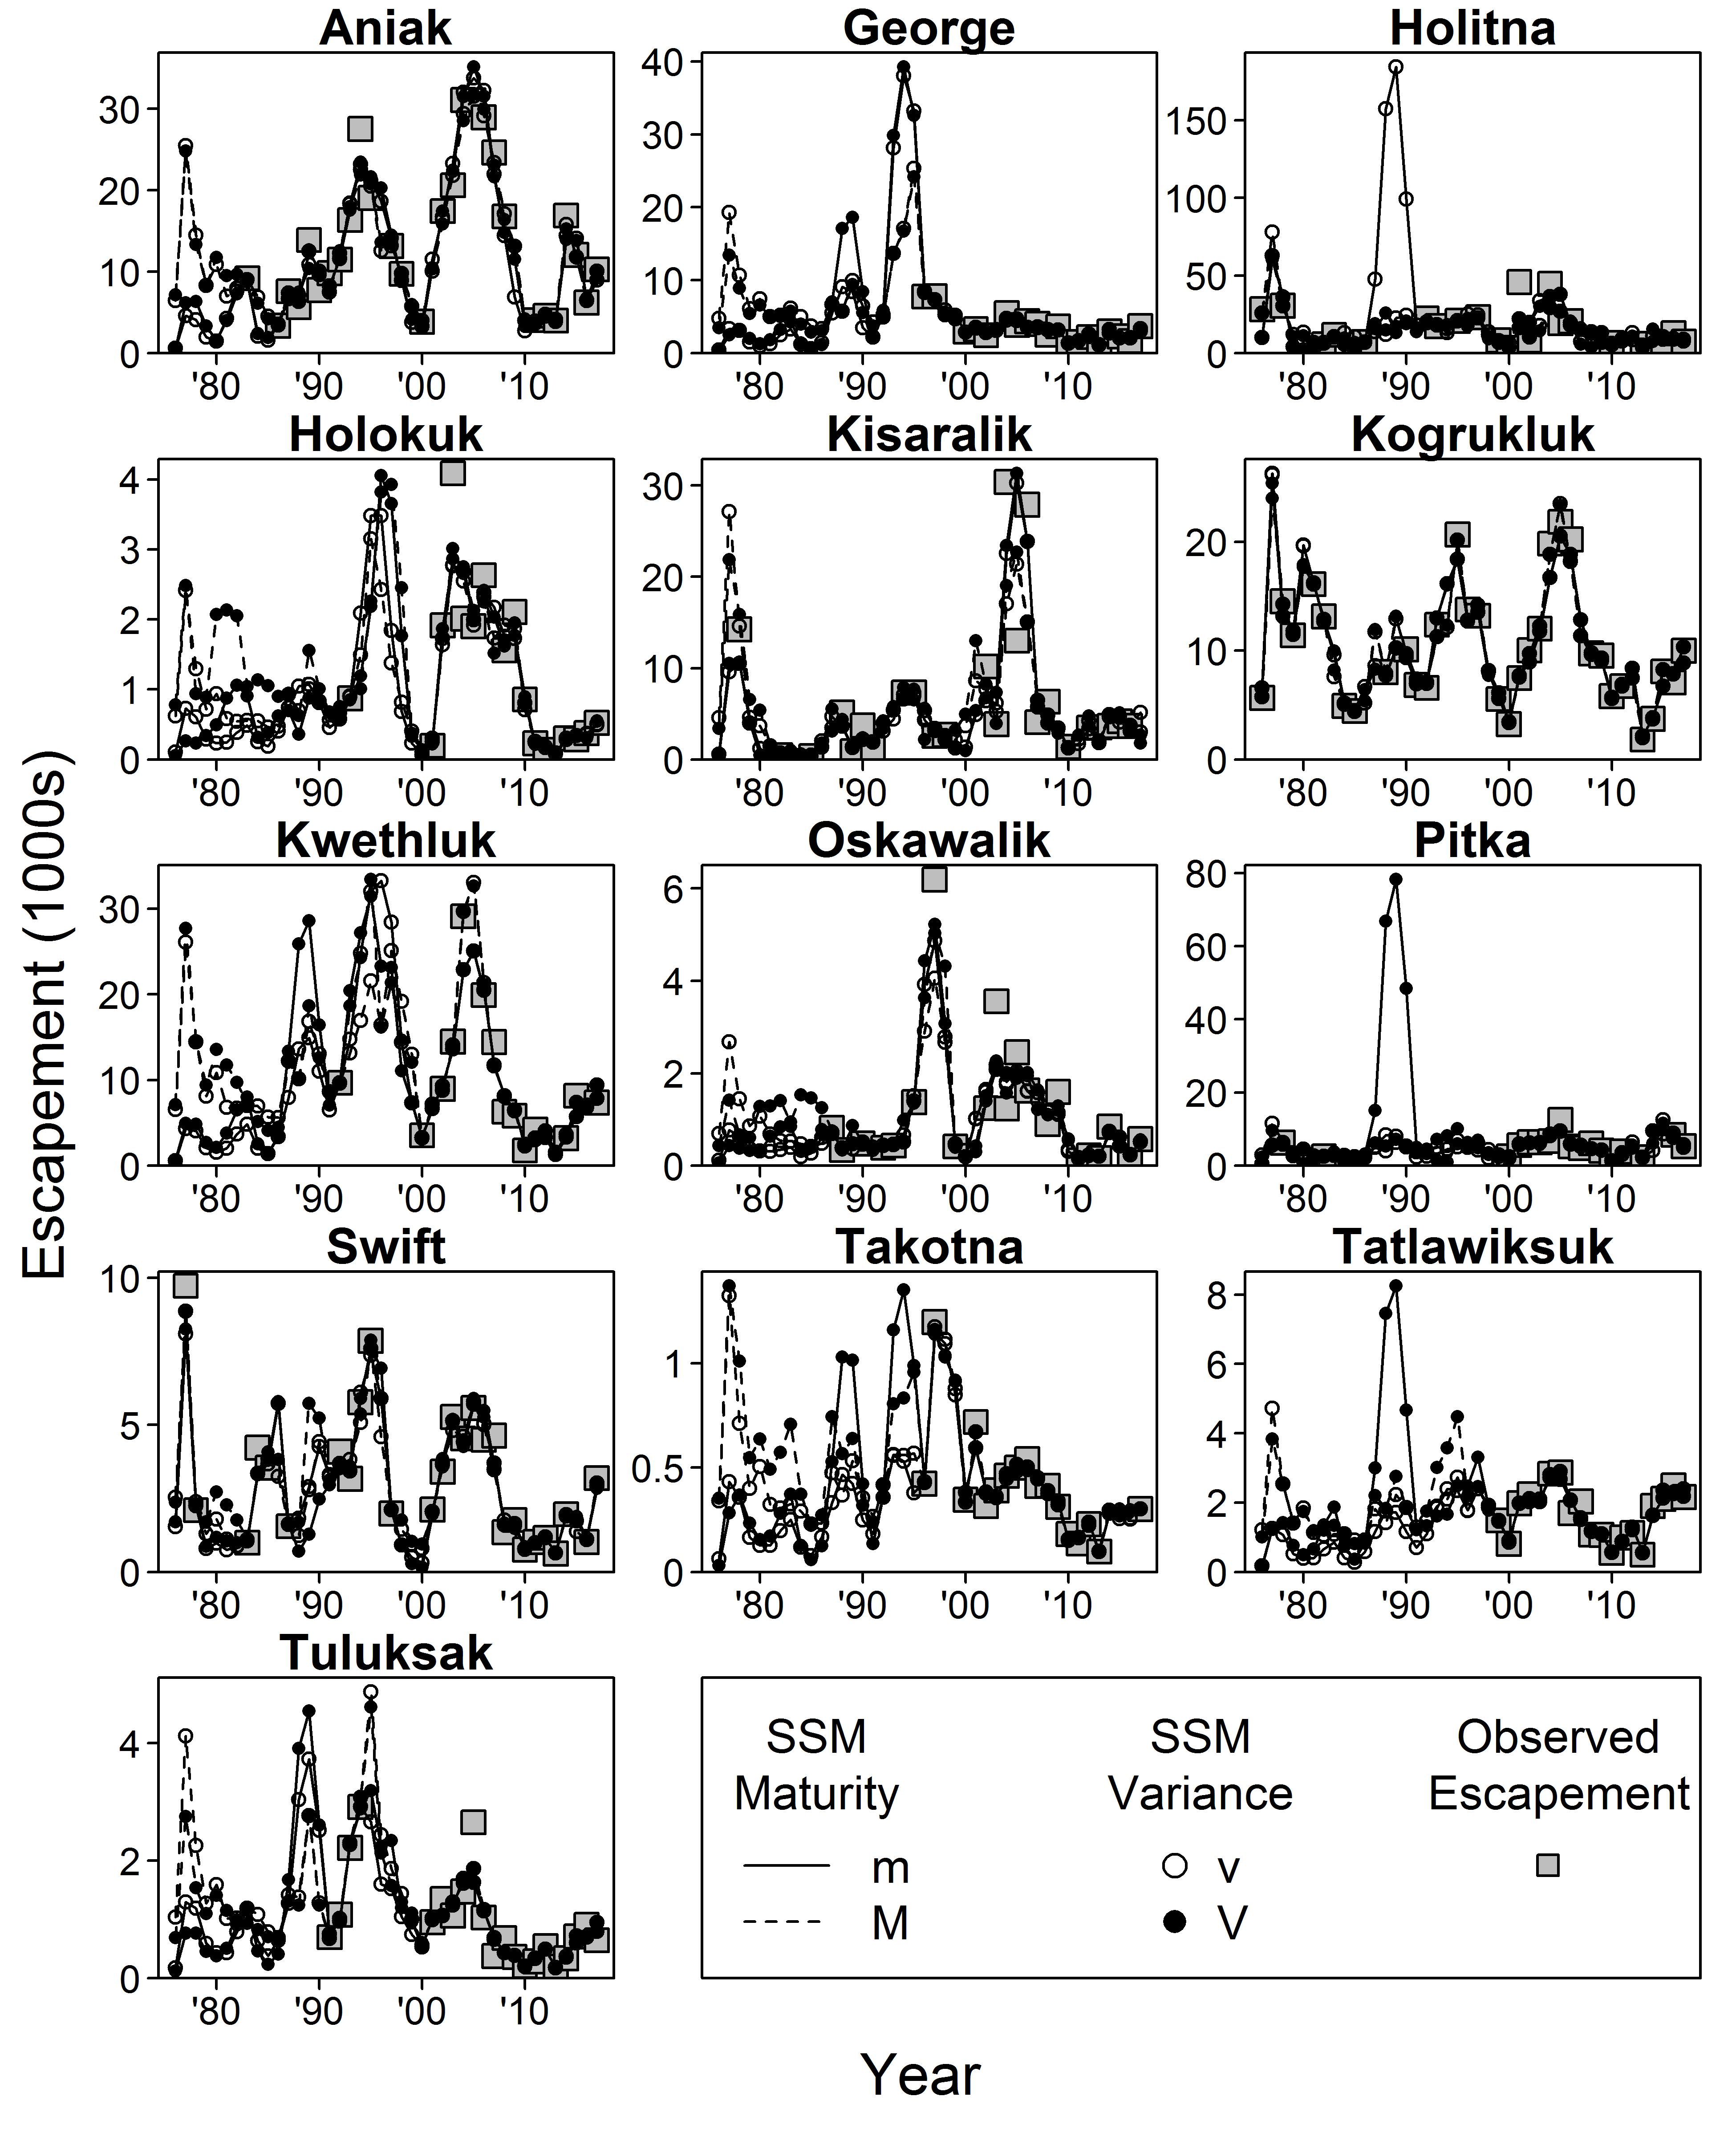
\includegraphics{img/Ch4/S-fit.jpg}
  \caption{Observed and fitted escapement time series for each Kuskokwim River substock. Line/symbol types denote the particular state-space model and grey squares denote observed data.}
  \label{fig:S-fit}
\end{figure}

\clearpage

\begin{figure}
  \centering
  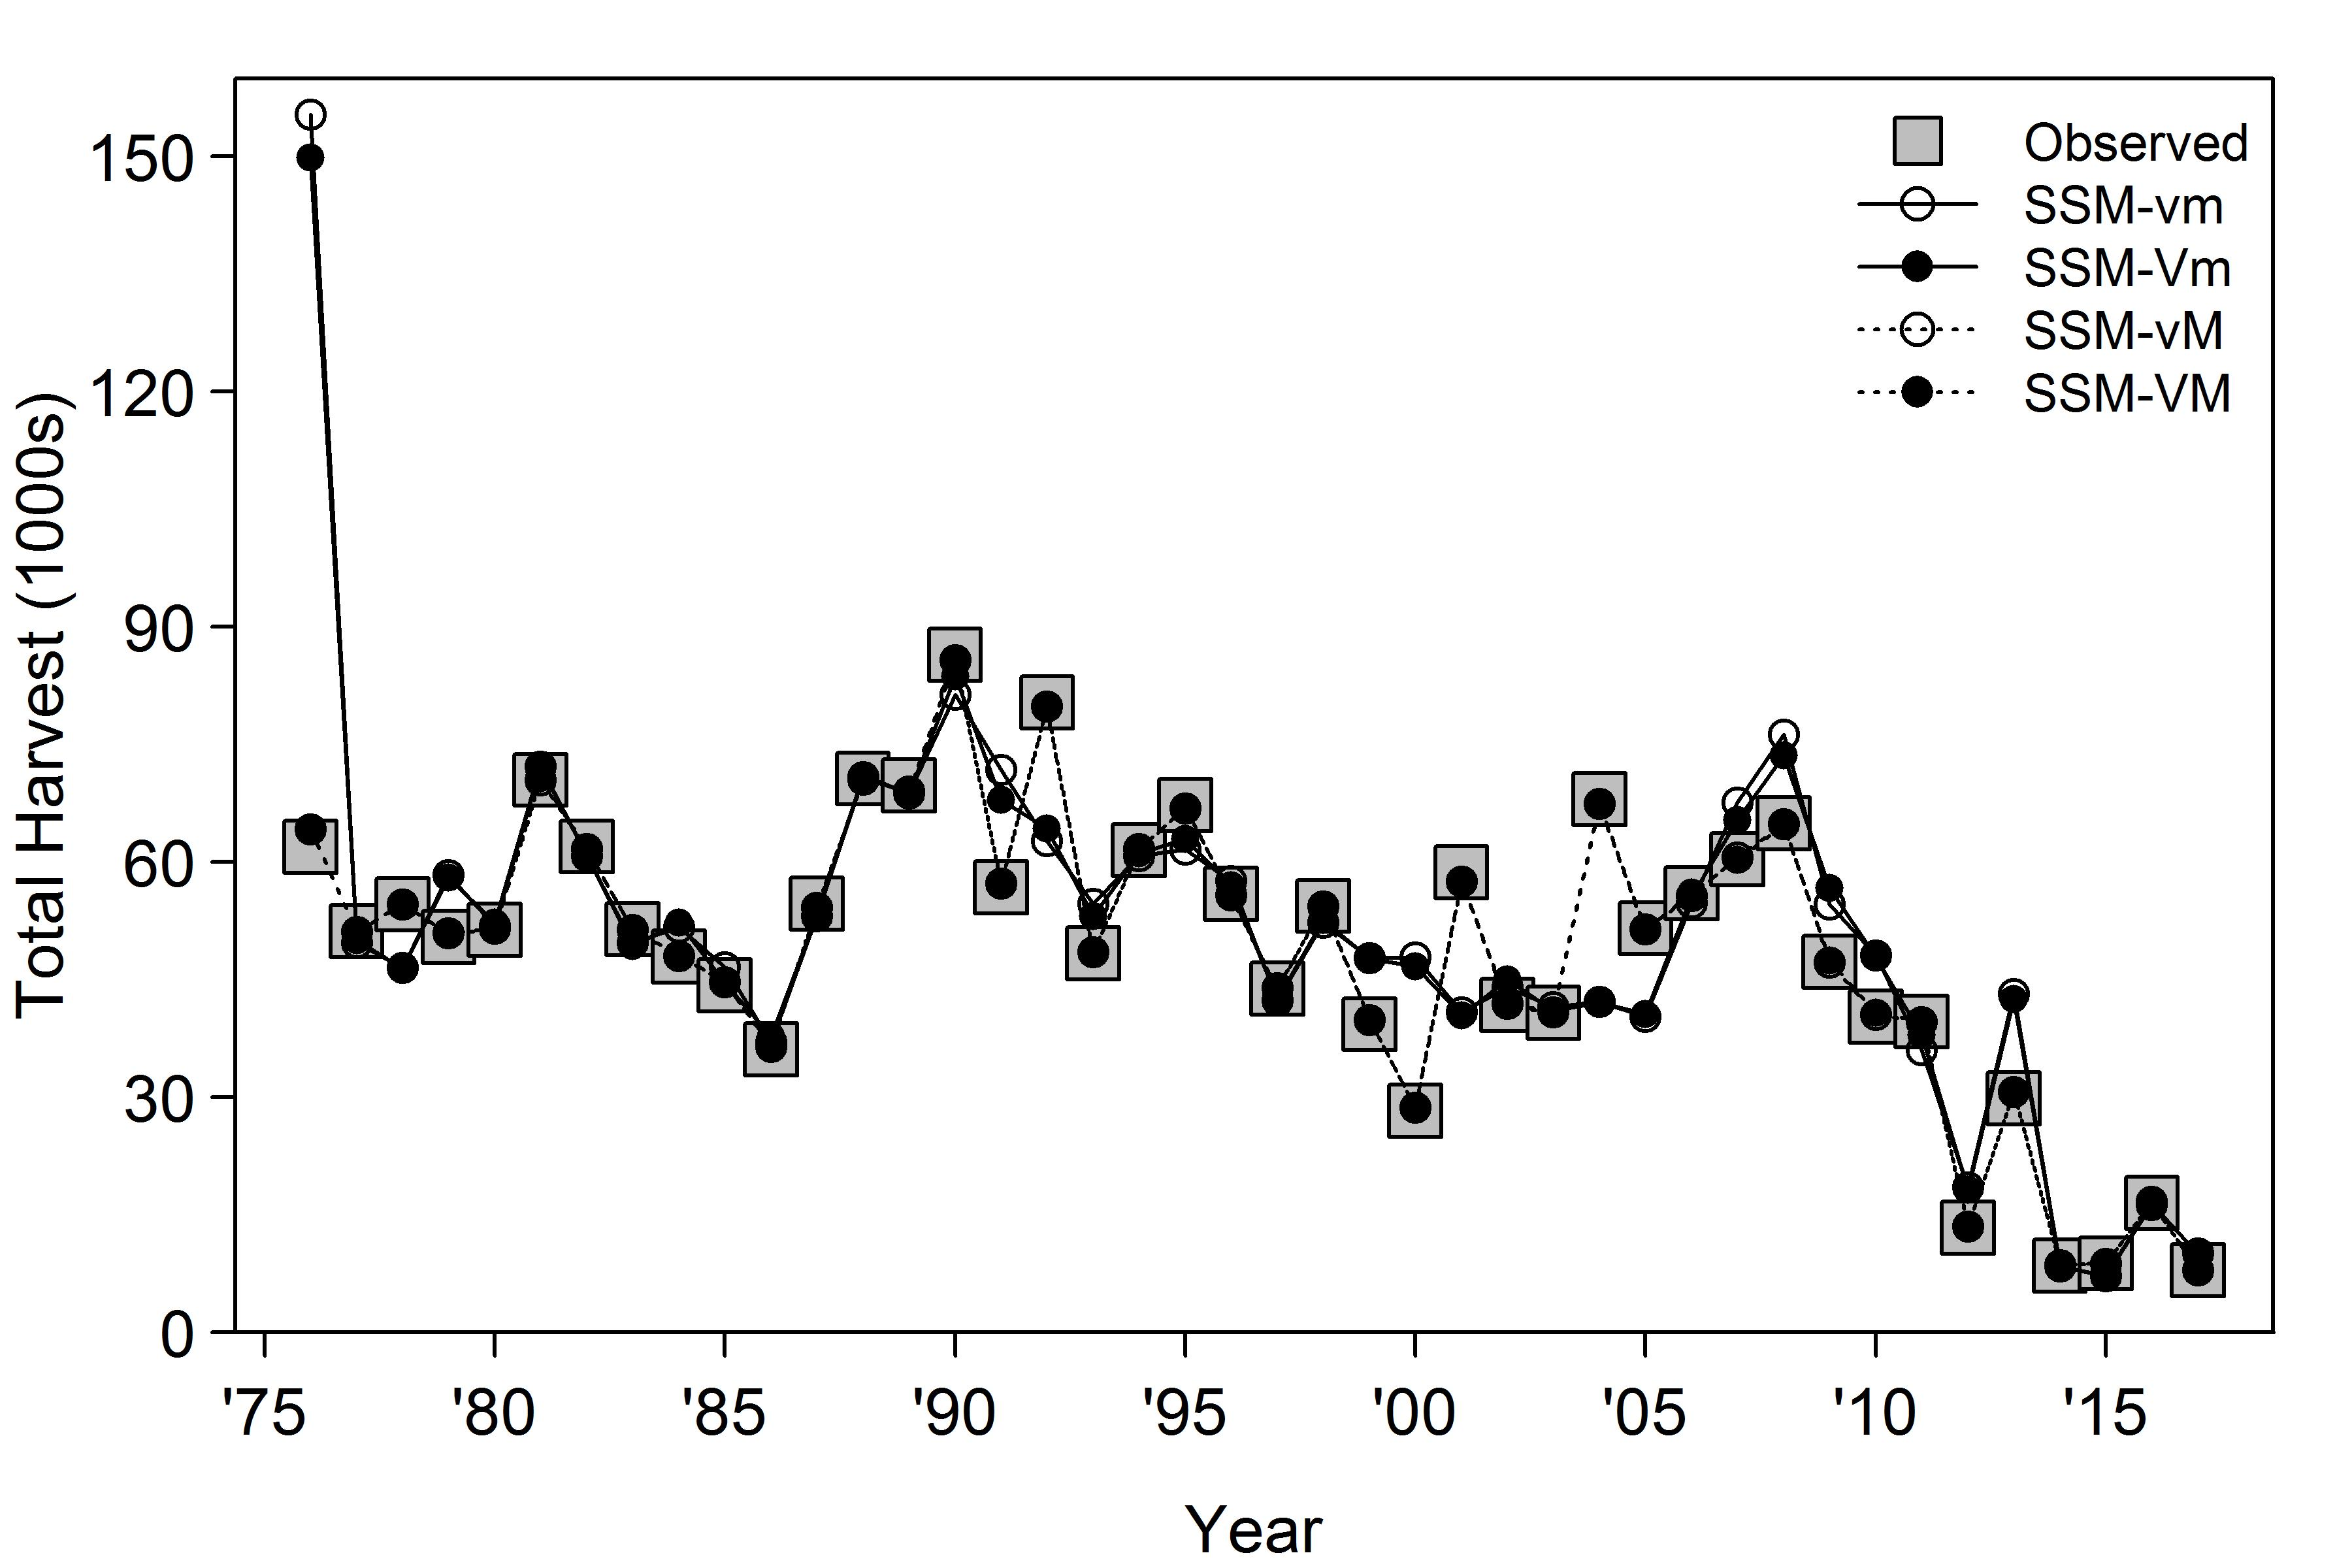
\includegraphics{img/Ch4/H-fit.jpg}
  \caption{Observed and fitted harvest time series aggregated across all Kuskokwim River substocks included in this analysis. Line/symbol types denote the particular state-space model and grey squares denote observed data.}
  \label{fig:H-fit}
\end{figure}

\clearpage

\begin{figure}
  \centering
  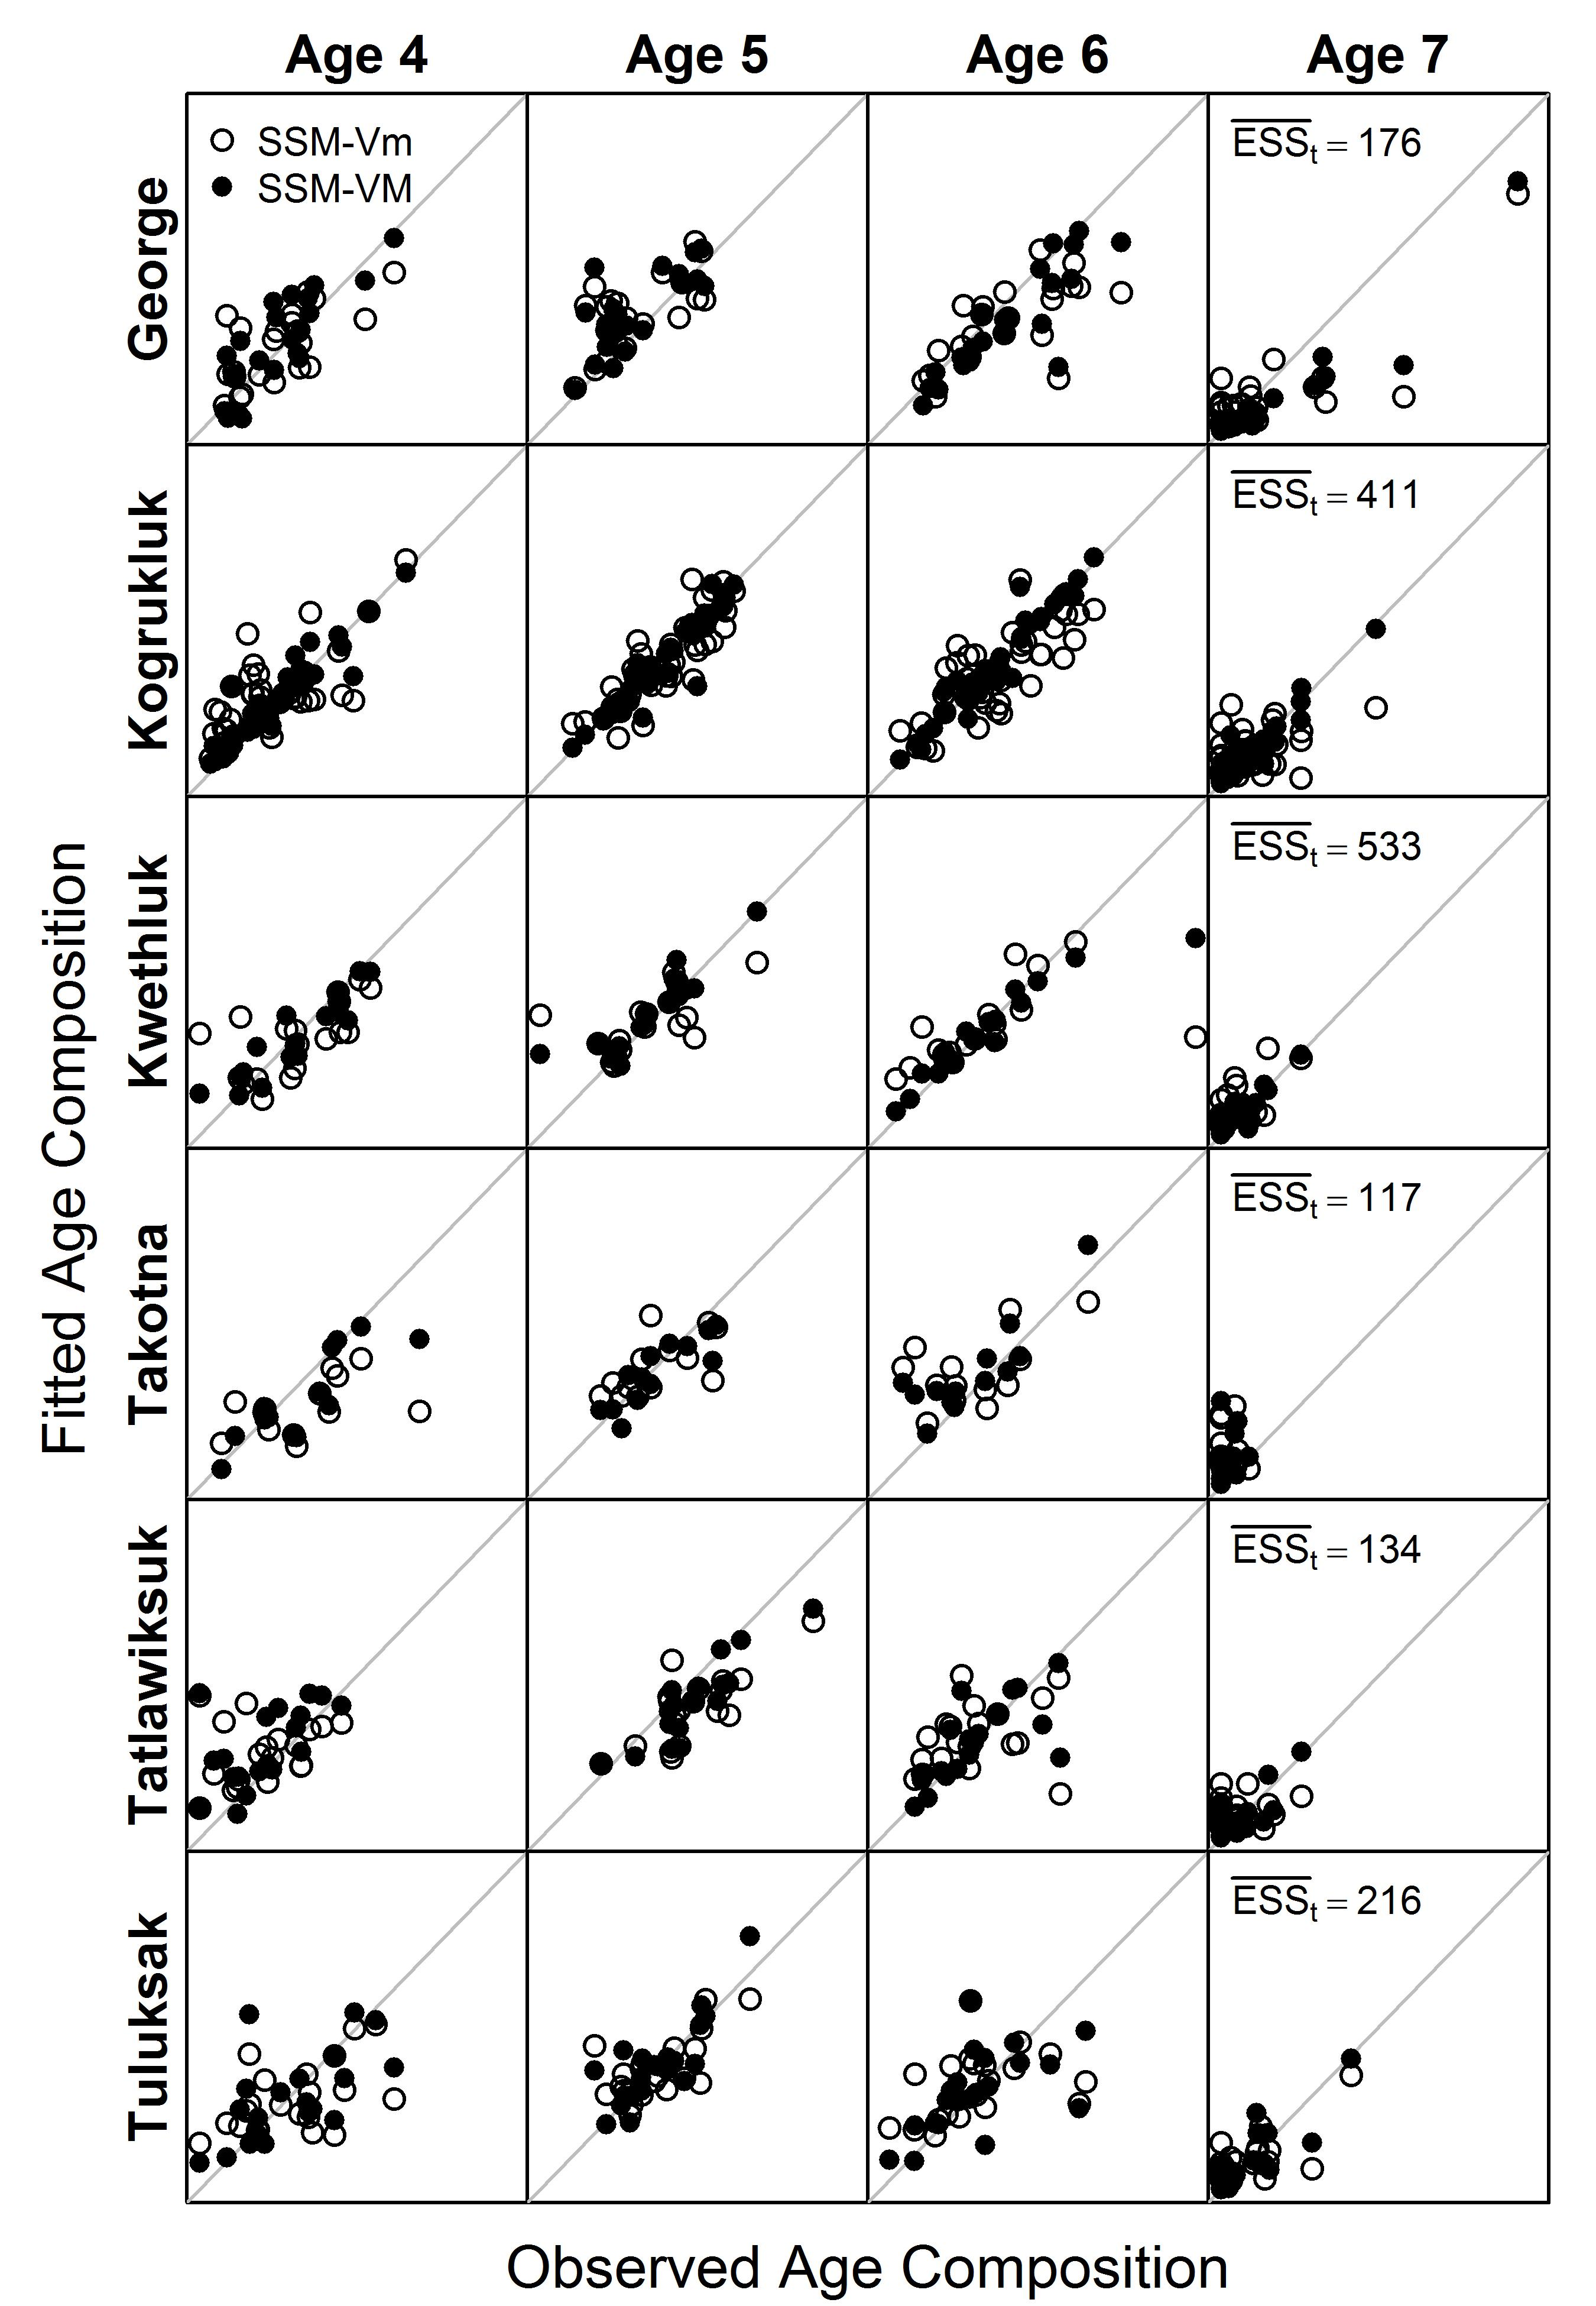
\includegraphics{img/Ch4/age-fit.jpg}
  \caption{Observed and fitted age composition for the 6 weir-monitored substocks. Each scatter plot is the pair of fitted \textit{versus} observed proportion of the escapement in each age each year with data available and the grey line represents the 1:1 perfect fit line. Point types denote two models: SSM-Vm (time-constant maturity; hollow circles) and SSM-VM (time-varying maturity; filled circles). $\overline{ESS}_t$ represents the average number of fish successfully aged each year with data for each substock, which was used as the sample size to weight the data in the multinomial likelihoods that used these data. Panels are scaled to have the same \textit{x}-axis and \textit{y}-axis limits within an age across substocks and range from 0 -- 1 for ages 4 -- 6 and 0 -- 0.3 for age 7.}
  \label{fig:age-fit}
\end{figure}

\clearpage
\pagestyle{empty}

\begin{figure}
  \centering
  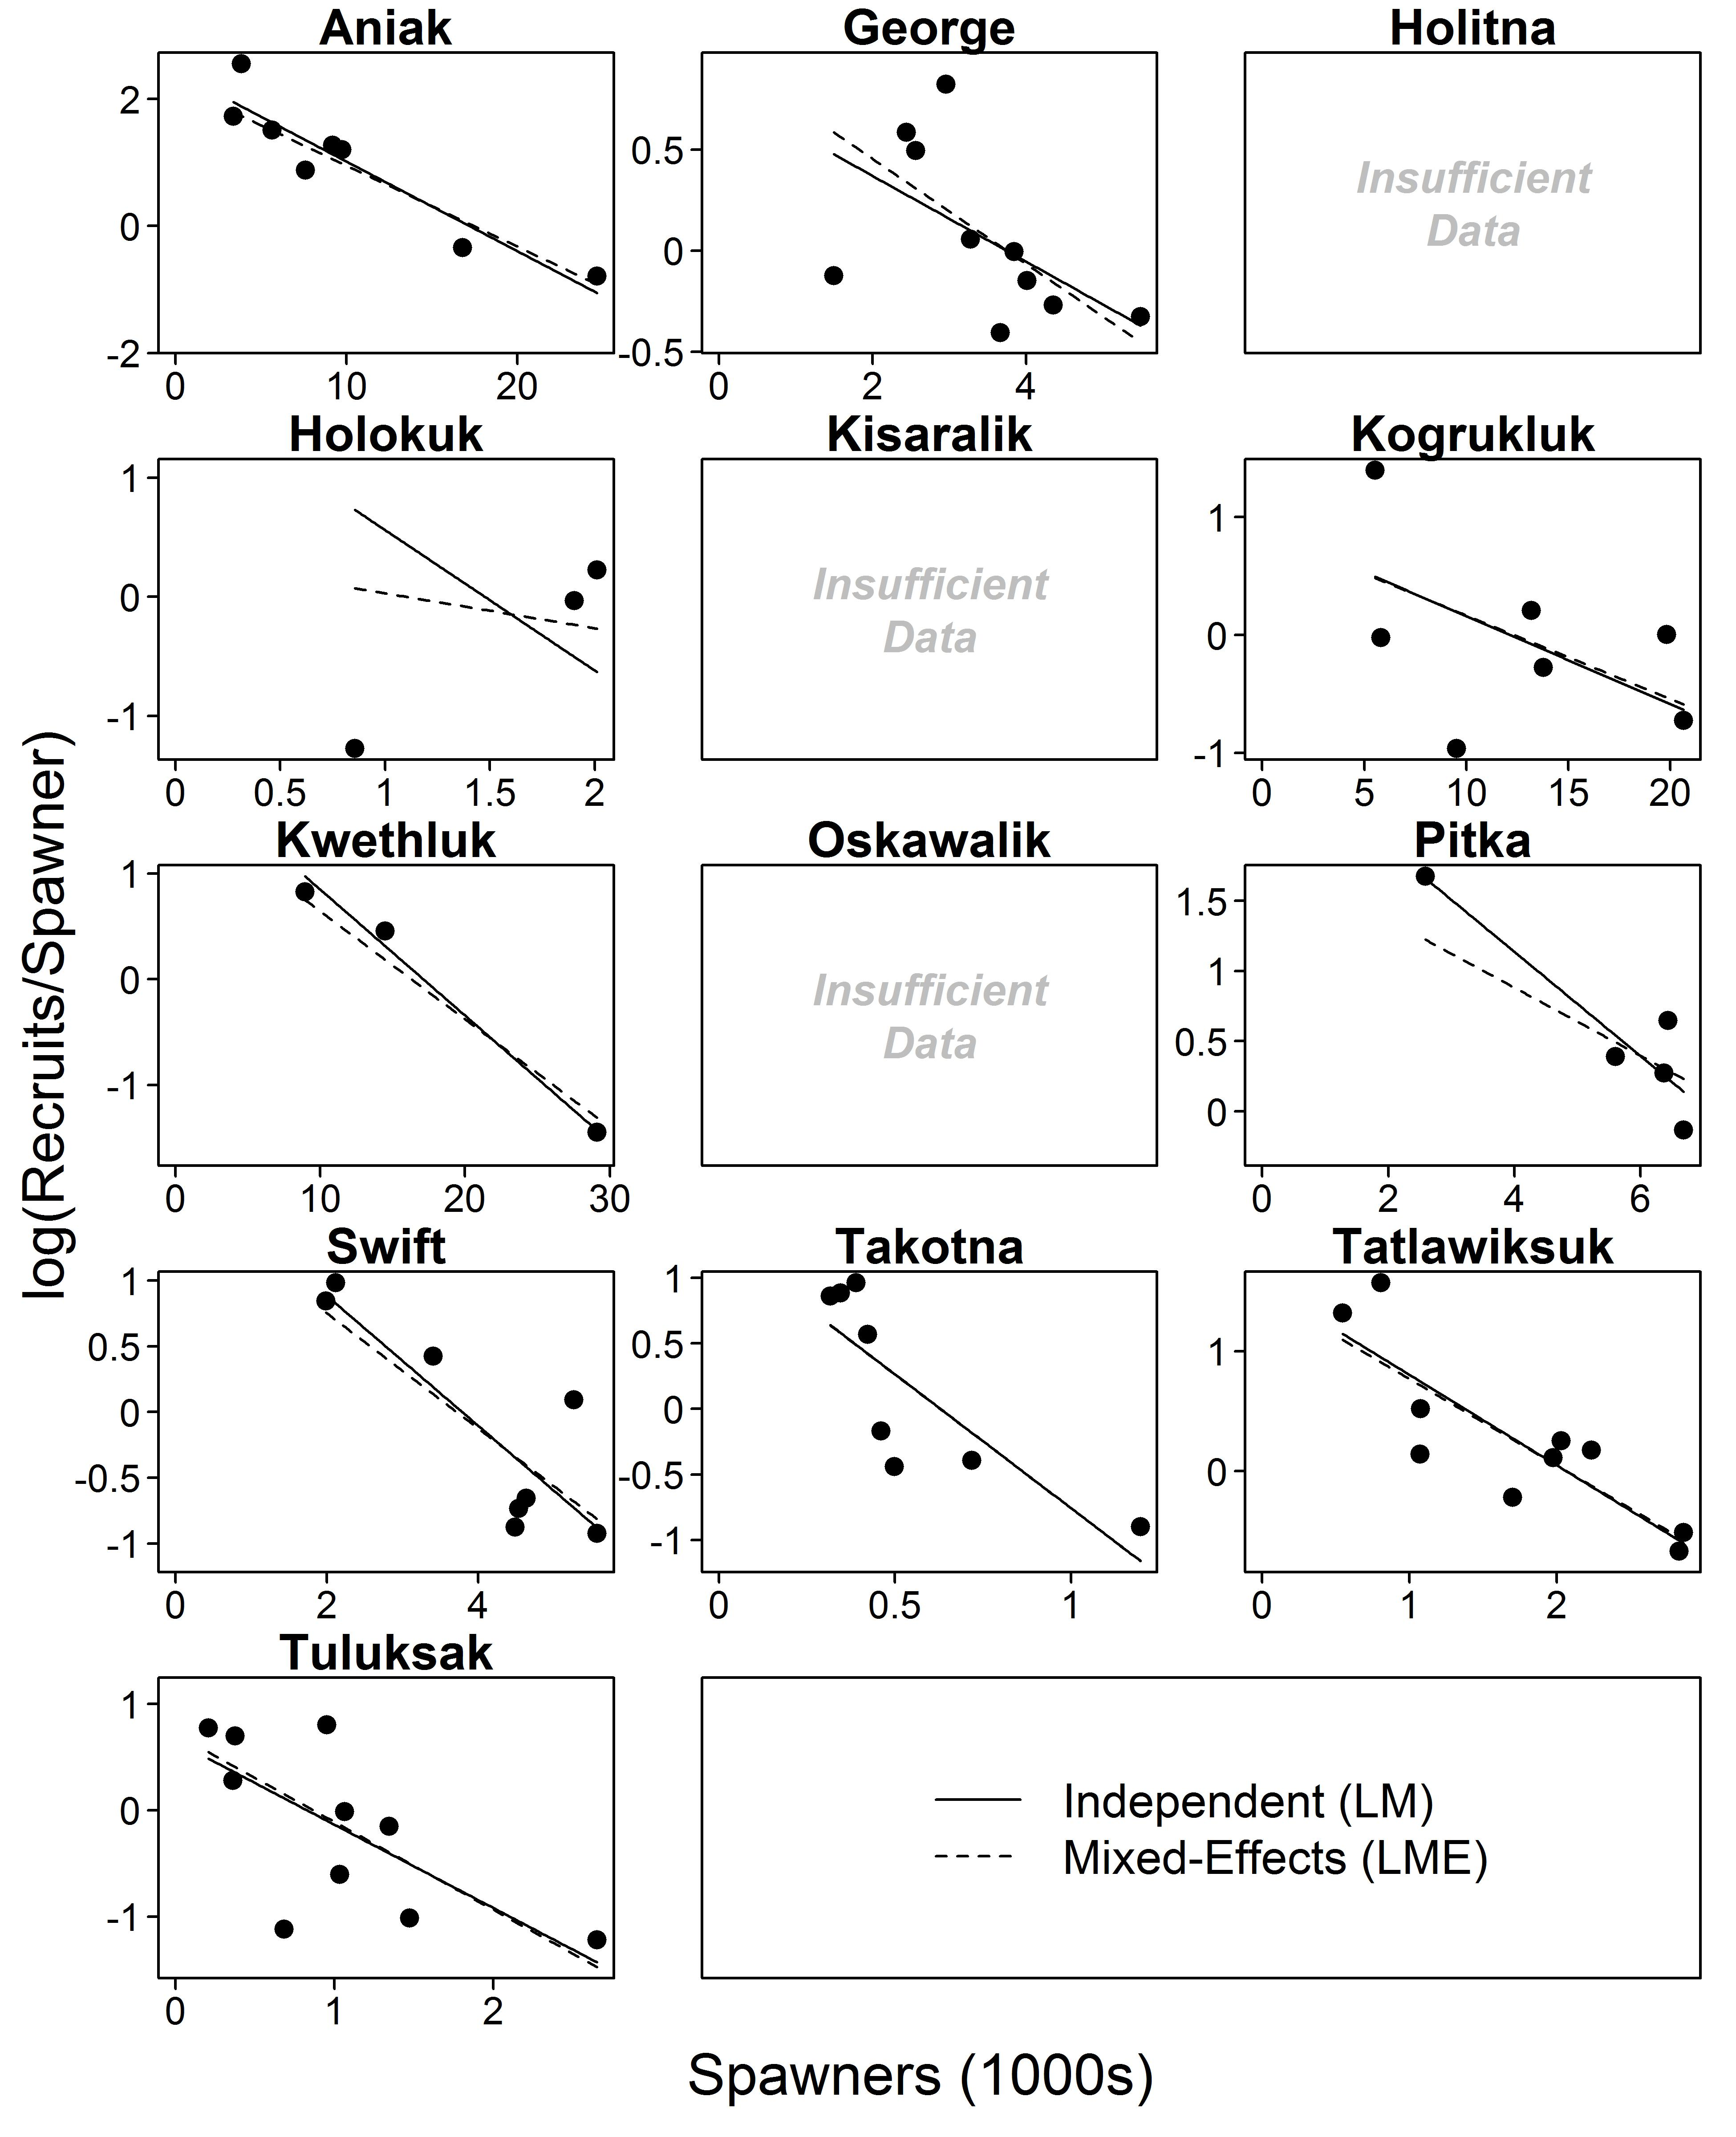
\includegraphics{img/Ch4/RPS-v-S.jpg}
  \caption{Fit of the regression approaches to fitting the multi-stock spawner-recruit analysis to the Kuskokwim River substock data. Points are observed log(recruits/spawner) \textit{versus} spawners, solid lines represent the fit for the independent regression models, and dashed lines represent the fit suggested by the model with random intercept effects for each substocks. Three substocks had fewer than 3 observed data points, rendering fitting a regression line infeasible. Note that a constraint was imposed that maintained $\log(\alpha_{j}) > 0$ which prevented biologically implausible values, and explains the poor fit for the Holokuk River substock.}
  \label{fig:rps-v-s}
\end{figure}

\clearpage

\begin{figure}
  \centering
  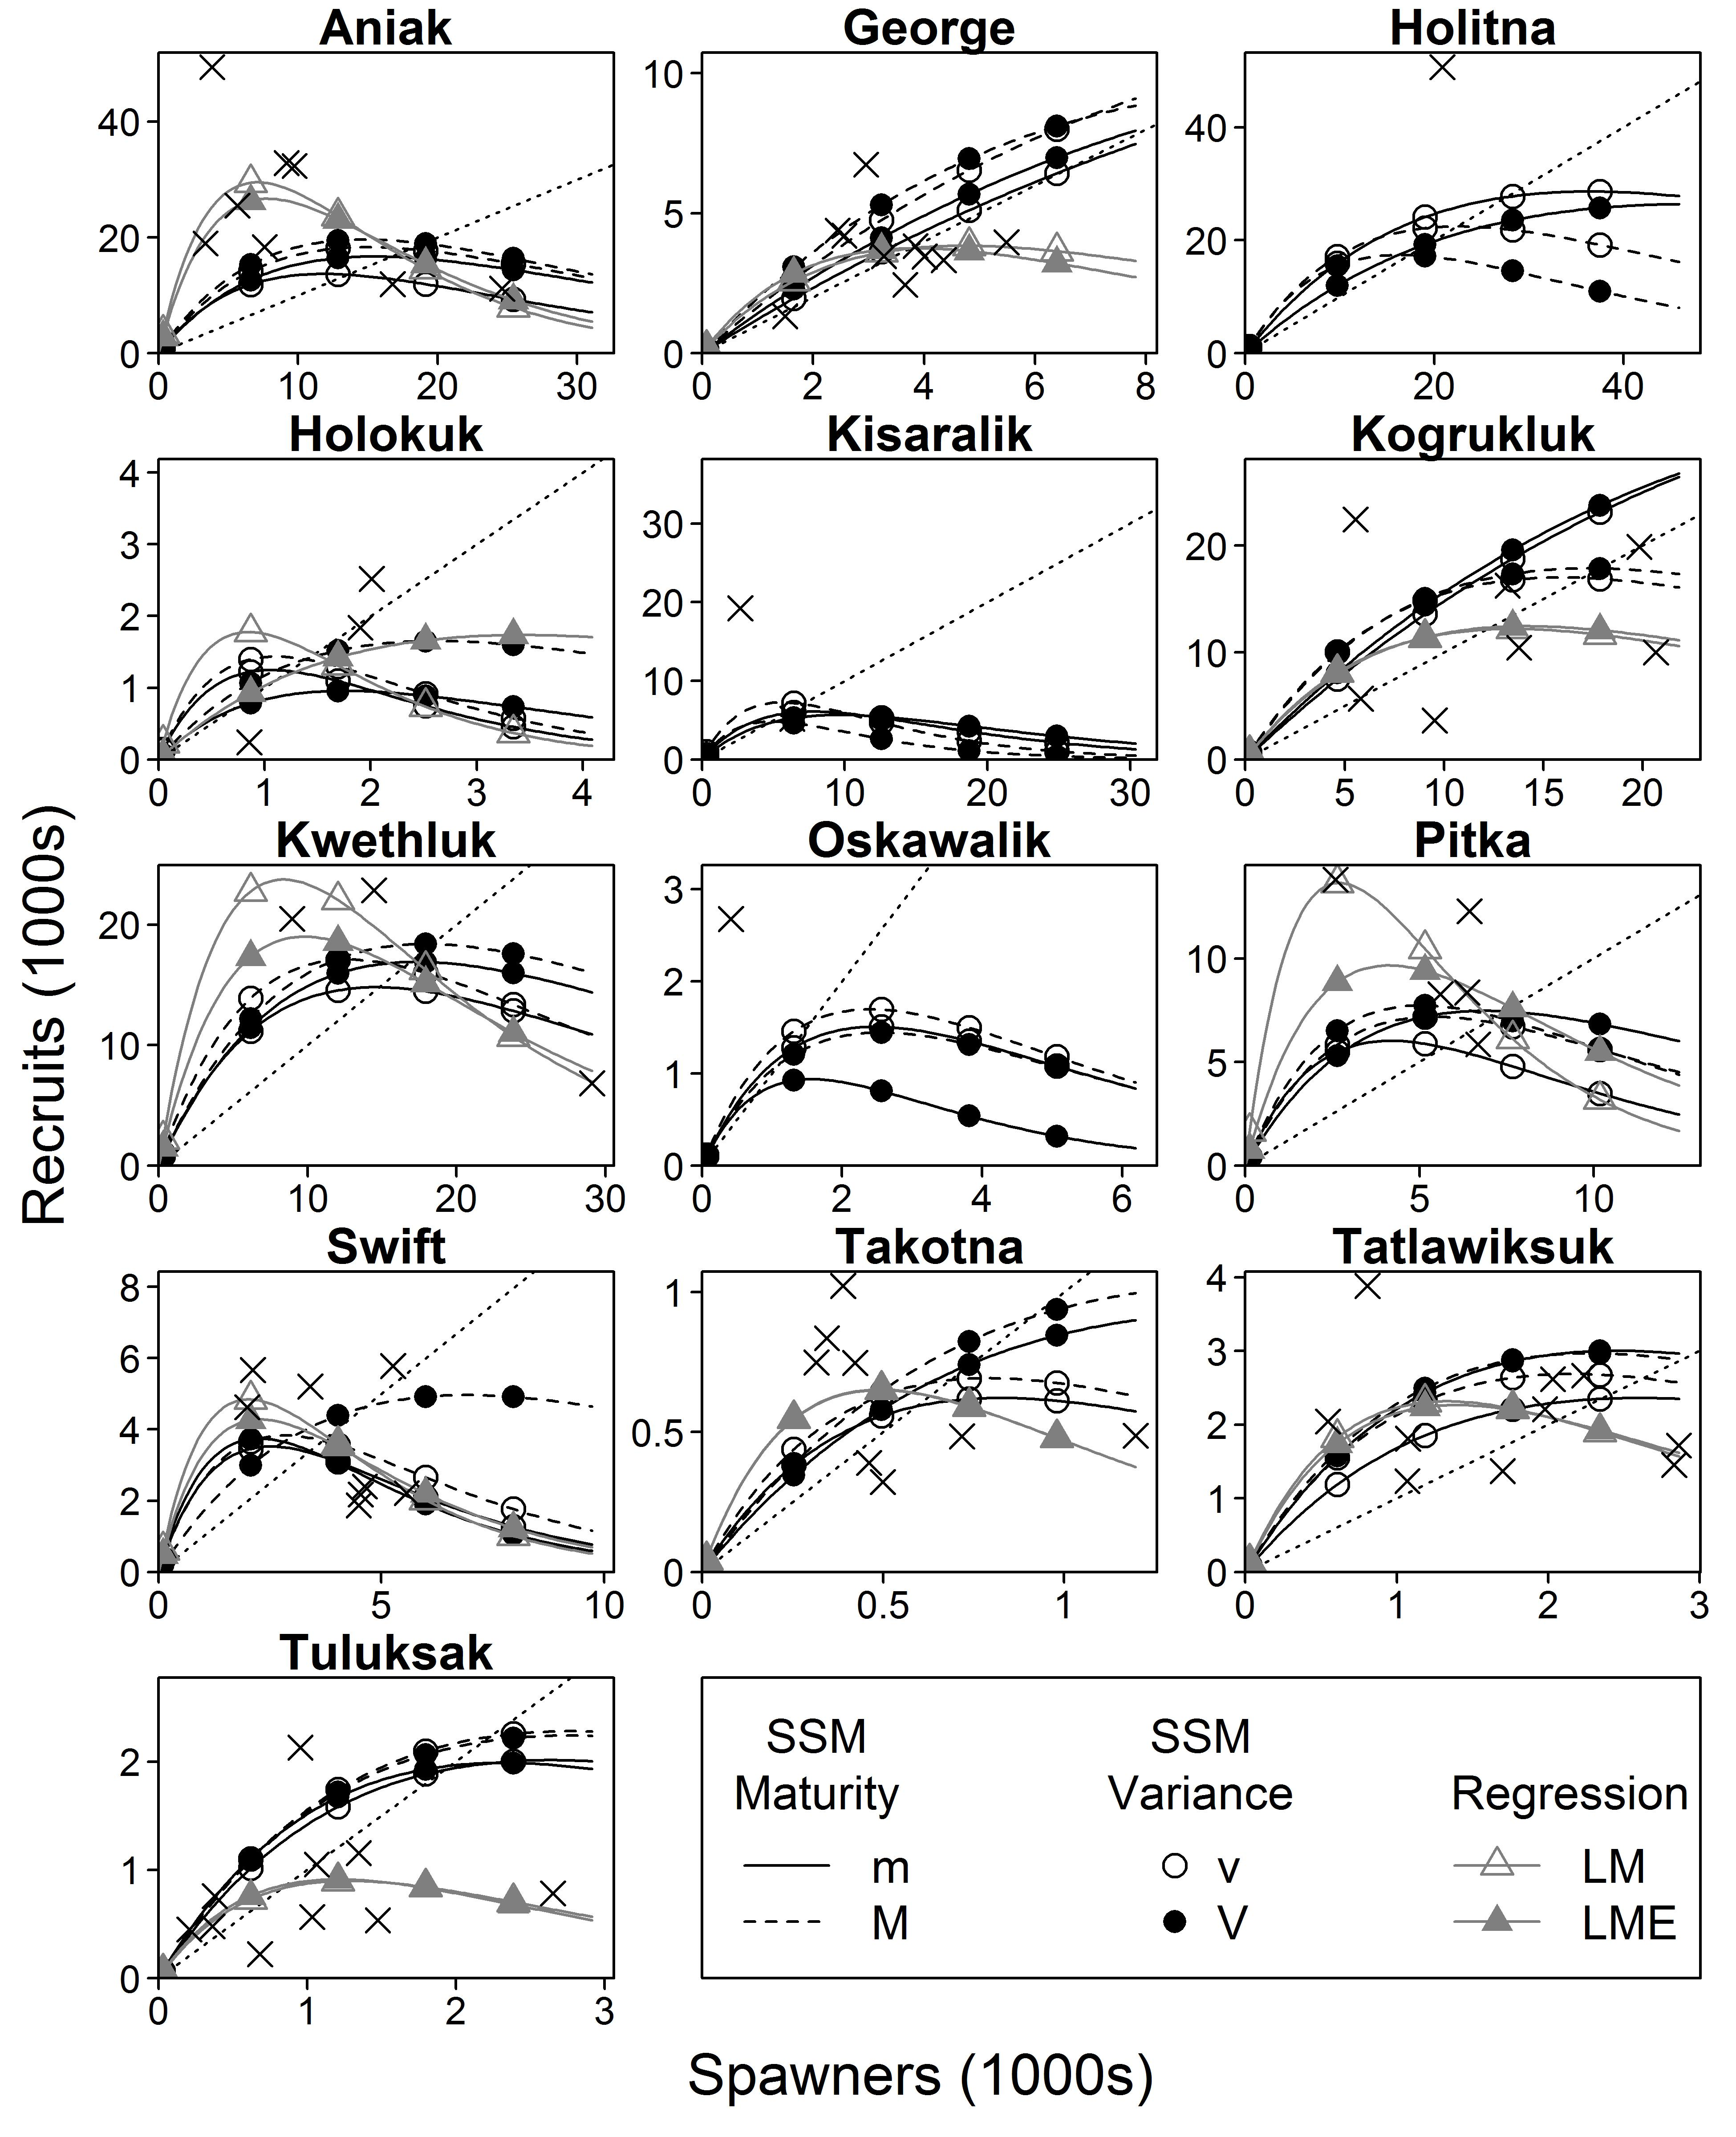
\includegraphics{img/Ch4/R-v-S.jpg}
  \caption{Fitted spawner-recruit relationships for the 13 substocks monitored in the Kuskokwim River subdrainage included in this analysis. Line and point types correspond to different models; crosses are completely-observed spawner-recruit pairs. Note that the regression approaches (grey lines/triangles) fitted only to these data, the state-space models (black lines/circles) fitted to all observations of substock-specific escapement, aggregate harvest, and age composition.}
  \label{fig:r-v-s}
\end{figure}

\clearpage
\pagestyle{plain}

\begin{figure}
  \centering
  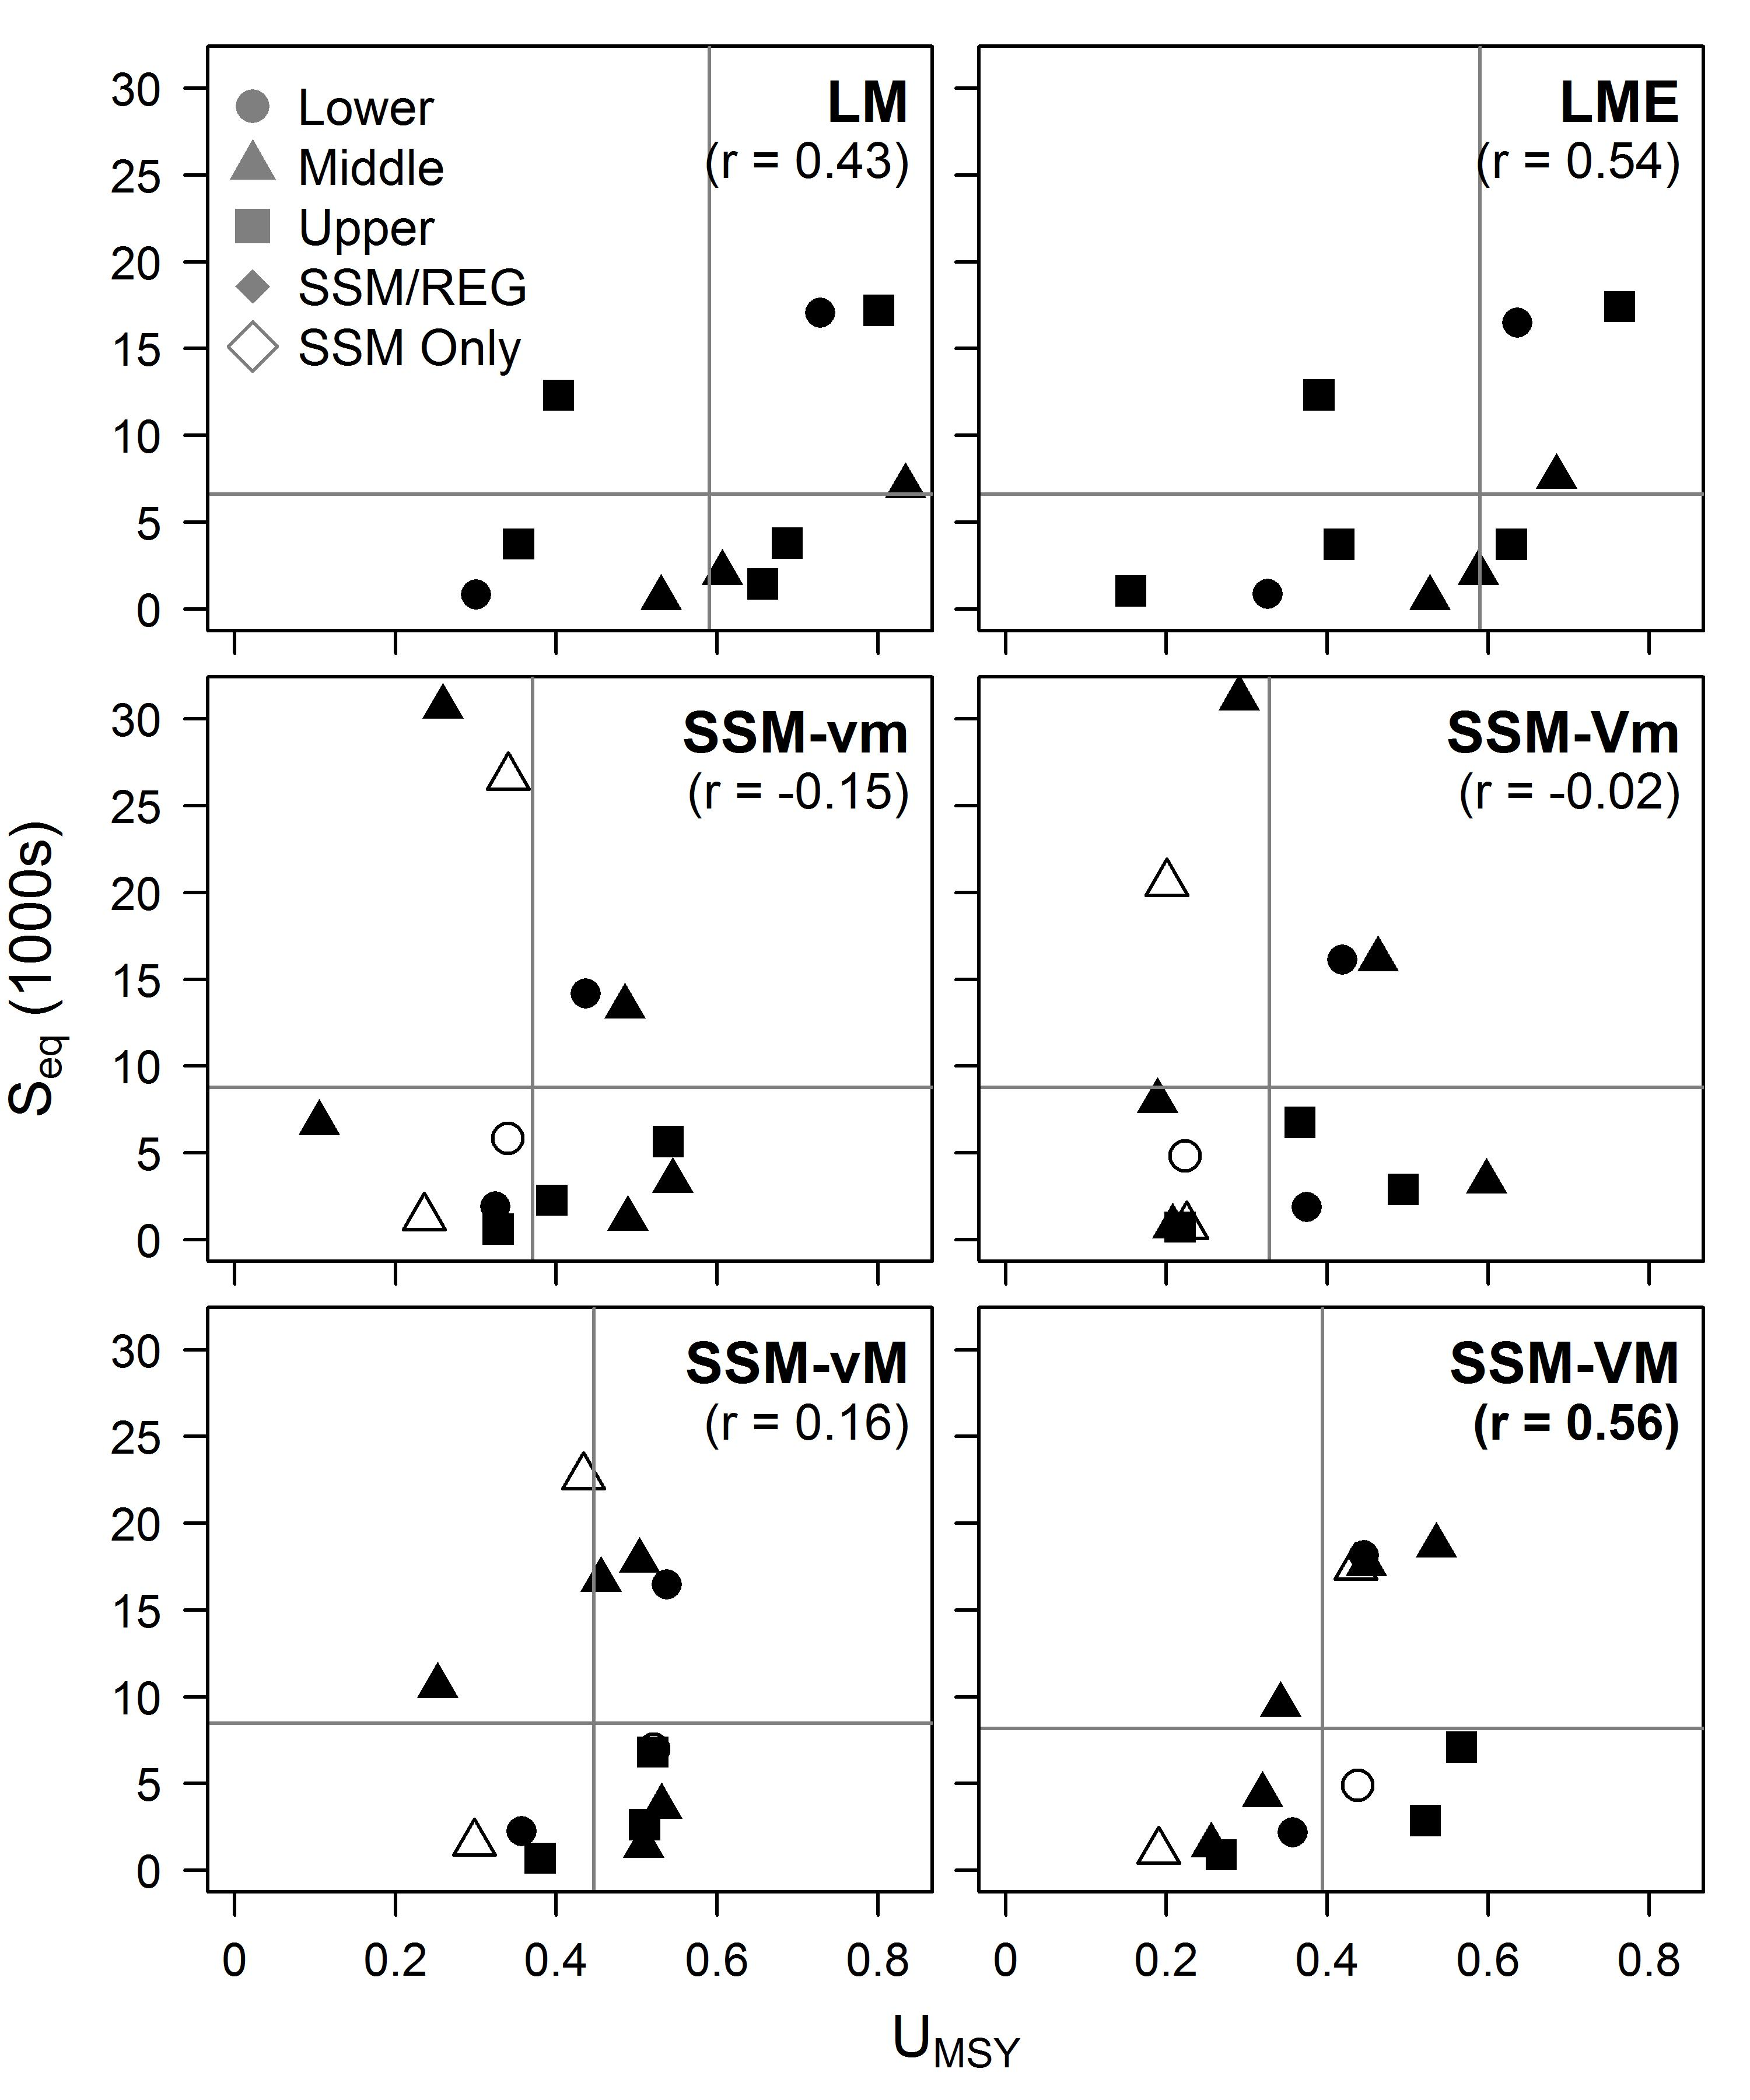
\includegraphics{img/Ch4/Size-v-Prod.jpg}
  \caption{Relationships between substock size and productivity as estimated by the 6 estimation approaches in the analysis. Symbol shapes denote the region within the Kuskokwim drainage the substock is located in and hollow symbols in the state-space models are substocks that could not be fitted by the regression approaches. The value in parentheses is Pearson's $r$ correlation coefficient; bold numbers indicate a signficant correlation at $\alpha$ = 0.05.}
  \label{fig:size-v-prod}
\end{figure}

\clearpage

\begin{figure}
  \centering
  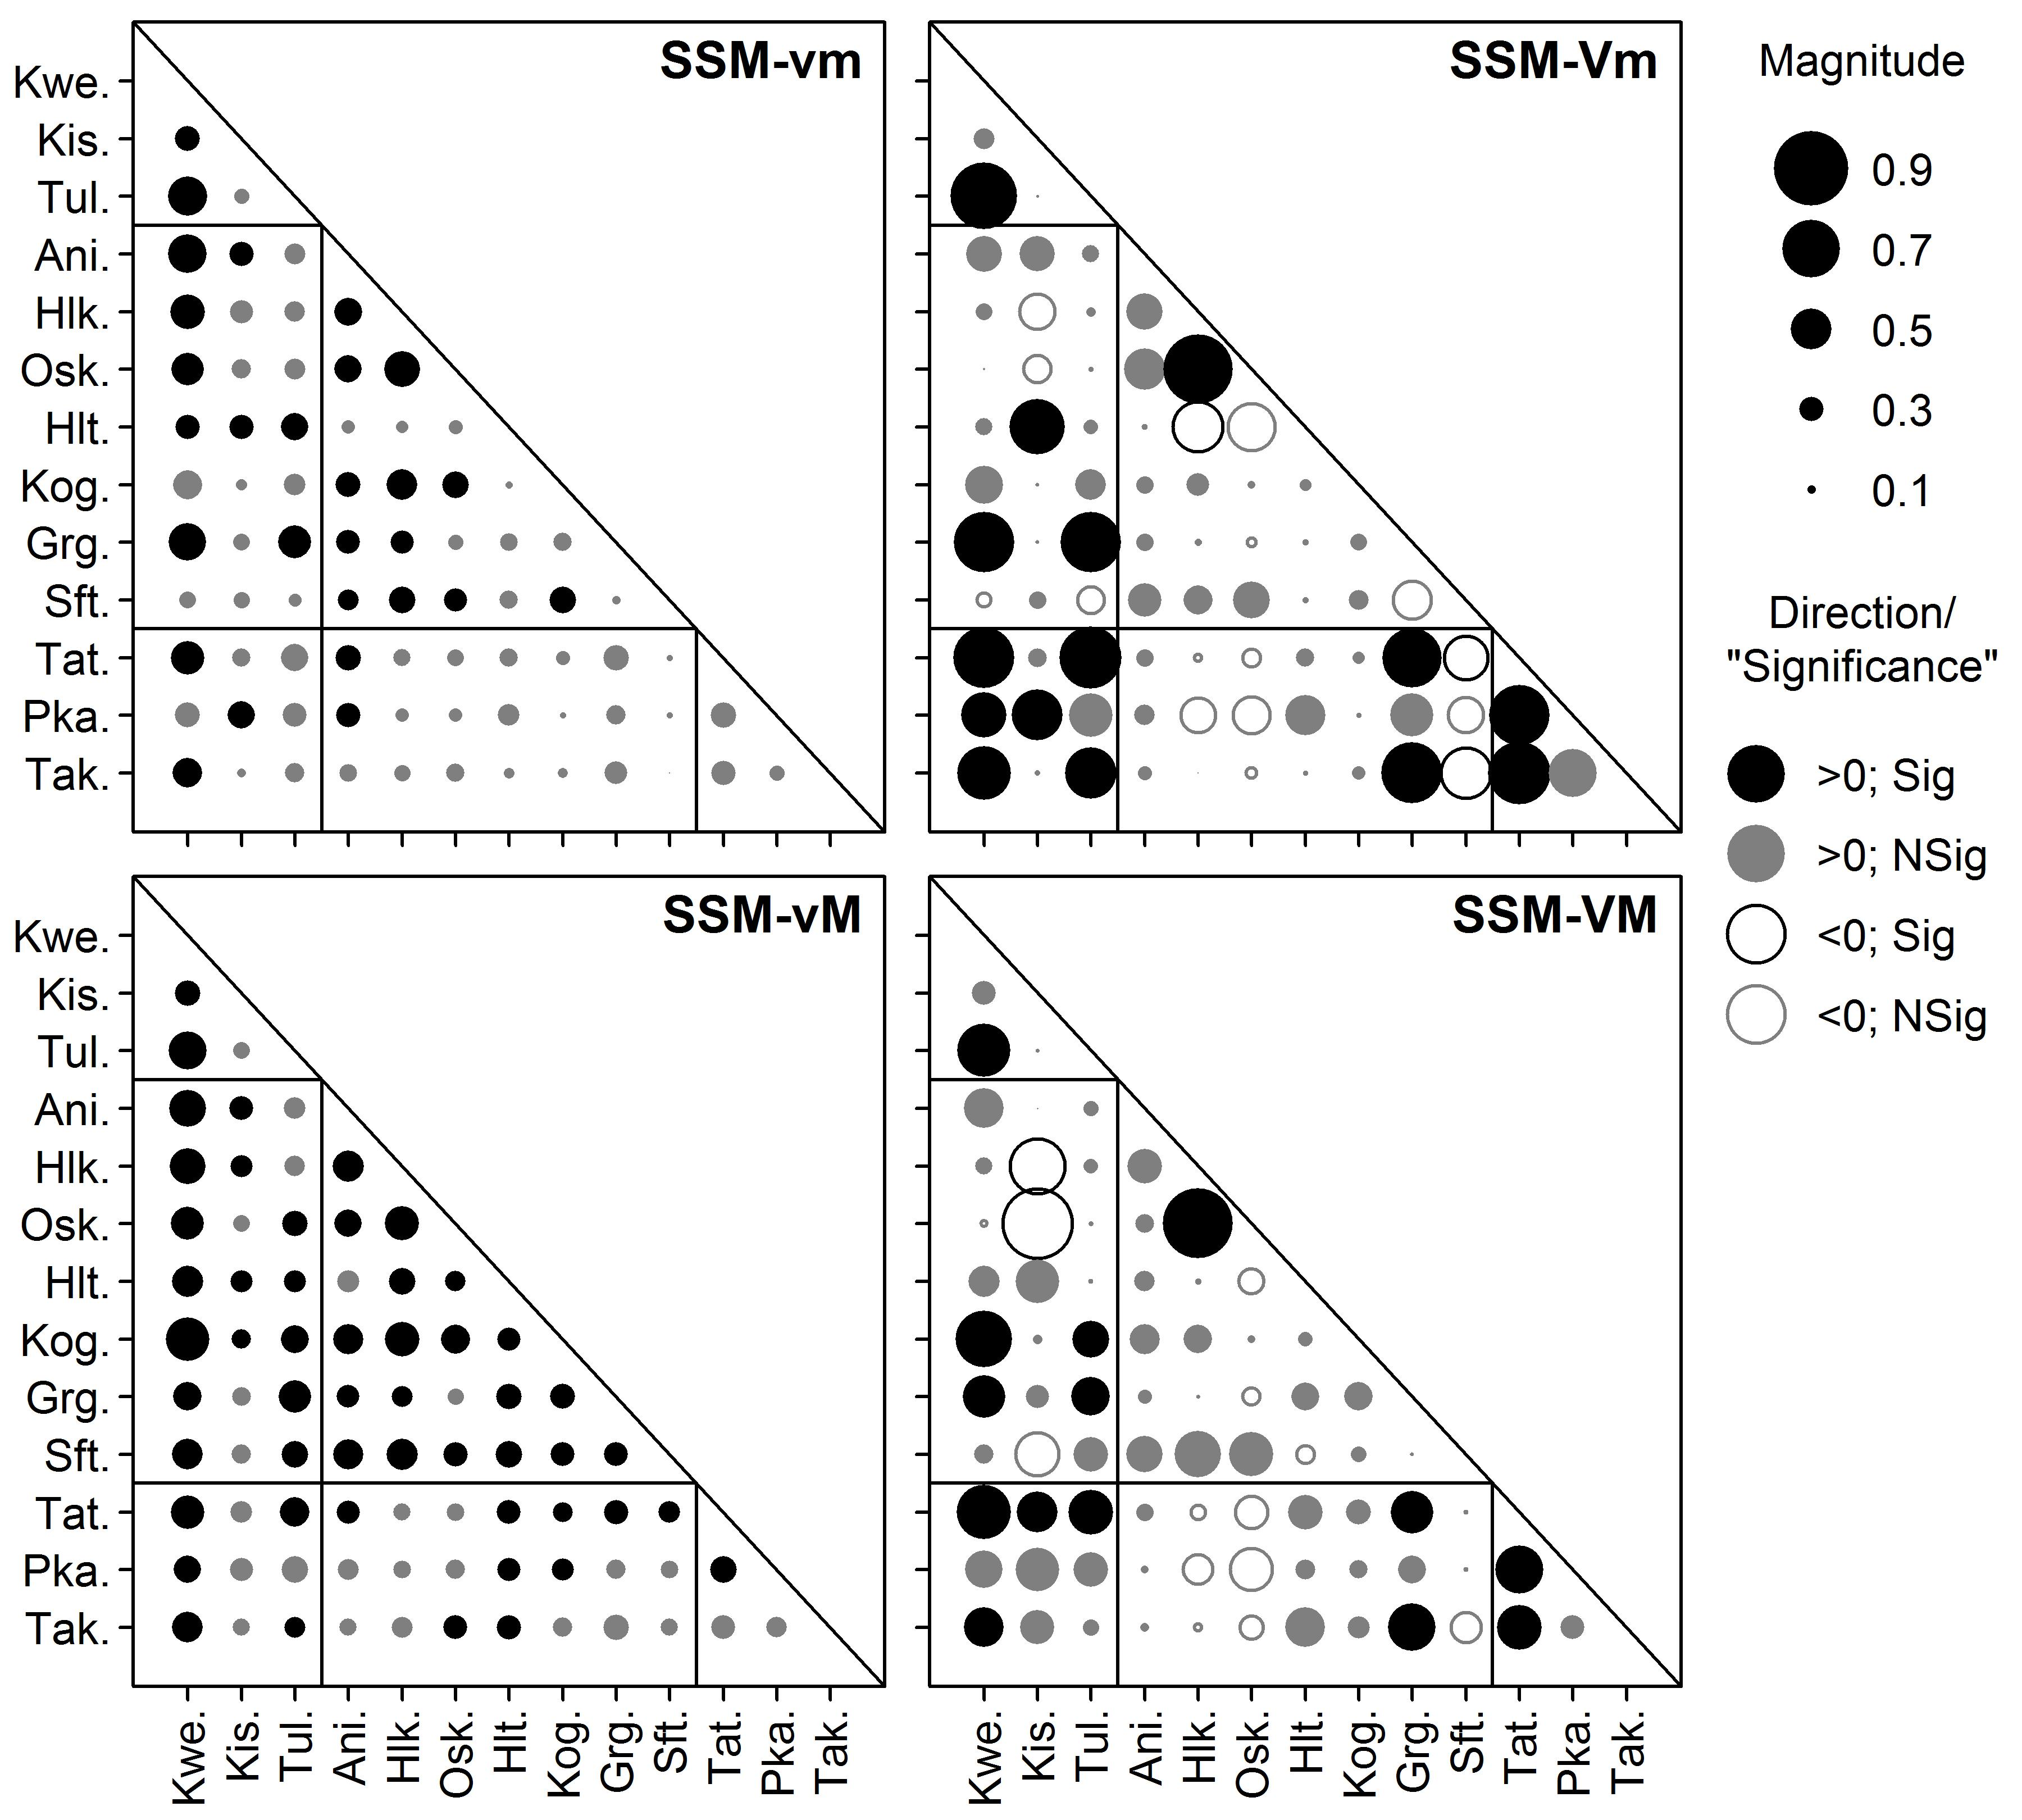
\includegraphics{img/Ch4/rhos.jpg}
  \caption{Correlation coefficients between recruitment residuals for each substock-pair. The size of each circle represents the magnitude of the correlation, color represents signficance (whether 95\% credible interval includes 0), and fill represents directionality as described in the legend. Substocks are ordered from downriver to upriver on both axes, and vertical/horizontal lines denote the boundaries between lower, middle, and upper river substocks.}
  \label{fig:rhos}
\end{figure}

\clearpage

\begin{figure}
  \centering
  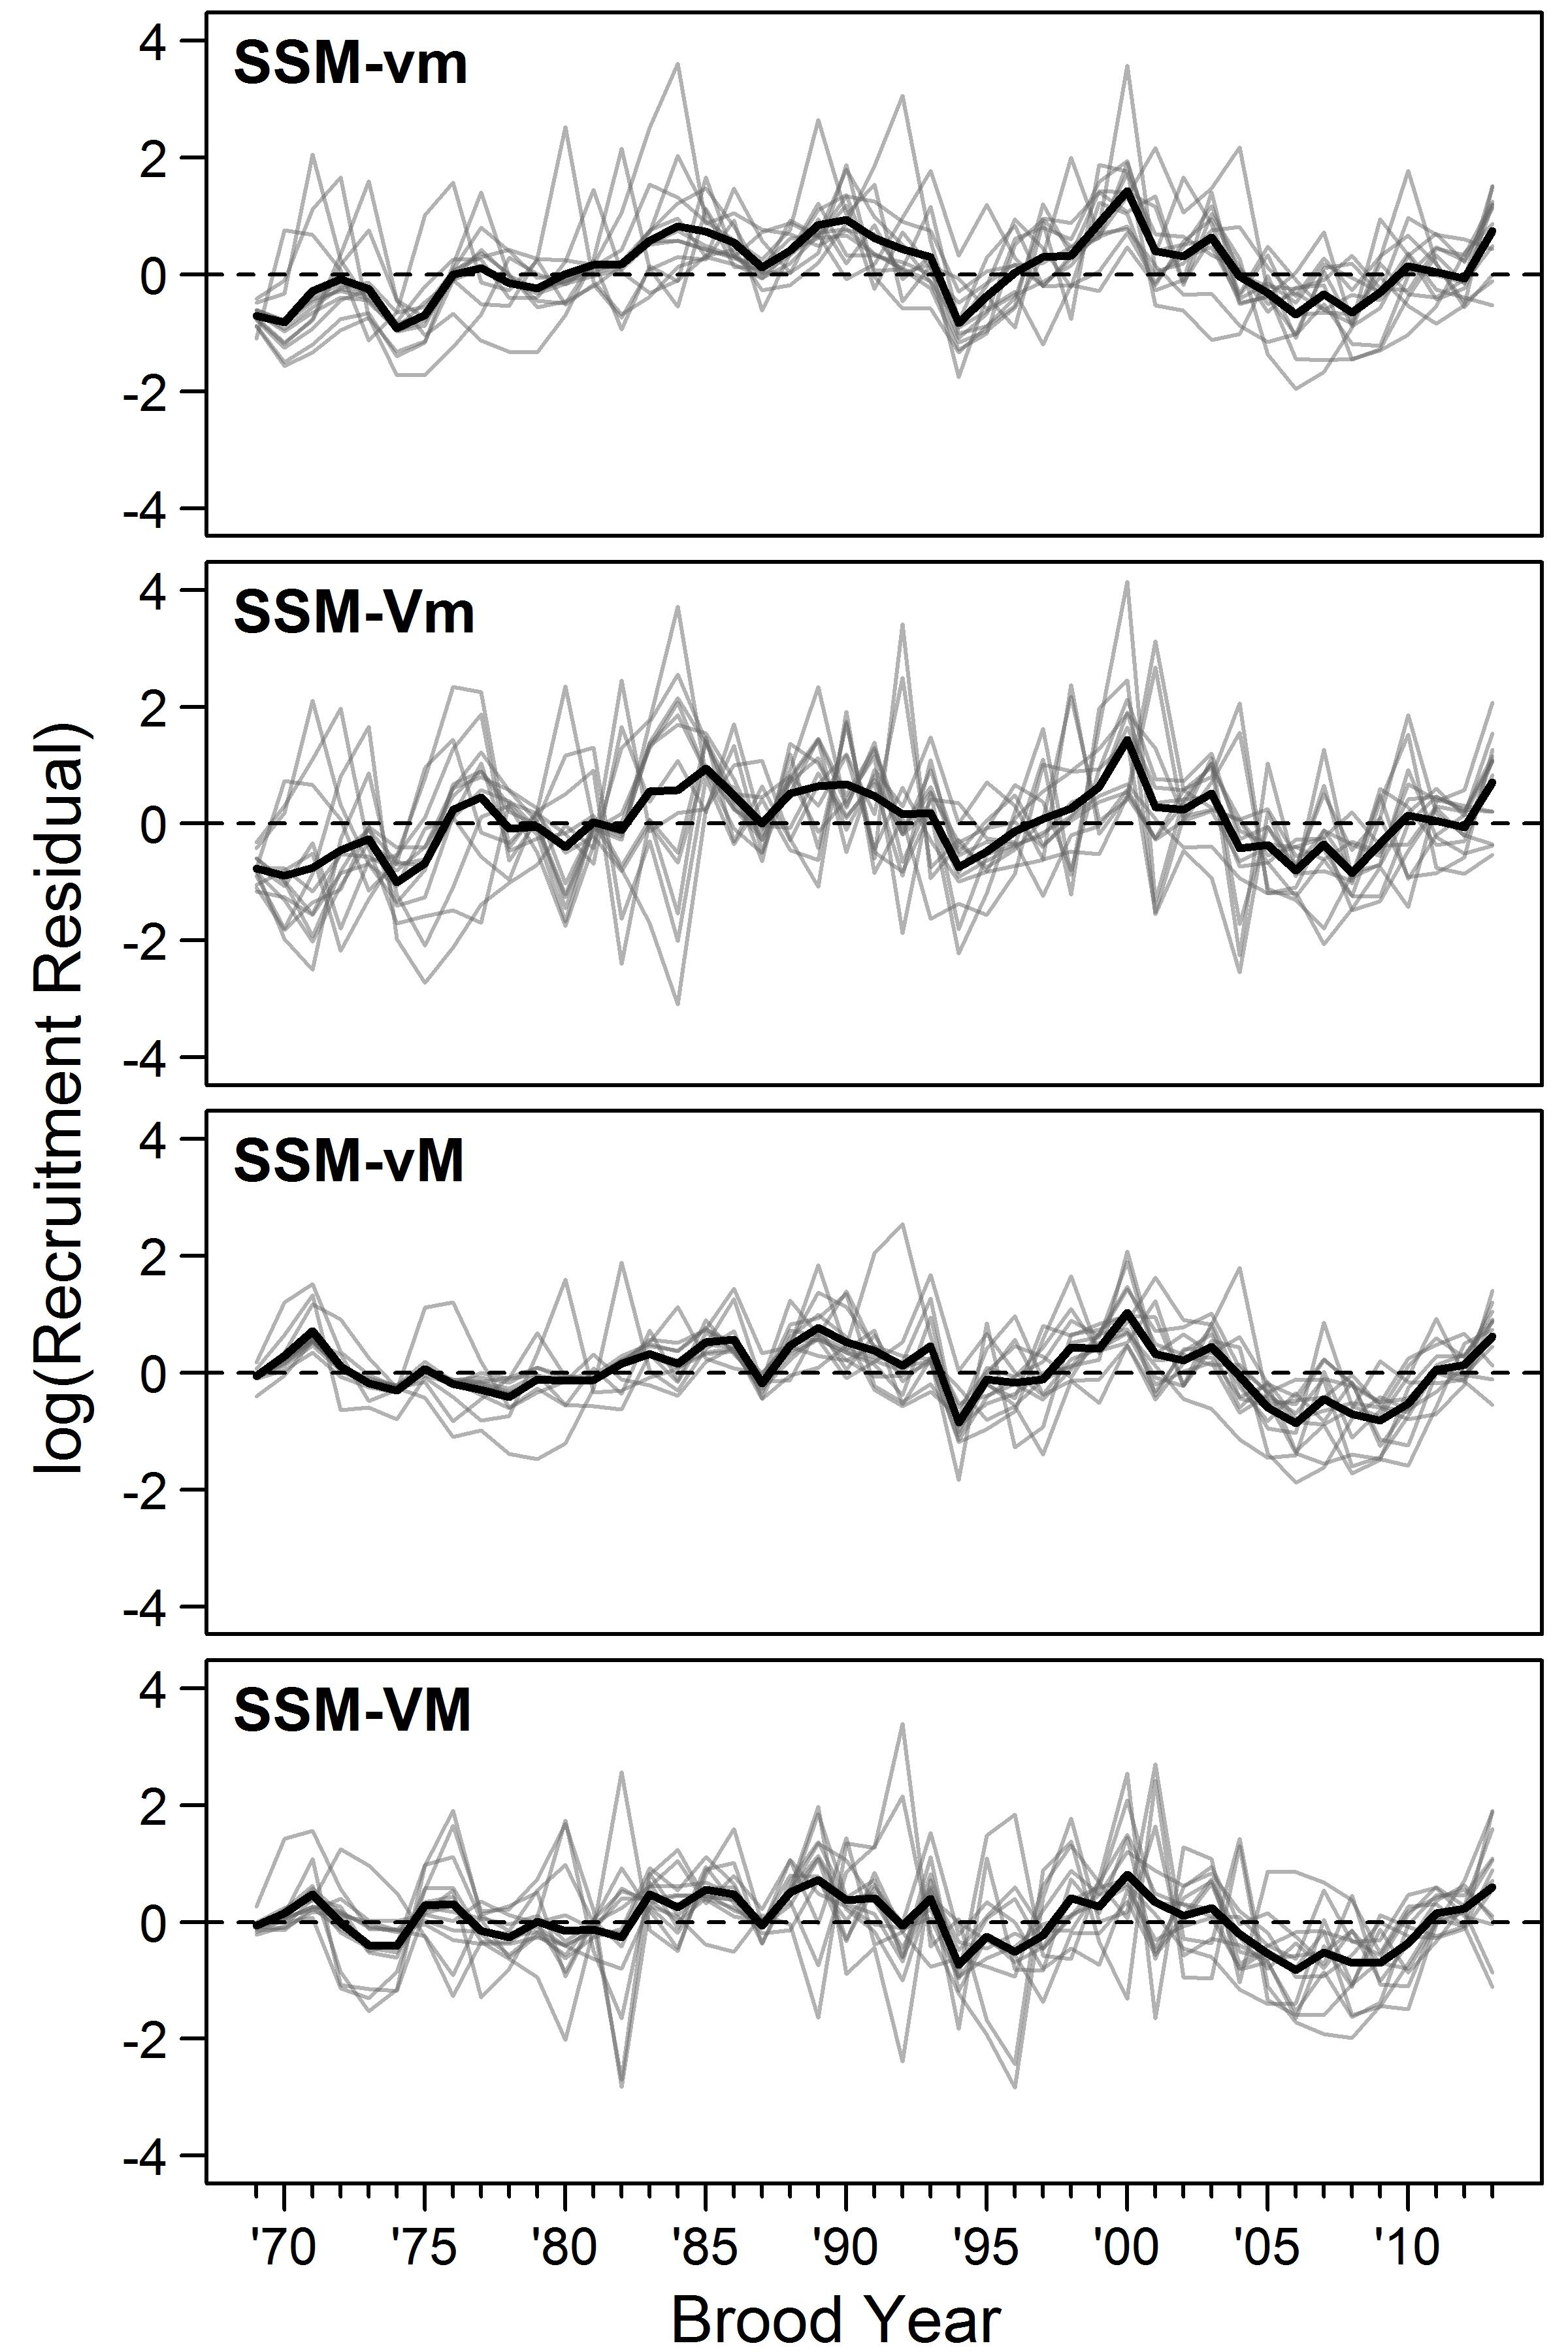
\includegraphics{img/Ch4/log-resids.jpg}
  \caption{Time series of recruitment residuals for each substock under each of the four state-space models. Substock-specific time series are represented by grey lines and the average across substocks within a brood year are represented by the thick black line. A dashed line at zero (no error) is provided for reference.}
  \label{fig:log-resids}
\end{figure}

\clearpage

\begin{figure}
  \centering
  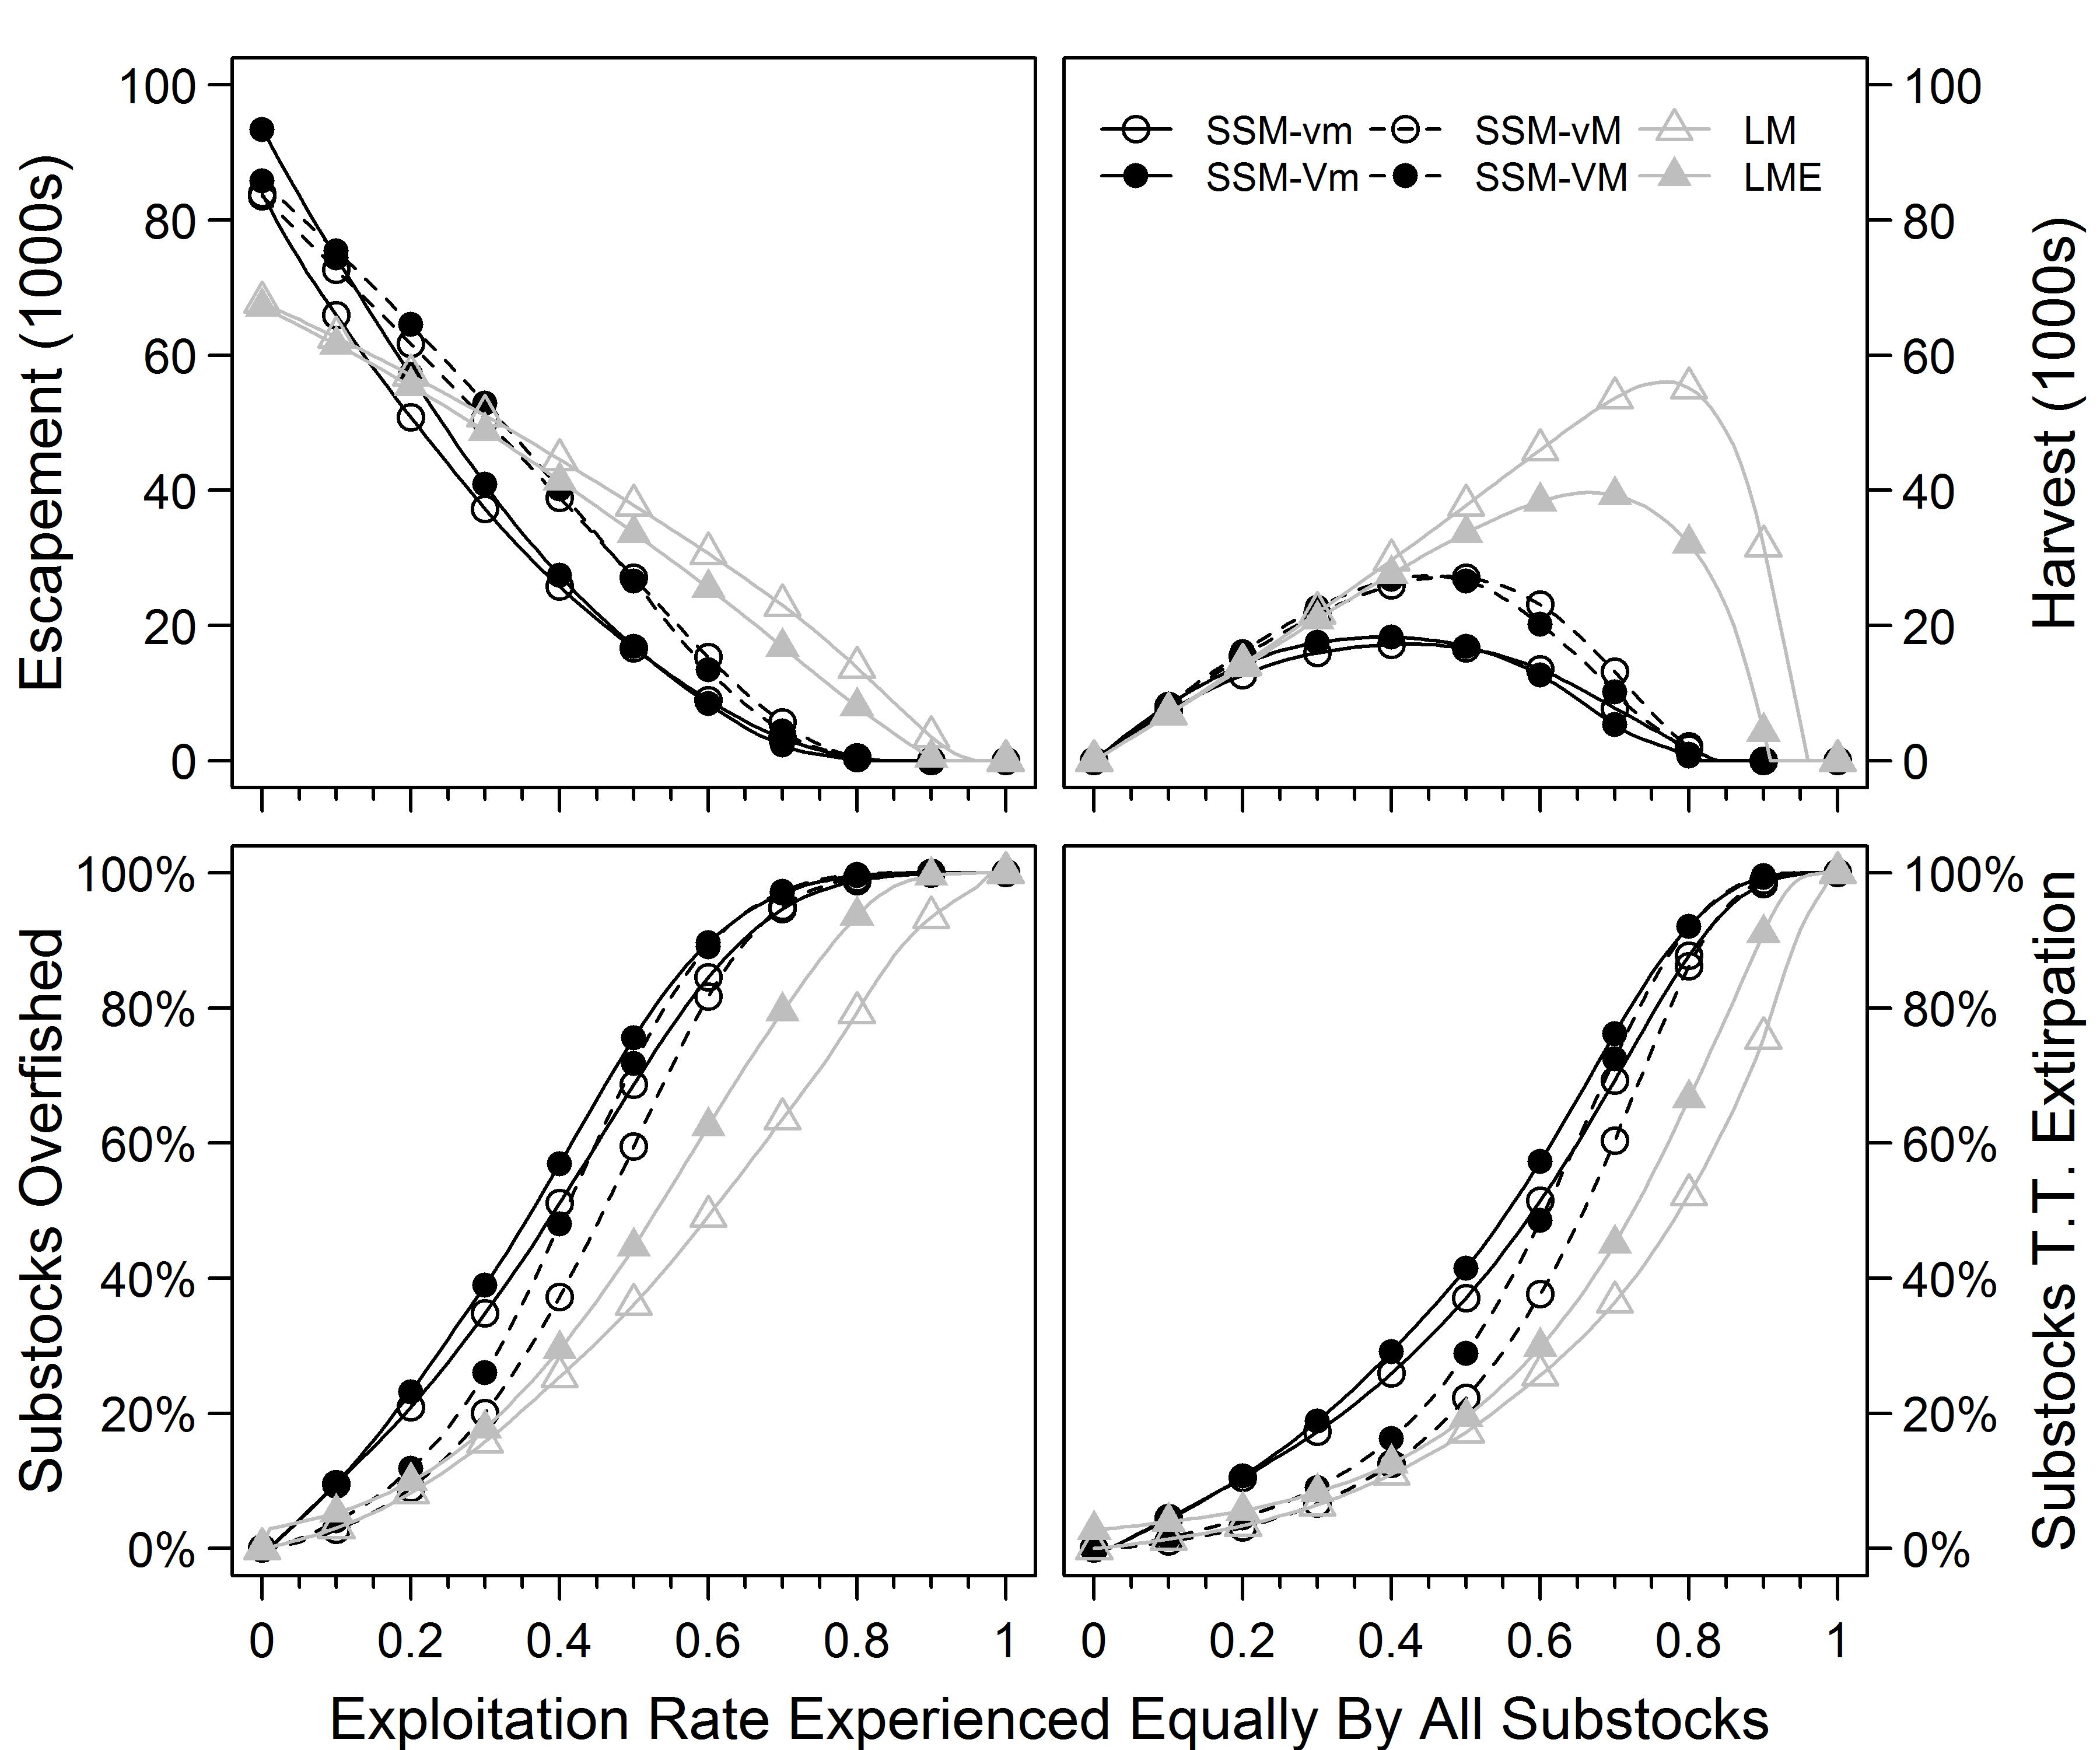
\includegraphics{img/Ch4/kusko-eq-states.jpg}
  \caption{Visualization of harvest-biodiversity trade-offs based on equilibrium states (escapement and harvest) of the aggregate stock and the percentage of substocks expected to be in an undesirable state as a function of the exploitation rate under the assumption that all substocks are fished at the same rate. Overfished is defined here as $U > U_{\text{MSY},j}$. ``T.T.'' stands for ``trending toward'', and represents the case where equilibrium escapement would be $\le 0$. To faciliate comparisons with the regression approaches (grey lines/triangles), the 3 substocks with insufficient data for fitting regression models were excluded from summaries of the state-space models (black triangles/circles).} 
  \label{fig:kusko-eq-states}
\end{figure}

\clearpage
\pagestyle{empty}

\begin{figure}
  \centering
  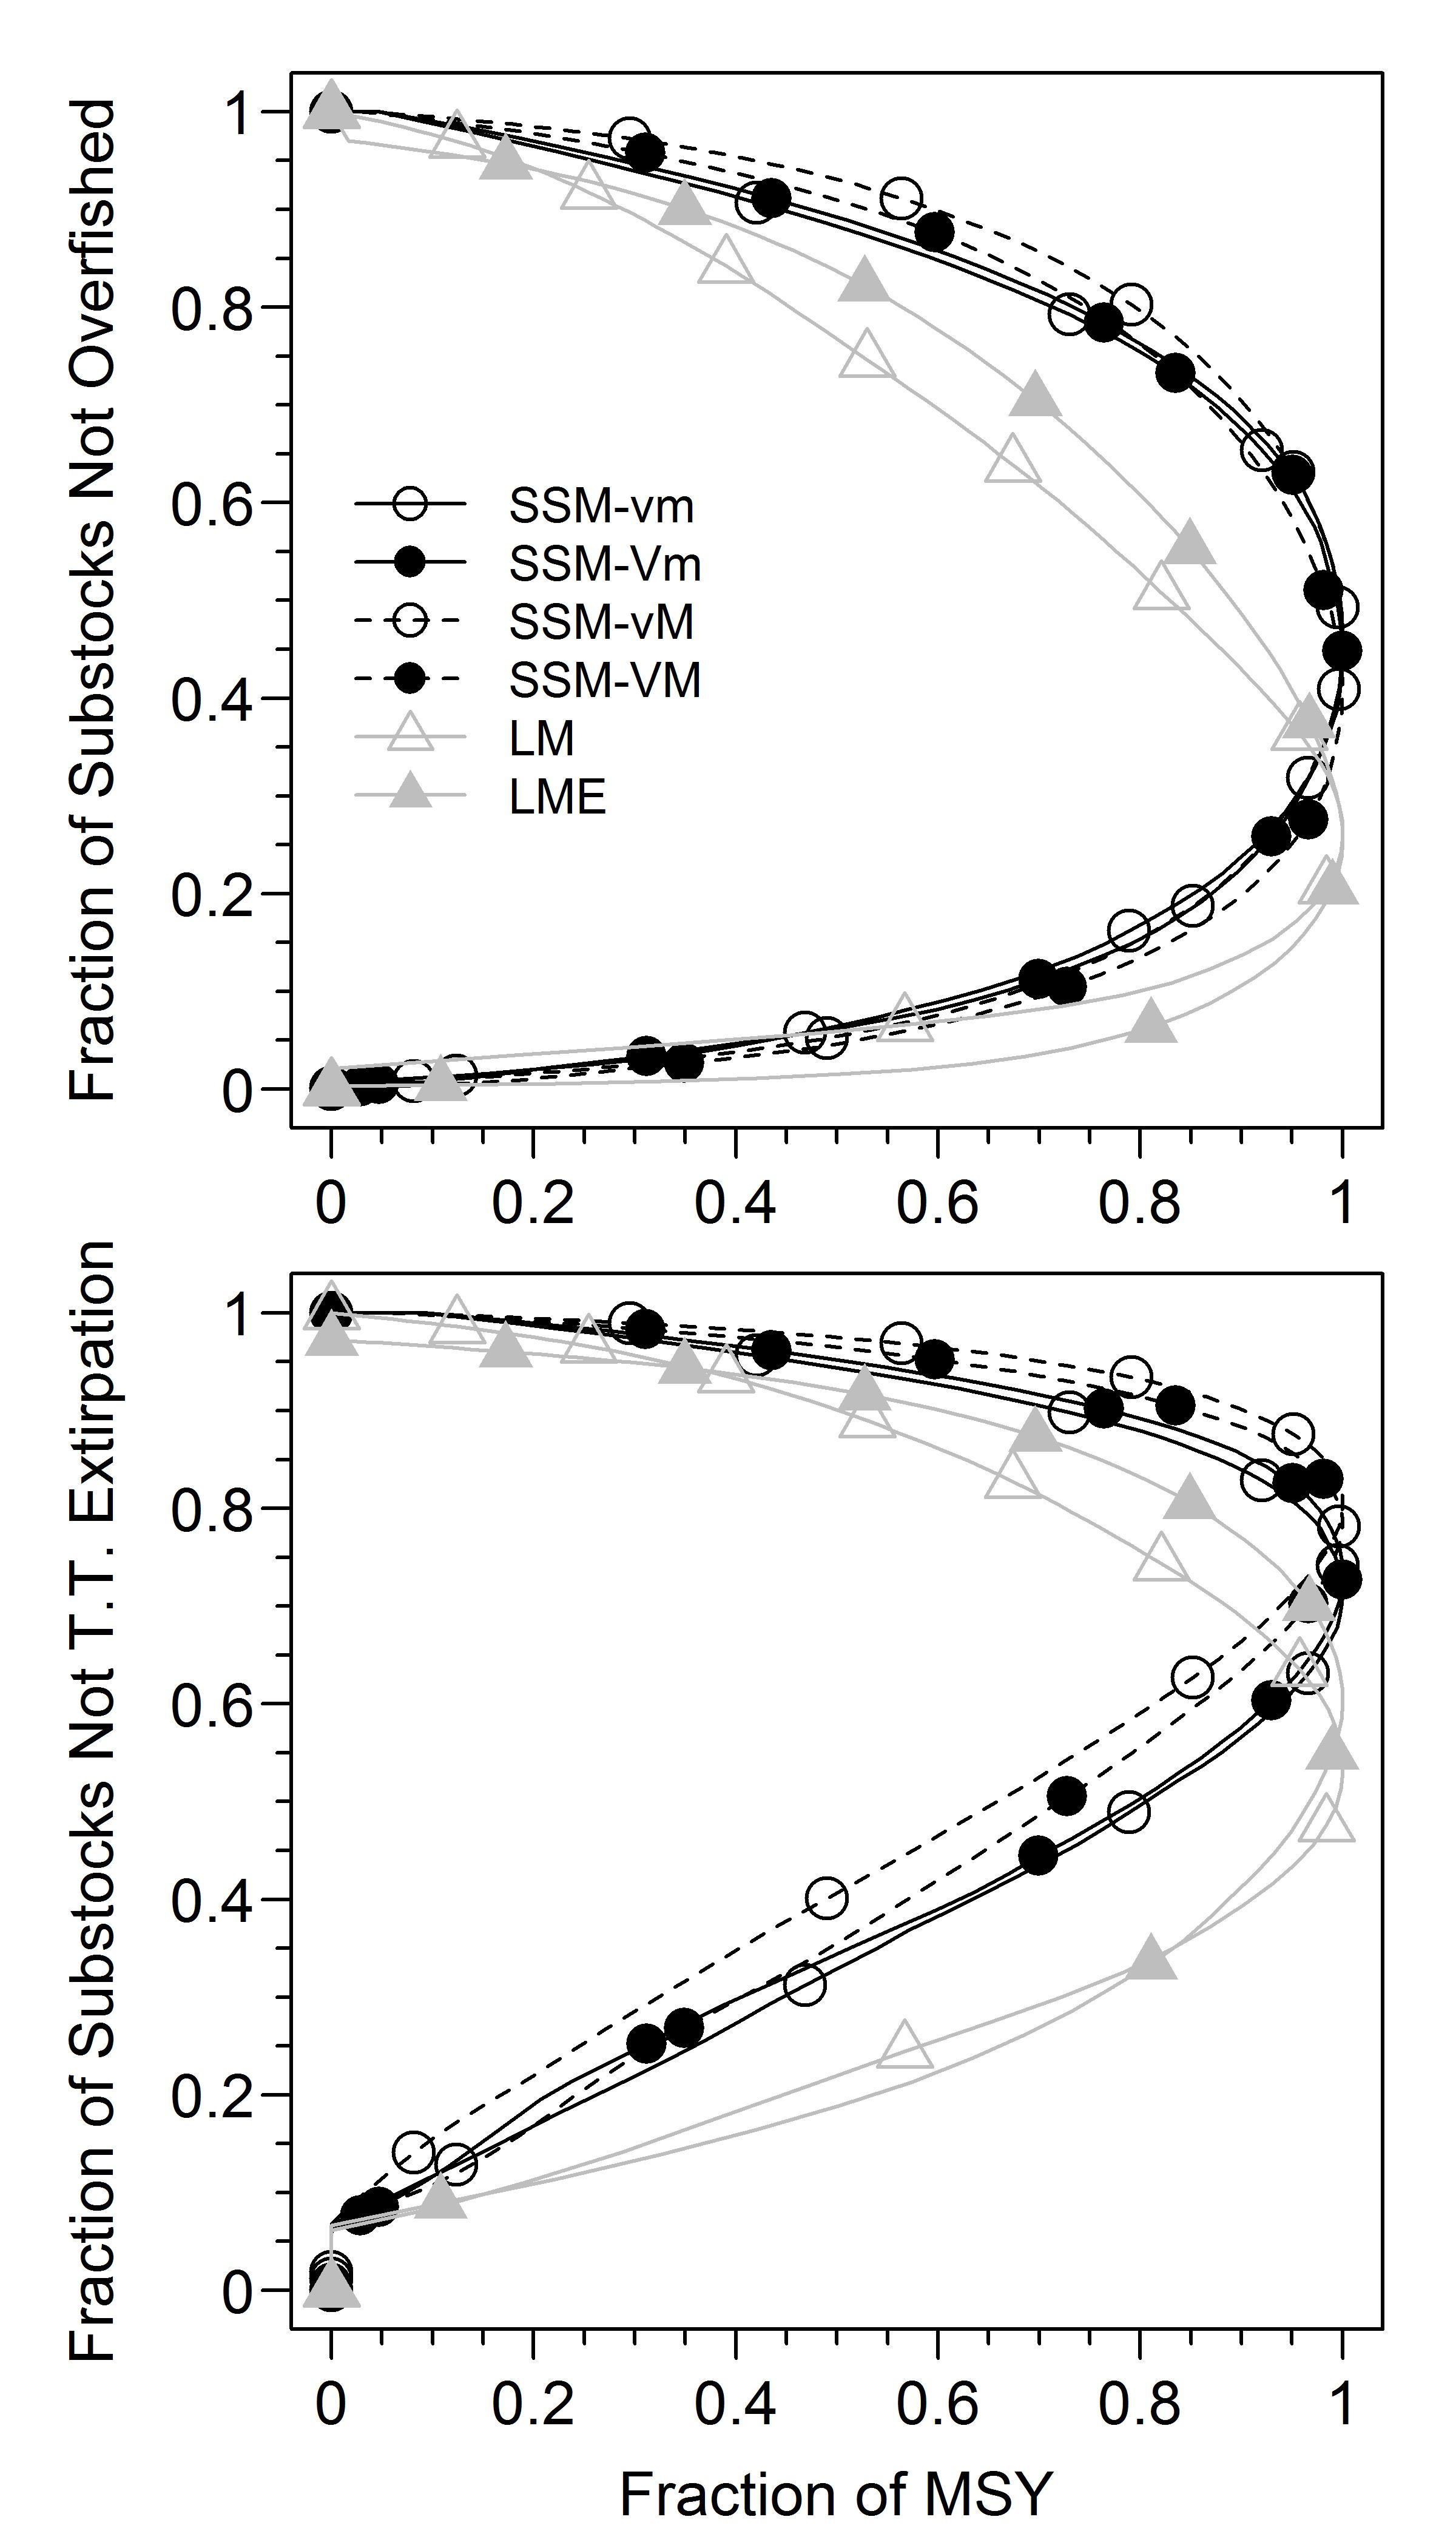
\includegraphics{img/Ch4/kusko-trade-offs.jpg}
  \caption{Alternate (and more direct than Figure \ref{fig:kusko-eq-states}) visualization of harvest-biodiversity trade-offs for monitored Kuskokwim River Chinook salmon substocks. The conditions of overfished and trending towards extinction are the same as defined in Figure \ref{fig:kusko-eq-states}. These figures should be interpreted by determining how the value of the biodiversity objective (\textit{y}-axis; expressed as the fraction of substocks that would not be in the undesirable condition) must be reduced to increase the value of the harvest objective (\textit{y}-axis; expressed as a fraction of the maximum sustainable yield). To faciliate comparisons with the regression approaches (grey lines/triangles), the 3 substocks with insufficient data for fitting regression models were excluded from summaries of the state-space models (black triangles/circles). All symbols represent increasing exploitation rates in increments of 0.1 as you move down the \textit{y}-axis.}
  \label{fig:kusko-trade-offs}
\end{figure}

\clearpage
\pagestyle{plain}

\doublespacing

\setlength{\parskip}{6pt plus 2pt minus 1pt}

\appendix


\captionsetup[figure]{list=yes} \captionsetup[table]{list=yes}

\chapter{Preparation of Data for Fitting Spawner-Recruit Models to
Substocks of Kuskokwim River Chinook Salmon in Chapter
\ref{ch4}}\label{appendix-c}

\section{Overview of data needs}\label{overview-of-data-needs}

\noindent
All data for this analysis are available to the public, and came
primarily from the Arctic-Yukon-Kuskokwim Database Management System
(AYKDBMS)\footnote{\url{http://www.adfg.alaska.gov/CommFishR3/WebSite/AYKDBMSWebsite/Default.aspx}}
maintained by the Alaska Department of Fish and Game (ADF\&G). Cases in
which other data sources were necessary are highlighted in the
description below, e.g., the telemetry data needed to perform the
expansion of aerial survey counts described in Section
\ref{air-expansion} below.

\noindent
This analysis required three primary data sources:

\begin{enumerate}
\def\labelenumi{(\arabic{enumi})}
\item
  Estimates of annual escapement to each of the substocks included.
\item
  Estimates of annual harvest. Linear regression models (Section
  \ref{reg-methods}) required harvest apportioned to each substock, the
  state-space models (Section \ref{ssm-model}) required only total
  aggregate harvest summed across all substocks included.
\item
  Estimates of annual age composition (i.e., the fraction of the run
  each year made up of each age) for all substocks that have had it
  collected.
\end{enumerate}

\noindent
Any of these data sources could have missing years.

\section{Substock escapement}\label{air-expansion}

\noindent
Escapement count data for this analysis were informed predominately by
the ADF\&G Kuskokwim River salmon escapement monitoring program, the
details of which have been most-recently documented in
\citet{head-liller-2017}. The data set available spans 20 different
escapement monitoring projects (6 weirs and 14 aerial surveys) and 42
calendar years from 1976 -- 2017. For substocks monitored \emph{via}
weir, observed substock \(j\) escapement in year \(t\) (\(S_{obs,t,j}\))
was taken to be the total estimated weir passage each year. Substocks
monitored \emph{via} aerial survey needed special care, however. Surveys
have been flown only once per year on a relatively small fraction of
each tributary system \citep{head-liller-2017}, resulting in these data
being indices of escapement rather than estimates of total escapement.
This analysis required estimates of total escapement to each substock
however, because this would allow calculation of biological reference
points that are expressed in terms of the scale of the population (e.g.,
the spawner abundance that is expected to produce maximum recruitment;
\(S_{\text{MAX},j}\)), rather than as a rate (i.e.,
\(U_{\text{MSY},j}\)). Note that if only estimates of
\(U_{\text{MSY},j}\) were desired, no accounting for the partial counts
would be necessary.

The approach I developed to estimate total escapement from single-pass
aerial surveys involved two main steps:

\begin{enumerate}
\def\labelenumi{(\arabic{enumi})}
\item
  Mapping the distribution of detected telemetry-tagged Chinook salmon
  against distribution of the aerial survey counts. This comparison
  allowed for a spatial expansion to estimate how many salmon would have
  been counted had the entire tributary been flown.
\item
  Obtaining and applying a temporal correction factor for the problem of
  counting a dynamic pool at one point in its trajectory. This
  correction factor was based on the relationship between paired weir
  and aerial counts on \(n=3\) of the systems in the analysis.
\end{enumerate}

\subsection{Spatial expansion}\label{spat-expansion}

\noindent
The core of the the spatial expansion estimator was the assumption:

\begin{equation}
  \frac{A_{f,t,i}}{T_{f,t,i}} = \frac{A_{u,t,i}}{T_{u,t,i}},
  \label{eq:air-expand1}
\end{equation}

\noindent
where the quantities \(A\) and \(T\) represent fish and tags,
respectively in flown (\(A_f\) and \(T_f\)) and unflown (\(A_u\) and
\(T_u\)) reaches in year \(t\) and for aerial survey monitoring project
\(i\). This assumption states that the ratio of spawners per one tagged
spawner is the same between flown and unflown river sections at the time
of the aerial index count and the aerial telemetry flights. Equation
\eqref{eq:air-expand1} and can be rearranged as:

\begin{equation}
  A_{u,t,i} = A_{f,t,i} \frac{T_{u,t,j}}{T_{f,t,i}}.
  \label{eq:air-expand2}
\end{equation}

\noindent
If \(T_{u,t,i}\) is further assumed to be a binomial random variable
with time-constant success parameter \(p_i\), then:

\begin{equation}
  T_{u,t,i} \sim \text{Binomial}(p_i,T_{u,t,i} + T_{f,t,i}).
  \label{eq:air-expand-binomial}
\end{equation}

\noindent
Here, \(p_i\) represents the probability that a tagged fish in the
spawning tributary monitored by project \(i\) was outside of the survey
flight reach at the time of the aerial telemetry flight. When
\eqref{eq:air-expand-binomial} is rearranged to put \(p_i\) on the odds
scale, then:

\begin{equation}
  \psi_i=\frac{p_i}{1-p_i}.
  \label{eq:air-expand-odds}
\end{equation}

\noindent
Estimated expansion factors \(\psi_i\) and \(p_i\) are shown in Table
\ref{tab:spat-expand-table}. The odds value \(\psi_i\) can be
substitiuted for the division term in \eqref{eq:air-expand2} which gives:

\begin{equation}
  A_{u,t,i} = A_{f,t,i} \psi_i.
  \label{eq:air-expand3}
\end{equation}

\noindent
To obtain the total number of fish that would have been counted had the
entire subdrainage been flown (\(\hat{A}_{t,i}\)), the components can be
summed:

\begin{equation}
  \hat{A}_{t,i} = A_{f,t,i} + A_{u,t,i}.
  \label{eq:air-expand4}
\end{equation}

\noindent
Substistituion of \eqref{eq:air-expand3} into \eqref{eq:air-expand4} and
factoring gives the estimator:

\begin{equation}
  \hat{A}_{t,i}=A_{f,t,i}(1 + \psi_i).
  \label{eq:air-expand-final}
\end{equation}

\noindent
The spatial expansion model was integrated with the temporal expansion
model described below into a single model fitted in the Bayesian
framework fitted using JAGS \citep{plummer-2017}. This allowed for
seamless propogation of uncertainty (in \(\psi_i\)) from the expansion
above to the next step.

\subsection{Temporal Expansion}\label{temp-expansion}

\noindent
The temporal expansion model was necessary to convert from the one-pass
index scale to the substock total annual escapement scale: it was a
temporal correction. The temporal expansion I developed operated by
first regressing \(n = 16\) observations of paired weir count (\(W_i\))
and spatially-expanded aerial counts (\(\hat{A}_{i}\); given by
\eqref{eq:air-expand-final}) on the same tributary systems (\(n = 3\)) in
the same years:

\begin{equation}
  \begin{split}
    W_i = \beta_0 + \beta_1 \hat{A}_i + \varepsilon_i, \\
    \varepsilon_i \stackrel{\text{iid}}{\sim} N(0, \sigma_W) \\
  \end{split}
\label{eq:temp-expand1}
\end{equation}

The estimated coefficients \(\hat{\beta}_0\) and \(\hat{\beta}_1\)
(Table \ref{tab:temp-expand-table}) were then applied to tributary
systems with an aerial count but not a weir count:

\begin{equation}
  S_{obs,t,j}=\hat{\beta}_0 + \hat{\beta}_1 \hat{A}_{t,j}
\label{eq:temp-expand2}
\end{equation}

\noindent
The fitted relationship is shown in Figure \ref{fig:obs-correct}. For
substocks that had both weirs and aerial surveys, the weir count was
used as \(S_{obs,t,j}\) as opposed to using the expansion in
\eqref{eq:temp-expand2} and the coefficient of variation (CV) representing
observation uncertainty for the state-space models (Section
\ref{ssm-obs-model}) was set at 5\%, which assumed annual escapement
counts made at weirs are precise. For substocks monitored solely
\emph{via} aerial survey, the posterior mean value of \(S_{obs,t,j}\)
was used as the escapement count that year, and the posterior CV was
calculated for use as the observation uncertainty passed to the
state-space models.

\section{Aggregate harvest}\label{harv-expansion}

\noindent
Harvest estimates for the Kuskokwim River are available at the
drainage-wide scale only, and were obtained each year by subtracting the
drainage-wide estimates of total run and escapement
\citep{liller-etal-2018}. Because the escapement data used here do not
encompass all the substocks within the Kuskokwim River system, it was
necessary to remove some portion of the total harvest that was produced
by stocks not included in this analysis. First, I calculated the
observed exploitation rate of the drainage-wide Kuskokwim River Chinook
salmon stock (\(U_{obs,t}\)) by dividing the total harvest by the total
run each year. I then made the assumption that monitored and unmonitored
substocks have received the same exploitation rates, in which case total
harvest accounted for in this analysis harvest was be obtained as:

\begin{equation}
  H_{obs,t} = \frac{S_{obs,t} U_{obs,t}}{1-U_{obs,t}},
  \label{eq:H-obs}
\end{equation}

\noindent
which can be derived from the definition of the exploitation rate
\(\left(U = \frac{H}{S+H}\right)\). This step was embedded within the
same Bayesian model that encompassed the spatial and temporal aerial
survey expansions such that uncertainty in these steps could be
propagated through the entire analysis. The posterior mean value of
\(H_{obs,t}\) was used as the observed total harvest data, and the
posterior CV was retained for use as the observation error attributed to
this data source.

Note that \(S_{obs,t}\) and \(H_{obs,t}\) do not have \(j\) subscripts
denoting particular substocks: this indicates that they are aggregate
quantities summed across all substock components. In cases where
substock-specific harvest was desired (i.e., in reconstructing the
substock-specific brood tables for fitting individual regression
relationships; Section \ref{lm-btable}), \(H_{obs,t,j}\) was obtained
using \eqref{eq:H-obs} by substituting \(S_{obs,t,j}\) in for
\(S_{obs,t}\).

\section{Age composition}\label{age-comp}

\noindent
Age composition data were necessary to reconstruct brood tables for
age-structured salmon populations (see Section \ref{lm-btable}). Age
data used in this analysis came from the ADF\&G standardized age, sex,
and length sampling program operated at the weir projects. All sampled
fish that were not aged successfully were discarded as were samples
corresponding to the rare ages of 3 and 8 such that only fish
successfully aged as between 4 and 7 were included. It is possible that
older or younger fish may have the systematic tendency to return early
or late in the run, and this could introduce biases if age sampling was
not conducted proportionally to fish passage throughout the season. To
adjust for this possibility, a weighted-average scheme was applied to
obtain the age composition estimates for each substock and year with
data. Daily age samples were stratified into two-week strata and
strata-specific proportions-at-age were calculated. These
strata-specific age compositions were then averaged across strata within
a year and stock weighted by the number of Chinook salmon estimated to
have passed the weir in each stratum. The total number of fish
successfully aged for each year and substock was retained for
data-weighting purposes for the state-space models (see Section
\ref{ssm-obs-model}).

\clearpage

\singlespacing

\begin{table}

\caption{\label{tab:spat-expand-table}The estimated spatial expansion factors for the various aerial survey projects described in Section \ref{spat-expansion}. $p_i$ represents the average fraction of telemetry tags that were detected outside of index flight reaches, which was used as the basis for determining the multiplier ($1 + \psi_i$) needed to correct the aerial count for not flying the entire subdrainage. In cases where multiple projects were flown to count fish within one substock (e.g., the Aniak, see Figure \ref{fig:ch4-map} substock 4), the expanded project counts were summed to obtain an estimate for the total substock, as indicated by the footnotes.}
\centering
\begin{tabular}[t]{lcclcclcc}
\toprule
\textbf{Aerial Survey} & $\boldsymbol{p_i}$ & $\boldsymbol{1 + \psi_i}$\\
\midrule
\textbf{Kisaralik} & \makecell[c]{0.59\\(0.42 -- 0.75)} & \makecell[c]{2.46\\(1.72 -- 4.04)}\\
\textbf{Salmon (Aniak)}\textsuperscript{a} & \makecell[c]{0.04\\(0.01 -- 0.12)} & \makecell[c]{1.04\\(1.01 -- 1.14)}\\
\textbf{Aniak}\textsuperscript{a} & \makecell[c]{0.41\\(0.37 -- 0.47)} & \makecell[c]{1.71\\(1.58 -- 1.87)}\\
\textbf{Kipchuk}\textsuperscript{a} & \makecell[c]{0.09\\(0.04 -- 0.17)} & \makecell[c]{1.1\\(1.04 -- 1.21)}\\
\textbf{Holokuk} & \makecell[c]{0.37\\(0.23 -- 0.53)} & \makecell[c]{1.59\\(1.3 -- 2.12)}\\
\textbf{Oskawalik} & \makecell[c]{0.44\\(0.29 -- 0.6)} & \makecell[c]{1.79\\(1.4 -- 2.52)}\\
\textbf{Holitna} & \makecell[c]{0.79\\(0.75 -- 0.83)} & \makecell[c]{4.78\\(4.04 -- 5.73)}\\
\textbf{Cheeneetnuk}\textsuperscript{b} & \makecell[c]{0.25\\(0.16 -- 0.38)} & \makecell[c]{1.34\\(1.18 -- 1.61)}\\
\textbf{Gagaryah}\textsuperscript{b} & \makecell[c]{0.08\\(0.02 -- 0.19)} & \makecell[c]{1.08\\(1.02 -- 1.24)}\\
\textbf{Salmon (Pitka Fork)}\textsuperscript{c} & \makecell[c]{0.4\\(0.3 -- 0.5)} & \makecell[c]{1.66\\(1.42 -- 2.01)}\\
\textbf{Bear}\textsuperscript{c} & \makecell[c]{0.05\\(0 -- 0.22)} & \makecell[c]{1.05\\(1 -- 1.28)}\\
\textbf{Upper Pitka Fork}\textsuperscript{c} & \makecell[c]{0.62\\(0.48 -- 0.75)} & \makecell[c]{2.62\\(1.92 -- 4)}\\
\bottomrule
\multicolumn{9}{l}{\textit{Substocks assessed with multiple aerial survey projects}}\\
\multicolumn{9}{l}{\textsuperscript{a} Aniak Substock}\\
\multicolumn{9}{l}{\textsuperscript{b} Swift Substock}\\
\multicolumn{9}{l}{\textsuperscript{c} Pitka Substock}\\
\end{tabular}
\end{table}

\clearpage

\begin{table}[H]

\caption{\label{tab:temp-expand-table}The estimated temporal expansion parameters for converting spatially-expanded aerial counts to estimates of subdrainage-wide escapement abundance each year.}
\centering
\begin{tabular}[t]{lcclcc}
\toprule
\textbf{Parameter} & \textbf{Estimate}\\
\midrule
$\hat{\beta_0}$ & \makecell[c]{1.9\\(-60.71 -- 62.4)}\\
$\hat{\beta_1}$ & \makecell[c]{2.3\\(1.76 -- 2.85)}\\
$\hat{\sigma_W}$ & \makecell[c]{4992.15\\(3376.54 -- 7565.08)}\\
\bottomrule
\end{tabular}
\end{table}

\clearpage

\begin{figure}
  \centering
  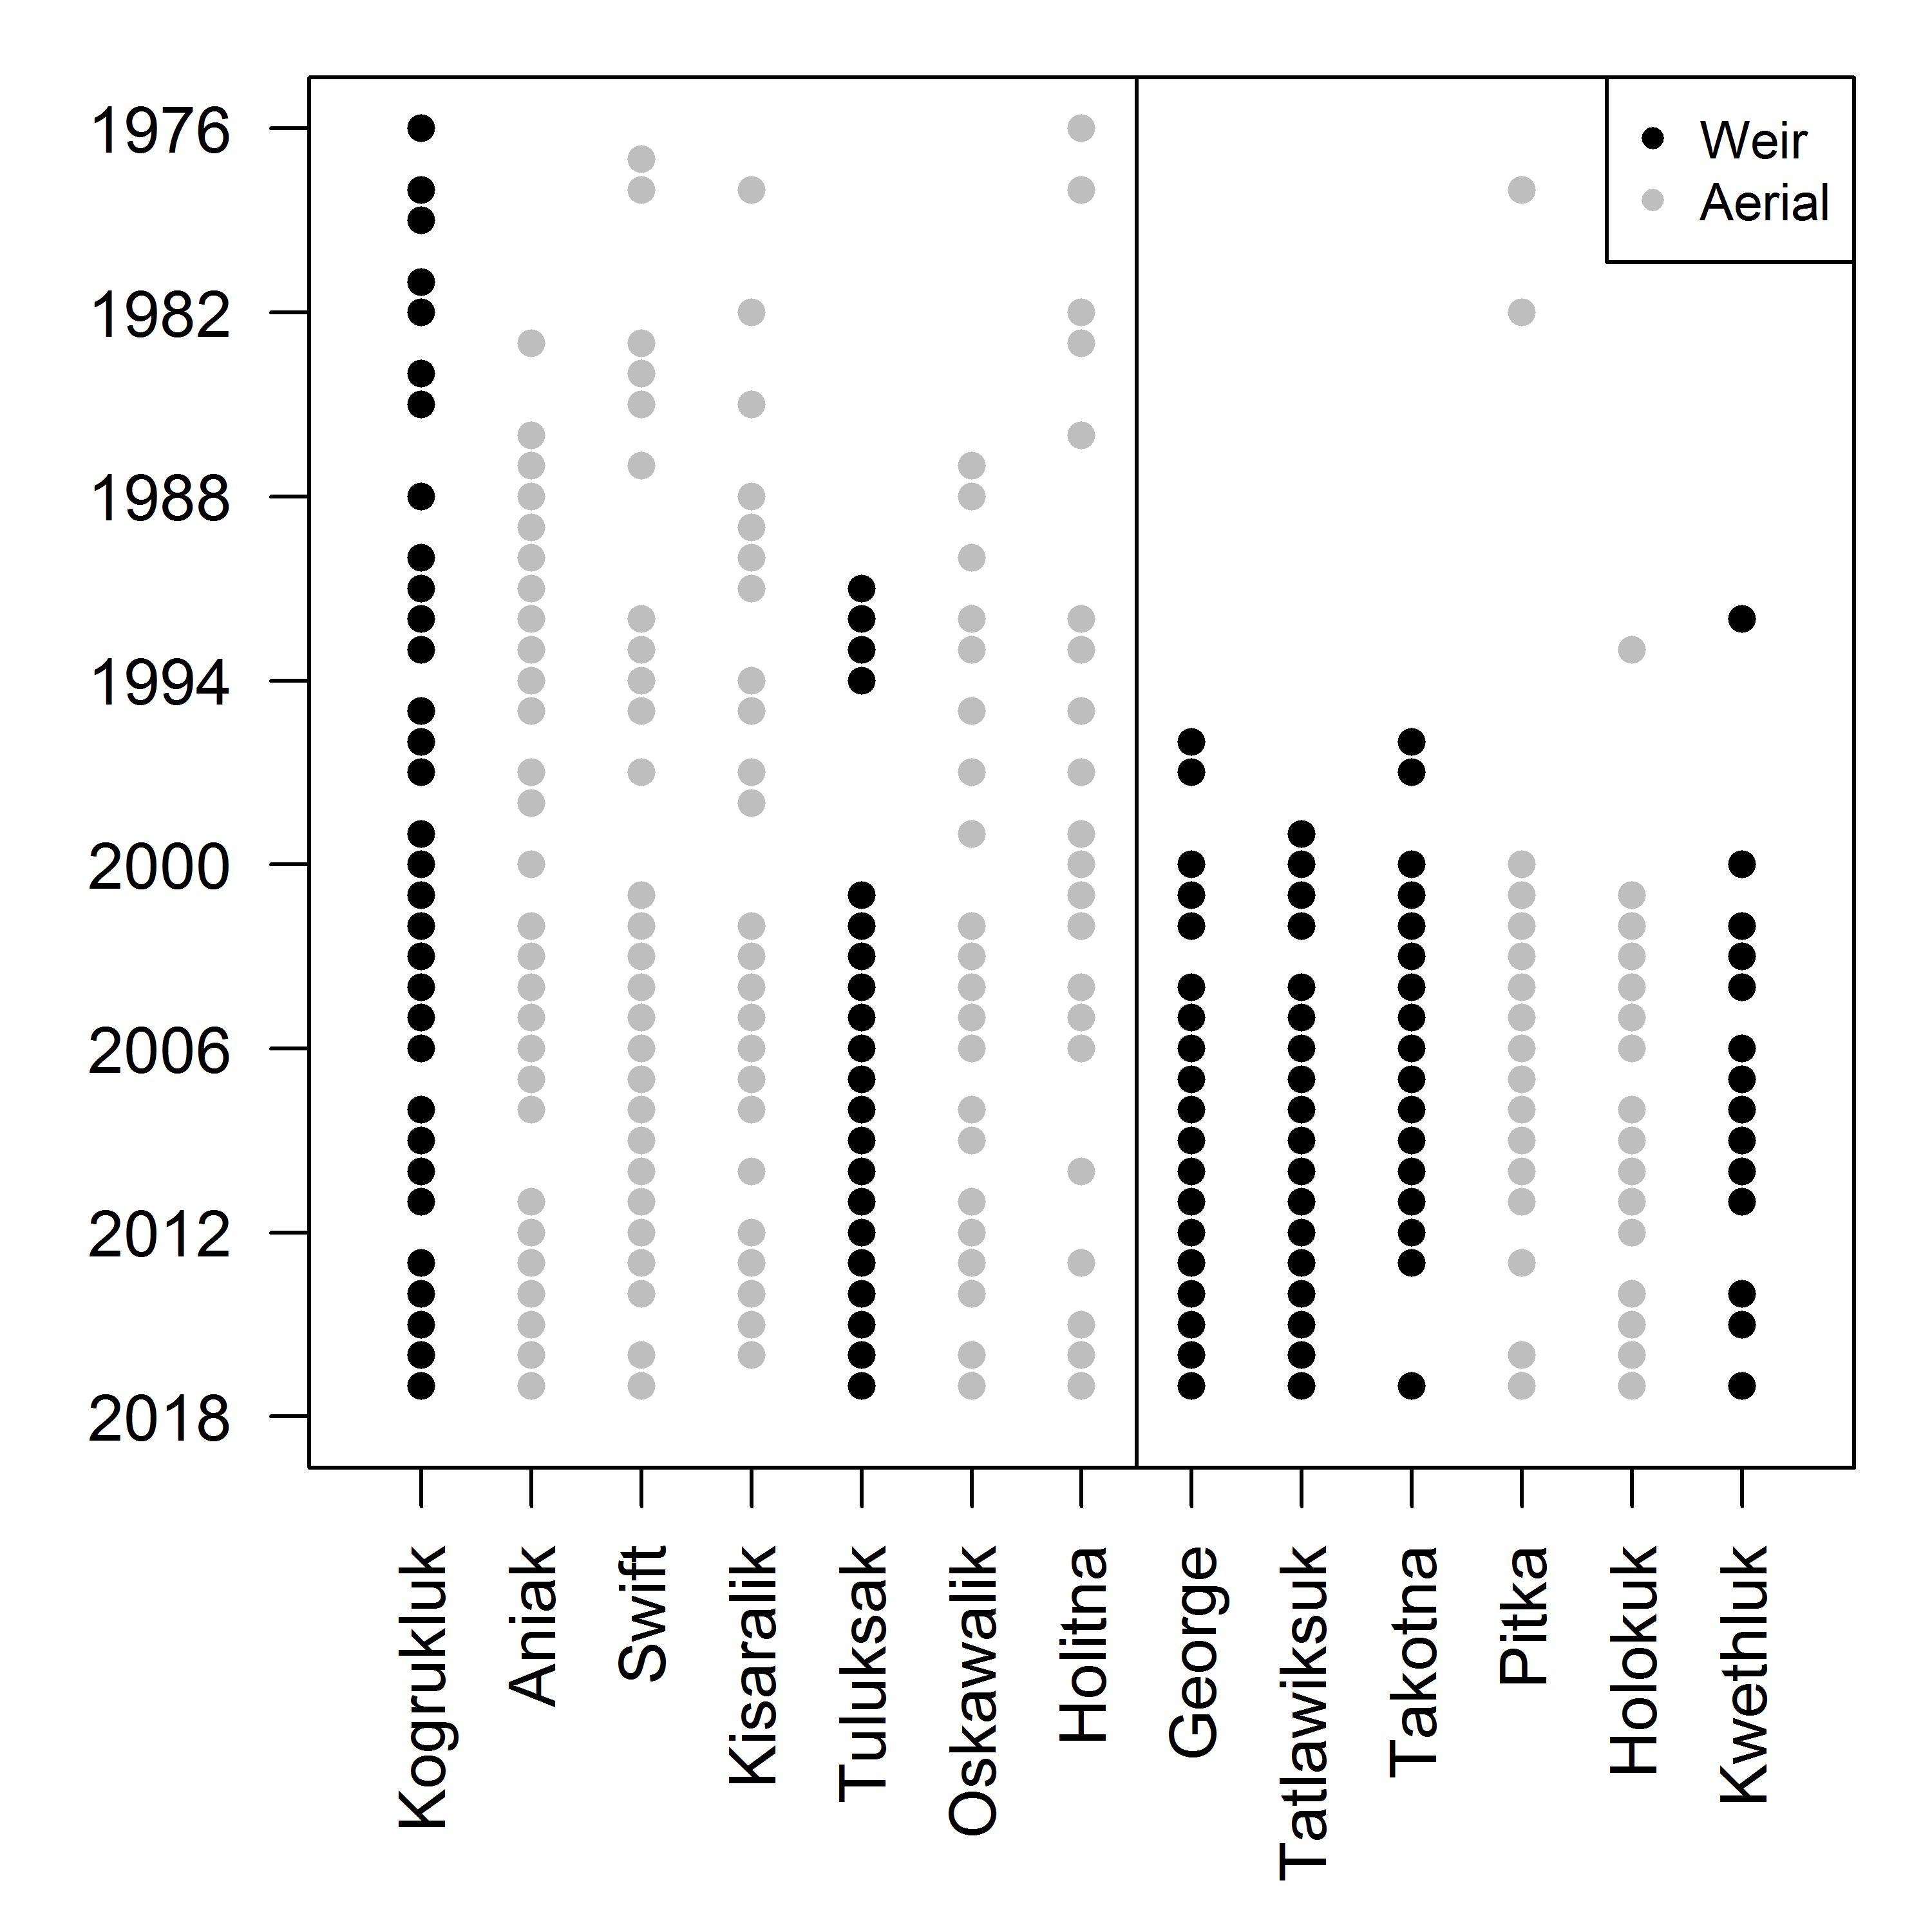
\includegraphics{img/Ch4/obs-freq.jpg}
  \caption{The frequency of escapement sampling for each substock sampled in the Kuskokwim River. Black points indicate years that were sampled for substocks monitored with a weir and grey points indicate years sampled for substocks monitored with aerial surveys. The vertical black line shows a break where > 50\% of the years were monitored for a stock.}
  \label{fig:obs-freq}
\end{figure}

\clearpage

\begin{figure}
  \centering
  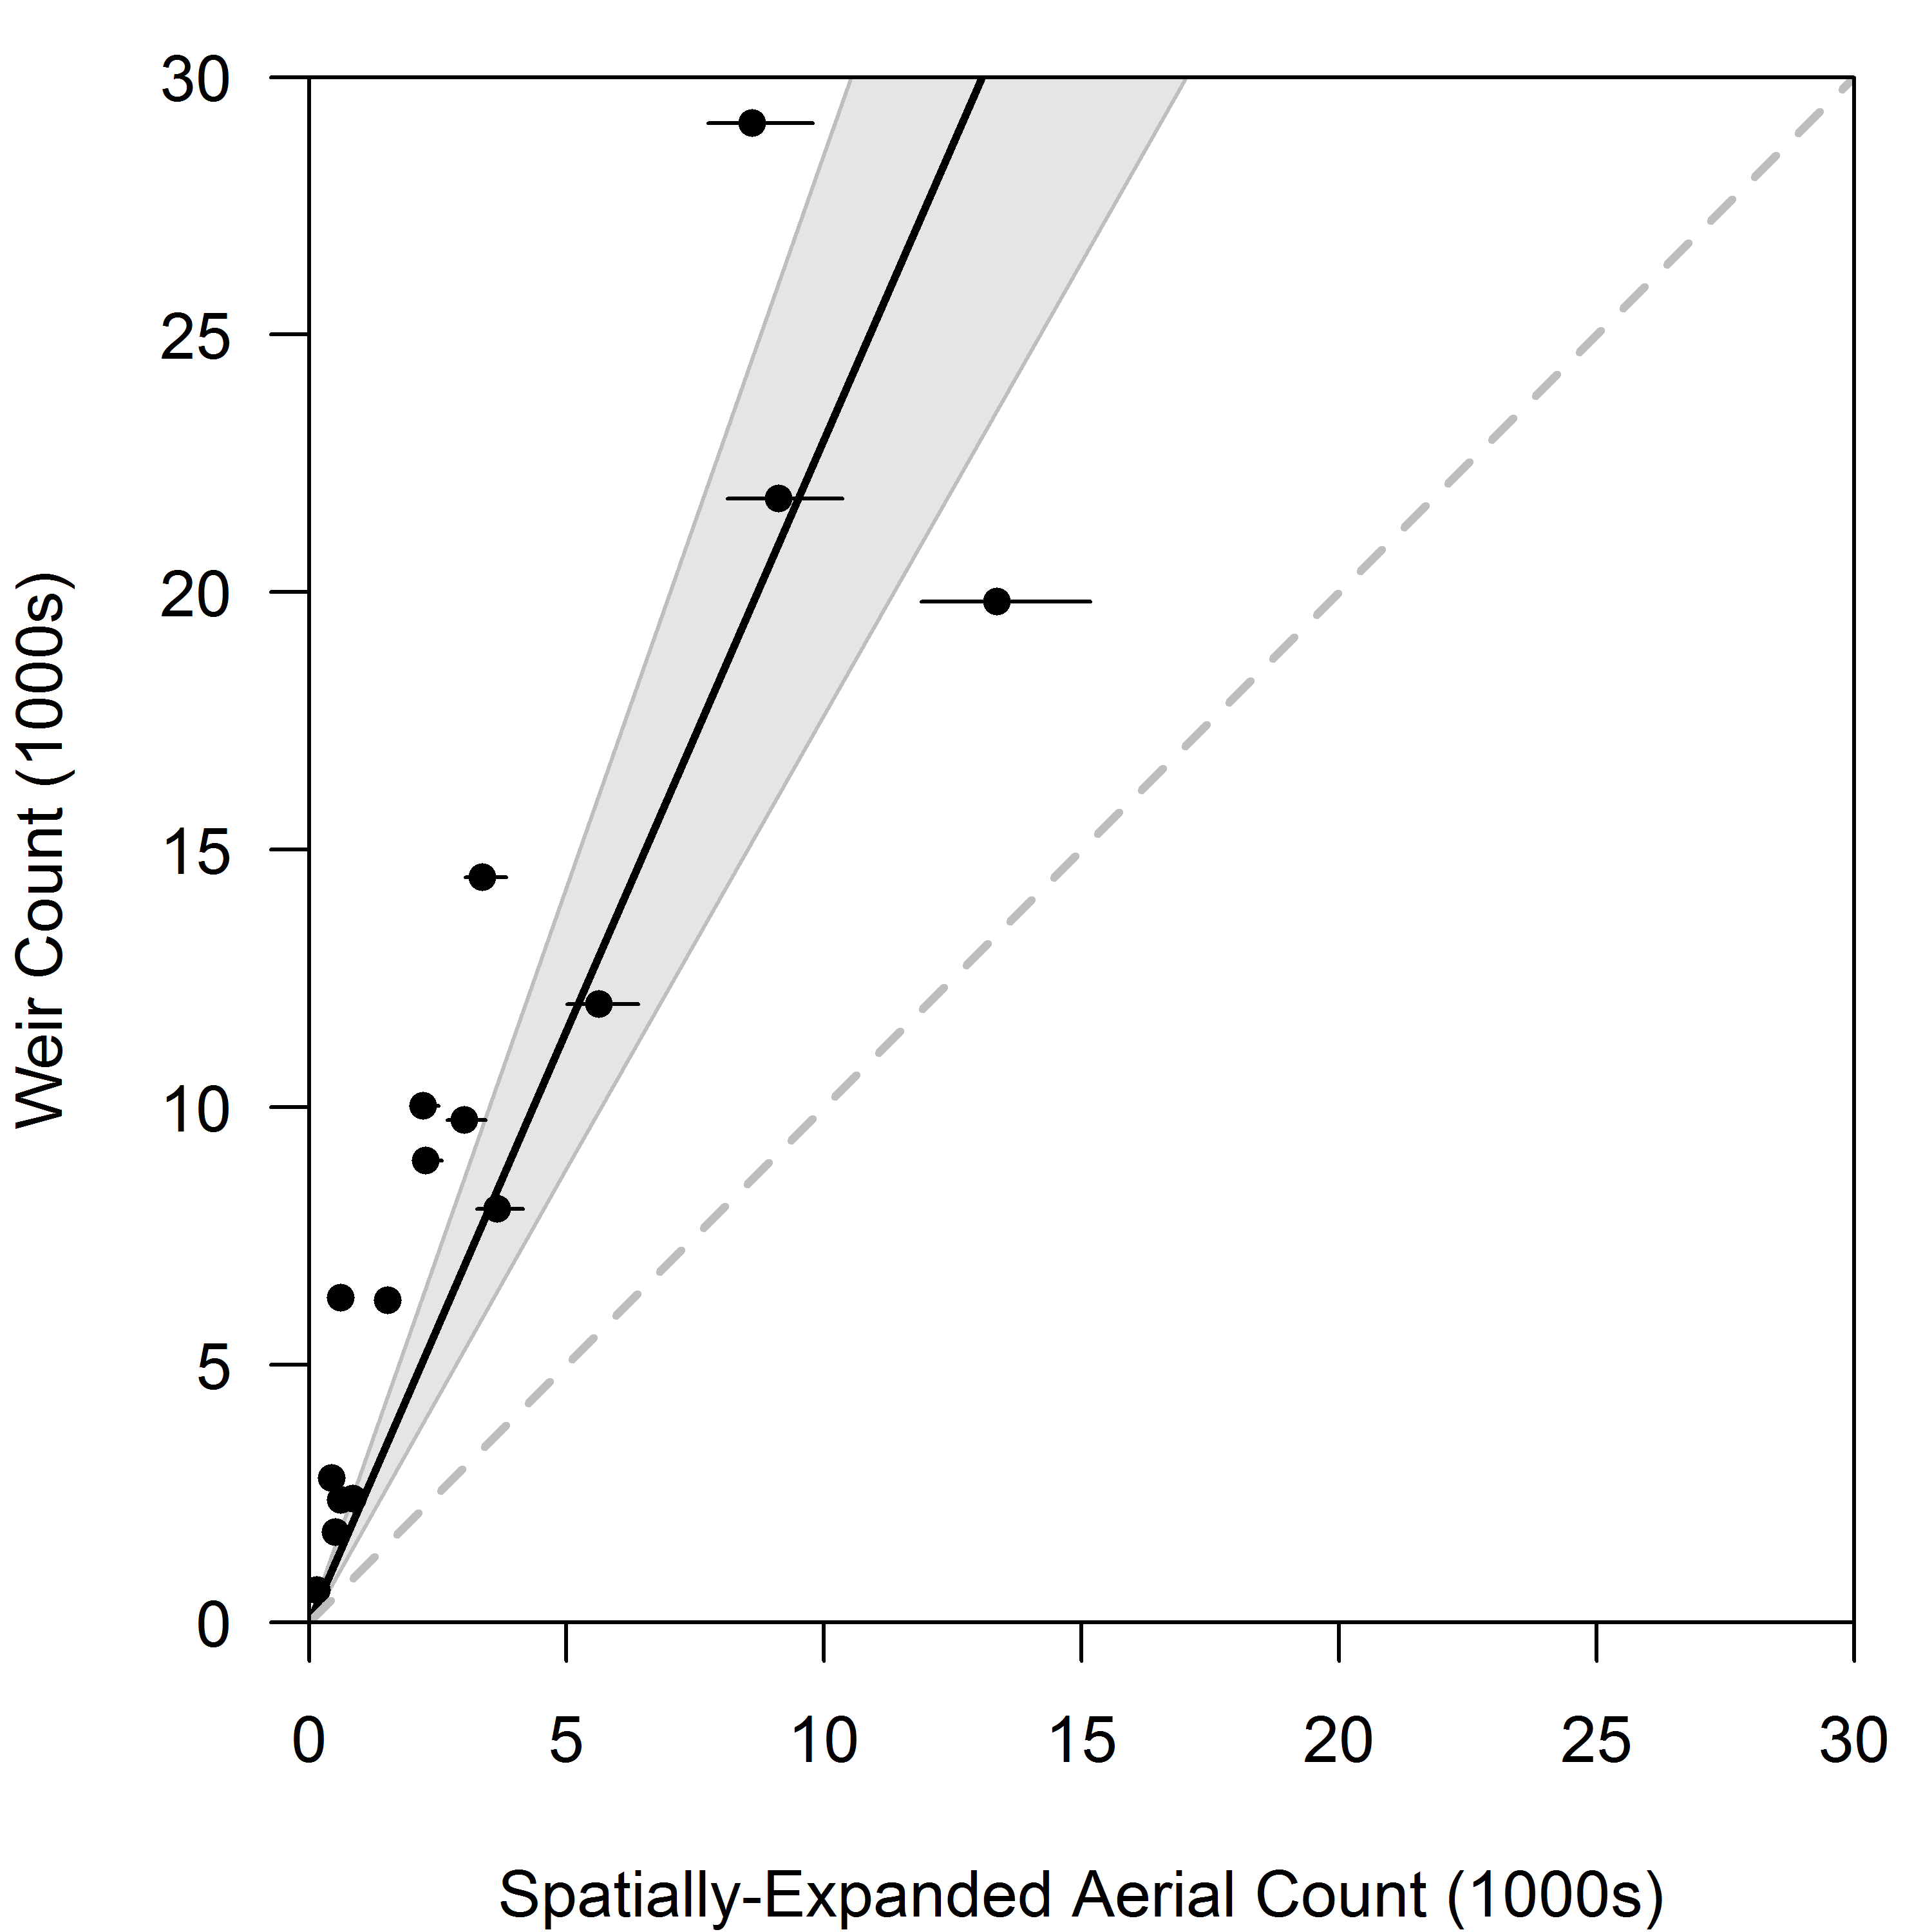
\includegraphics{img/Ch4/obs-correct.png}
  \caption{The relationship between spatially-expanded aerial survey estimates and weir counts during the same years and substocks as described by (\ref{eq:temp-expand1}). Notice the uncertainty expressed in the predictor variable; this was included in the analysis by incorporating both the spatial (Section \ref{spat-expansion}) and temporal (Section \ref{temp-expansion}) expansions in a single model fitted using Bayesian methods.}
  \label{fig:obs-correct}
\end{figure}

\clearpage

\begin{figure}
  \centering
  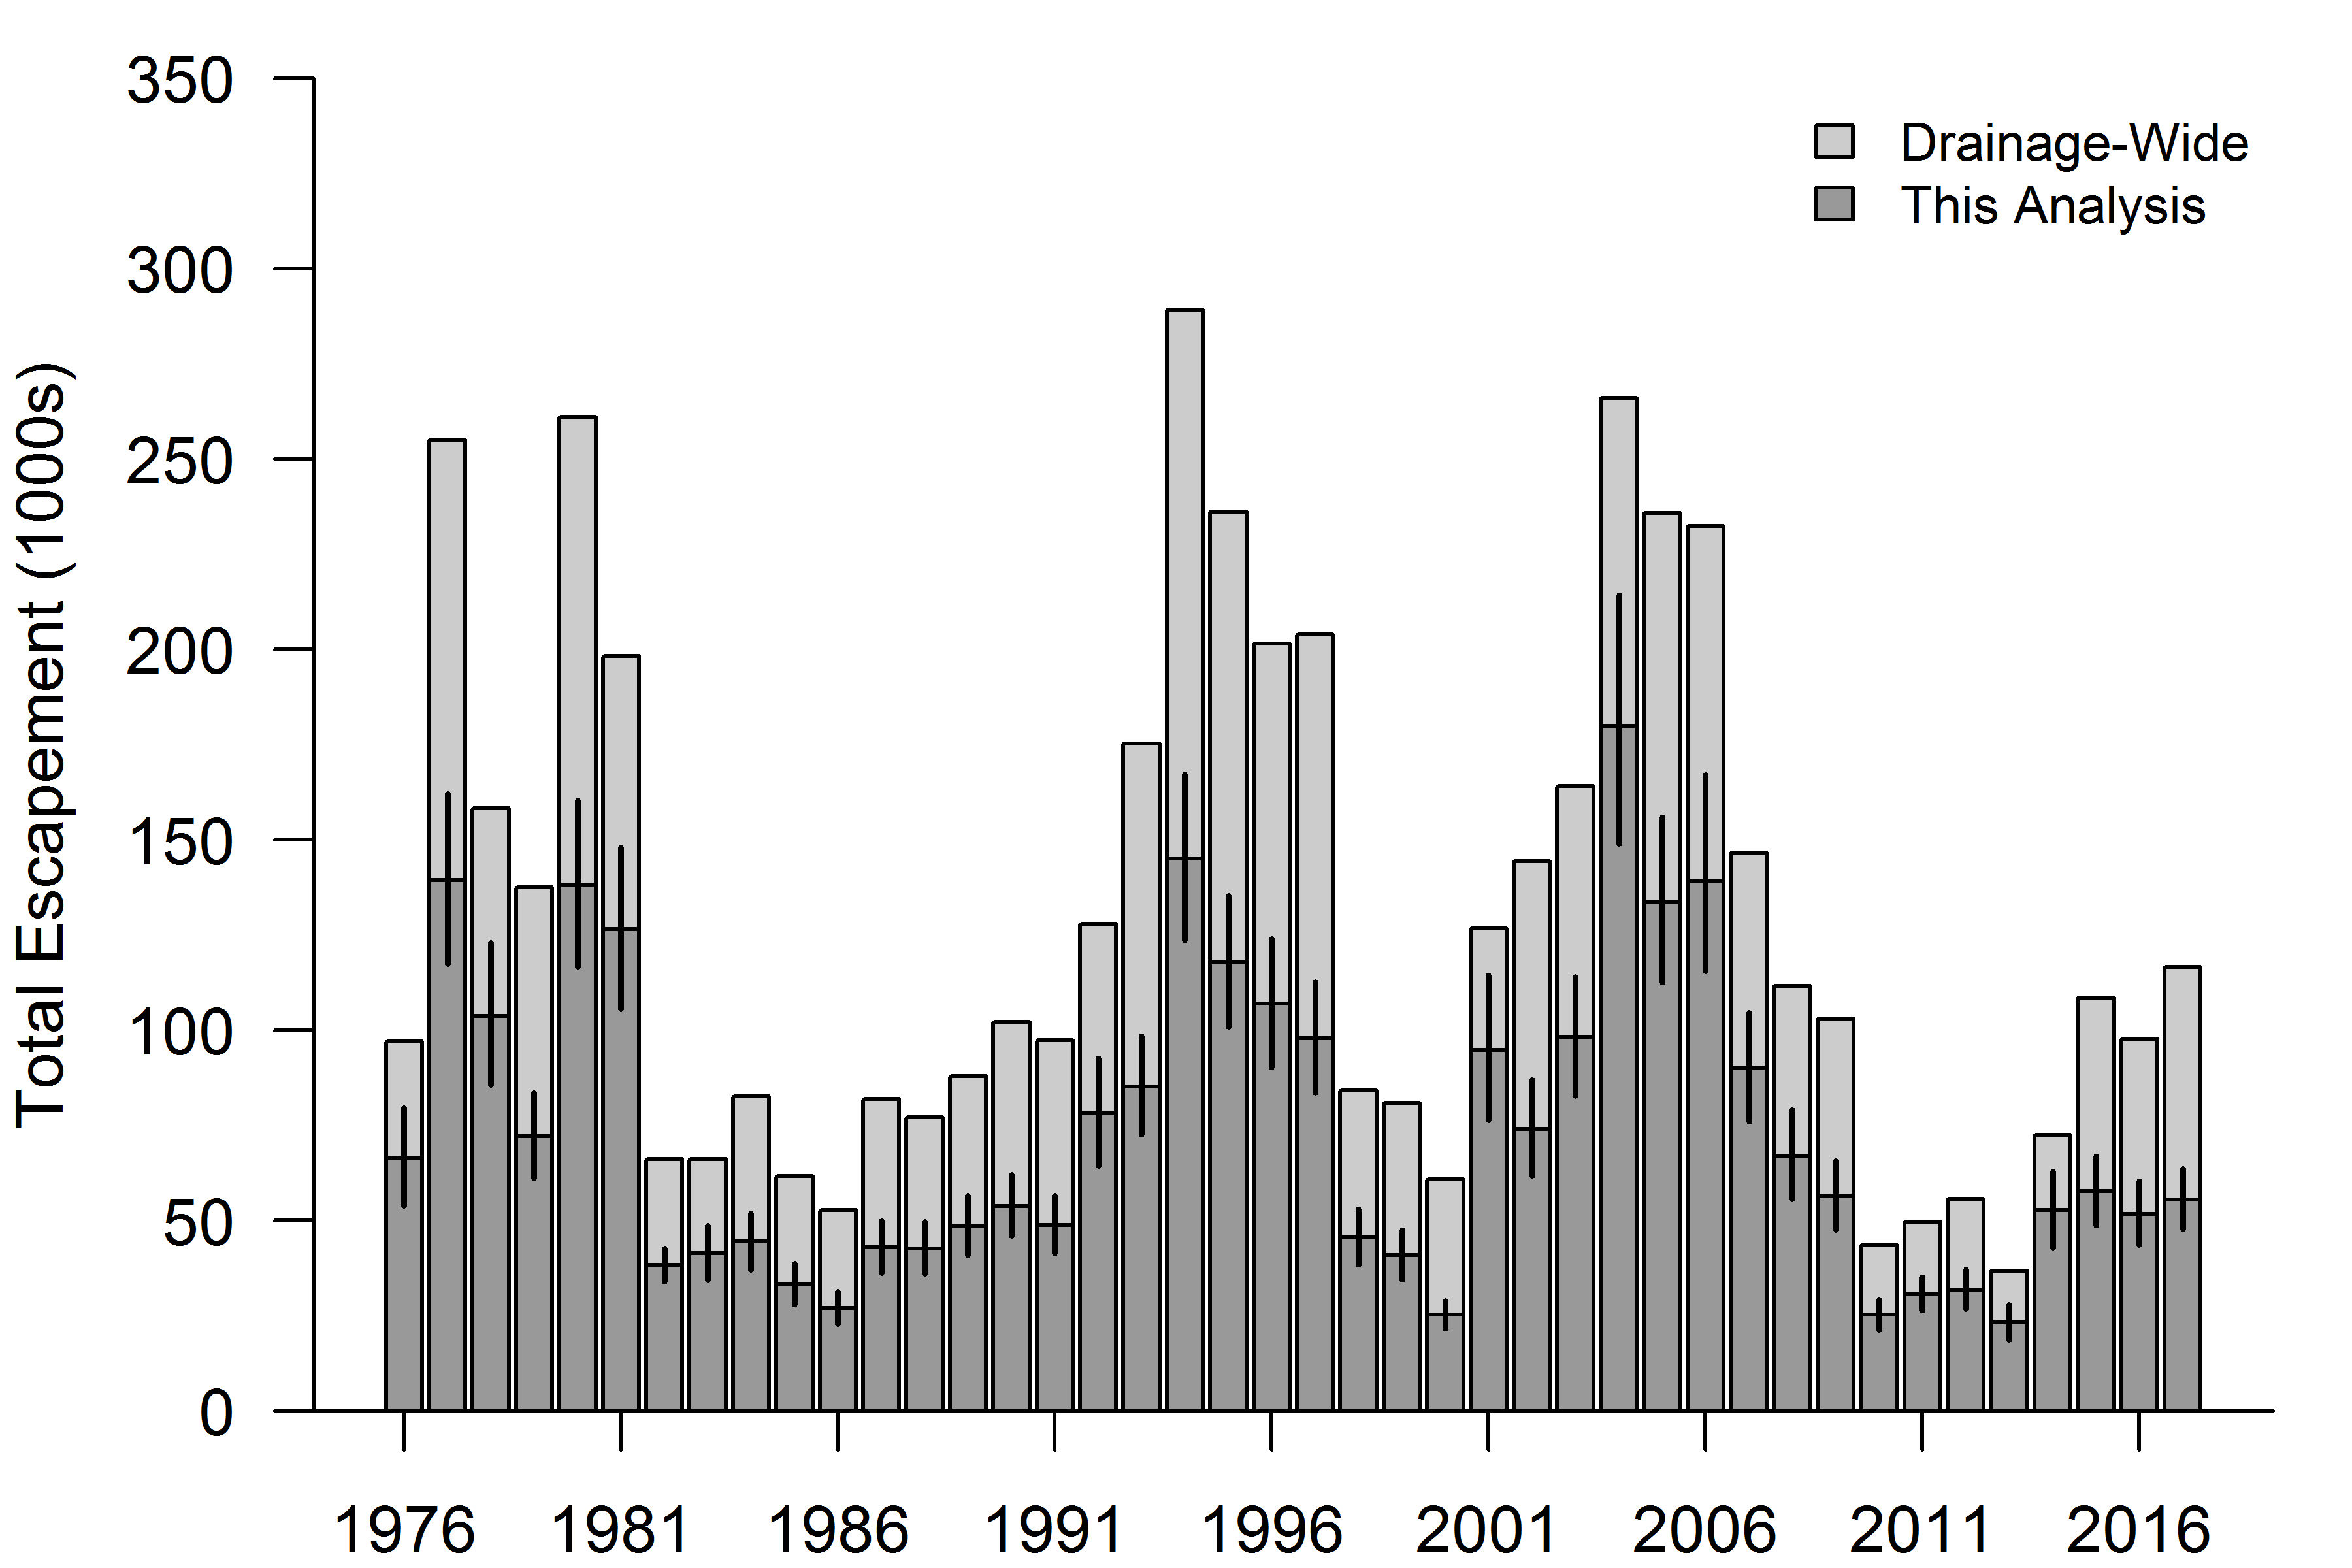
\includegraphics{img/Ch4/obs-fraction.png}
  \caption{Estimated Chinook salmon escapement for substocks within the Kuskokwim River drainage. `Drainage-wide' refers to the aggregate population estimates provided by a maximum likelihood run reconstruction model. `This analysis' refers to the estimated portion of the aggregate run included in this analysis (not all tributaries have been monitored).}
  \label{fig:obs-fraction}
\end{figure}

\bibliography{cites-without-doi.bib,cites-with-doi.bib}


\end{document}
